%% abtex2-modelo-trabalho-academico.tex, v-1.9.2 laurocesar
%% Copyright 2012-2014 by abnTeX2 group at http://abntex2.googlecode.com/ 
%%
%% This work may be distributed and/or modified under the
%% conditions of the LaTeX Project Public License, either version 1.3
%% of this license or (at your option) any later version.
%% The latest version of this license is in
%%   http://www.latex-project.org/lppl.txt
%% and version 1.3 or later is part of all distributions of LaTeX
%% version 2005/12/01 or later.
%%
%% This work has the LPPL maintenance status `maintained'.
%% 
%% The Current Maintainer of this work is the abnTeX2 team, led
%% by Lauro César Araujo. Further information are available on 
%% http://abntex2.googlecode.com/
%%
%% This work consists of the files abntex2-modelo-trabalho-academico.tex,
%% abntex2-modelo-include-comandos and abntex2-modelo-references.bib
%%

% ------------------------------------------------------------------------
% ------------------------------------------------------------------------
% abnTeX2: Modelo de Trabalho Academico (tese de doutorado, dissertacao de
% mestrado e trabalhos monograficos em geral) em conformidade com 
% ABNT NBR 14724:2011: Informacao e documentacao - Trabalhos academicos -
% Apresentacao
% ------------------------------------------------------------------------
% ------------------------------------------------------------------------

\documentclass[
	% -- opções da classe memoir --
	12pt,				% tamanho da fonte
	openright,			% capítulos começam em pág ímpar (insere página vazia caso preciso)
	twoside,			% para impressão em verso e anverso. Oposto a oneside
	a4paper,			% tamanho do papel. 
	% -- opções da classe abntex2 --
	%chapter=TITLE,		% títulos de capítulos convertidos em letras maiúsculas
	%section=TITLE,		% títulos de seções convertidos em letras maiúsculas
	%subsection=TITLE,	% títulos de subseções convertidos em letras maiúsculas
	%subsubsection=TITLE,% títulos de subsubseções convertidos em letras maiúsculas
	% -- opções do pacote babel --
	english,			% idioma adicional para hifenização
	french,				% idioma adicional para hifenização
	spanish,			% idioma adicional para hifenização
	brazil				% o último idioma é o principal do documento
	]{abntex2}

% ---
% Pacotes básicos 
% ---
\usepackage{lmodern}			% Usa a fonte Latin Modern			
\usepackage[T1]{fontenc}		% Selecao de codigos de fonte.
\usepackage[utf8]{inputenc}		% Codificacao do documento (conversão automática dos acentos)
\usepackage{lastpage}			% Usado pela Ficha catalográfica
\usepackage{indentfirst}		% Indenta o primeiro parágrafo de cada seção.
\usepackage{color}				% Controle das cores
\usepackage{graphicx}			% Inclusão de gráficos
\usepackage{microtype} 			% para melhorias de justificação
\usepackage{pdfpages}           % para inserir documentos em PDF
\usepackage{float}              % para determinar o local das imagens no texto
\usepackage{amssymb}            % pacote de matemática
\usepackage{verbatim}           % para comentar blocos
\usepackage{amsmath}            % pacote de matemática
\usepackage{verbatim}           % include .txt files
\usepackage[boxruled,linesnumbered,portuguese,portuguesekw]{algorithm2e} %insere algoritmos
\usepackage[section]{placeins}  %não deixa imagens ultrapassarem barreira
\usepackage{afterpage}          %insere figuras em uma página dedicada
% ---
		
% ---
% Pacotes adicionais, usados apenas no âmbito do Modelo Canônico do abnteX2
% ---
\usepackage{lipsum}				% para geração de dummy text
% ---

% ---
% Pacotes de citações
% ---
\usepackage[brazilian,hyperpageref]{backref}	 % Paginas com as citações na bibl
\usepackage[alf]{abntex2cite}	% Citações padrão ABNT

% --- 
% CONFIGURAÇÕES DE PACOTES
% --- 

% ---
% Configurações do pacote backref
% Usado sem a opção hyperpageref de backref
\renewcommand{\backrefpagesname}{Citado na(s) página(s):~}
% Texto padrão antes do número das páginas
\renewcommand{\backref}{}
% Define os textos da citação
\renewcommand*{\backrefalt}[4]{
	\ifcase #1 %
		Nenhuma citação no texto.%
	\or
		Citado na página #2.%
	\else
		Citado #1 vezes nas páginas #2.%
	\fi}%
% ---

% ---
% Informações de dados para CAPA e FOLHA DE ROSTO
% ---
\titulo{Modelagem geológica implícita com funções distância assinaladas}
\autor{Roberto Mentzingen Rolo}
\local{Porto Alegre}
\data{2017}
\orientador{Prof. Dr. João Felipe Coimbra Leite Costa}
%\coorientador{Equipe \abnTeX}
\instituicao{%
  Universidade Federal do Rio Grande do Sul - UFRGS
  \par
  Escola de Engenharia
  \par
  Programa de Pós-Graduação em Enhenharia de Minas, Metalúrgica e de Materiais}
\tipotrabalho{Dissertação (Mestrado)}
% O preambulo deve conter o tipo do trabalho, o objetivo, 
% o nome da instituição e a área de concentração 
\preambulo{Esta dissertação foi analisada e julgada adequada para a obtenção do título de Mestre em Engenharia, área de concentração de Tecnologia Mineral, e aprovada em sua forma final pelo Orientador e pela Banca Examinadora designada pelo Programa de Pós-Graduação em Engenharia de Minas, Metalúrgica e de Materiais da Universidade Federal do Rio Grande do Sul.}
% ---

% ---
% Configurações de aparência do PDF final

% alterando o aspecto da cor azul
\definecolor{blue}{RGB}{41,5,195}

% informações do PDF
\makeatletter
\hypersetup{
     	%pagebackref=true,
		pdftitle={\@title}, 
		pdfauthor={\@author},
    	pdfsubject={\imprimirpreambulo},
	    pdfcreator={LaTeX with abnTeX2},
		pdfkeywords={abnt}{latex}{abntex}{abntex2}{trabalho acadêmico}, 
		colorlinks=true,       		% false: boxed links; true: colored links
    	linkcolor=blue,          	% color of internal links
    	citecolor=blue,        		% color of links to bibliography
    	filecolor=magenta,      		% color of file links
		urlcolor=blue,
		bookmarksdepth=4
}
\makeatother
% --- 

% --- 
% Espaçamentos entre linhas e parágrafos 
% --- 

% O tamanho do parágrafo é dado por:
\setlength{\parindent}{1.3cm}

% Controle do espaçamento entre um parágrafo e outro:
\setlength{\parskip}{0.2cm}  % tente também \onelineskip

% ---
% compila o indice
% ---
\makeindex
% ---

% ----
% Início do documento
% ----
\begin{document}

% Retira espaço extra obsoleto entre as frases.
\frenchspacing 

% ----------------------------------------------------------
% ELEMENTOS PRÉ-TEXTUAIS
% ----------------------------------------------------------
% \pretextual

% ---
% Capa
% ---
\imprimircapa
% ---

% ---
% Folha de rosto
% (o * indica que haverá a ficha bibliográfica)
% ---
\imprimirfolhaderosto*
% ---

% ---
% Inserir a ficha bibliografica
% ---

% Isto é um exemplo de Ficha Catalográfica, ou ``Dados internacionais de
% catalogação-na-publicação''. Você pode utilizar este modelo como referência. 
% Porém, provavelmente a biblioteca da sua universidade lhe fornecerá um PDF
% com a ficha catalográfica definitiva após a defesa do trabalho. Quando estiver
% com o documento, salve-o como PDF no diretório do seu projeto e substitua todo
% o conteúdo de implementação deste arquivo pelo comando abaixo:
%
% \begin{fichacatalografica}
%     \includepdf{fig_ficha_catalografica.pdf}
% \end{fichacatalografica}
\begin{fichacatalografica}
	\vspace*{\fill}					% Posição vertical
	\hrule							% Linha horizontal
	\begin{center}					% Minipage Centralizado
	\begin{minipage}[c]{12.5cm}		% Largura
	
	\imprimirautor
	
	\hspace{0.5cm} \imprimirtitulo  / \imprimirautor. --
	\imprimirlocal, \imprimirdata-
	
	\hspace{0.5cm} \pageref{LastPage} p. : il. (algumas color.) ; 30 cm.\\
	
	\hspace{0.5cm} \imprimirorientadorRotulo~\imprimirorientador\\
	
	\hspace{0.5cm}
	\parbox[t]{\textwidth}{\imprimirtipotrabalho~--~\imprimirinstituicao,
	\imprimirdata.}\\
	
	\hspace{0.5cm}
		1. modelagem geológica.
		2. modelagem geológica implícita.
        3. funções distância assinaladas
		I. Prof. Dr. João Felipe Coimbra Leite Costa.
		II. Universidade Federal do Rio Grande do Sul.
		III. Faculdade de Engenharia.
		IV. Modelagem geológica implícita com funções distância assinaladas\\ 			
	
	\hspace{8.75cm} CDU 02:141:005.7\\
	
	\end{minipage}
	\end{center}
	\hrule
\end{fichacatalografica}
% ---

% ---
% Inserir errata
% ---
%\begin{errata}
%Elemento opcional da \citeonline[4.2.1.2]{NBR14724:2011}. Exemplo:
%
%\vspace{\onelineskip}
%
%FERRIGNO, C. R. A. \textbf{Tratamento de neoplasias ósseas apendiculares com
%reimplantação de enxerto ósseo autólogo autoclavado associado ao plasma
%rico em plaquetas}: estudo crítico na cirurgia de preservação de membro em
%cães. 2011. 128 f. Tese (Livre-Docência) - Faculdade de Medicina Veterinária e
%Zootecnia, Universidade de São Paulo, São Paulo, 2011.
%
%\begin{table}[htb]
%\center
%\footnotesize
%\begin{tabular}{|p{1.4cm}|p{1cm}|p{3cm}|p{3cm}|}
%  \hline
%   \textbf{Folha} & \textbf{Linha}  & \textbf{Onde se lê}  & \textbf{Leia-se}  \\
%    \hline
%    1 & 10 & auto-conclavo & autoconclavo\\
%   \hline
%\end{tabular}
%\end{table}
%
%\end{errata}
% ---

% ---
% Inserir folha de aprovação
% ---

% Isto é um exemplo de Folha de aprovação, elemento obrigatório da NBR
% 14724/2011 (seção 4.2.1.3). Você pode utilizar este modelo até a aprovação
% do trabalho. Após isso, substitua todo o conteúdo deste arquivo por uma
% imagem da página assinada pela banca com o comando abaixo:
%
% \includepdf{folhadeaprovacao_final.pdf}
%
\begin{folhadeaprovacao}

  \begin{center}
    {\ABNTEXchapterfont\large\imprimirautor}

    \vspace*{\fill}\vspace*{\fill}
    \begin{center}
      \ABNTEXchapterfont\bfseries\Large\imprimirtitulo
    \end{center}
    \vspace*{\fill}
    
    \hspace{.45\textwidth}
    \begin{minipage}{.5\textwidth}
        \imprimirpreambulo
    \end{minipage}%
    \vspace*{\fill}
   \end{center}
        
   Trabalho aprovado. \imprimirlocal, 24 de fevereiro de 2017:

   \assinatura{\textbf{Prof. Dr. André Cezar Zingano} \\ PPGE3M - UFRGS} 
   \assinatura{\textbf{Prof. Dr. Diego Machado Marques} \\ Convidado externo ao PPGE3M}
   \assinatura{\textbf{Dr. Marcelo Cheviche Godoy} \\ Newmont Mining Corporation}
   %\assinatura{\textbf{Professor} \\ Convidado 3}
   %\assinatura{\textbf{Professor} \\ Convidado 4}
      
   \begin{center}
    \vspace*{0.5cm}
    {\large\imprimirlocal}
    \par
    {\large\imprimirdata}
    \vspace*{1cm}
  \end{center}
  
\end{folhadeaprovacao}
% ---

% ---
% Dedicatória
% ---
%\begin{dedicatoria}
%   \vspace*{\fill}
%   \centering
%   \noindent
%   \textit{ Este trabalho é dedicado às crianças adultas que,\\
%   quando pequenas, sonharam em se tornar cientistas.} \vspace*{\fill}
%\end{dedicatoria}
% ---

% ---
% Agradecimentos
% ---
\begin{agradecimentos}

Ao Professor João Felipe por compartilhar um pouco do imenso conhecimento e pela recepção de braços abertos no laboratório. Aos colegas do LPM que contribuíram para o desenvolvimento desse trabalho, Ricardo Radkte, David Drummond, Áttila Leães e Péricles Machado. Aos demais colegas de laboratório, em especial, Ryu Okada, Marcel Bassani, Cristina Araújo, Augusto Torres, Anuar Bergamaschi, Lucas Roncarati, Marcelo Batelocchi, Ricardo Hundelshaussen, Ricardo Rodrigues, José Guilherme e George Gasper. Aos ICs, Rafael e Bento.

À minha família, em especial, Custódia e Marcelo pelo suporte. À Camila pelo companheirismo e incondicional apoio.

Ao Conselho Nacional de Desenvolvimento Científico e Tecnológico (CNPq) pela bolsa concedida. À Newmont pelo apoio e informação fornecida à essa dissertação.

\end{agradecimentos}
% ---

% ---
% Epígrafe
% ---
\begin{epigrafe}
    \vspace*{\fill}
	\begin{flushright}
		\textit{``Life is made of choices \\
		Full of opportunities \\
		All we have to do is \\
		Recognize the pieces of the game\\
        Make out what is substancial\\
        And be proud of our undying past''\\
		(Reffer - Hidden Scars)}
	\end{flushright}
\end{epigrafe}
% ---

% ---
% RESUMOS
% ---

% resumo em português
\setlength{\absparsep}{18pt} % ajusta o espaçamento dos parágrafos do resumo
\begin{resumo}
Previamente à cada estimativa ou simulação geoestatística os domínios geológicos do depósito devem ser modelados, o que tradicionalmente é feito de forma manual por um geomodelador, em um processo laborioso, demorado e subjetivo. Por essa razão novas técnicas conhecidas como métodos implícitos veem surgindo. Essas técnicas fornecem algoritmos que substituem o processo de digitalização manual dos métodos explícitos por alguma forma de procedimento automático. Essa dissertação visita alguns métodos implícitos bem estabelecidos com atenção especial à modelagem geológica implícita com funções distância assinalada. Um estudo de caso em um banco de dados real é apresentado e a aplicabilidade do método discutida. Embora não substitua por completo um geomodelador experiente, o método provou ser capaz de gerar modelos geológicos semi-automáticos realistas a partir dos dados amostrais, e se mostra útil principalmente nas fases iniciais da pesquisa mineral.  

 \textbf{Palavras-chaves}: modelagem geológica, modelagem geológica implícita, funções distância assinaladas.
\end{resumo}

% resumo em inglês
\begin{resumo}[Abstract]
 \begin{otherlanguage*}{english}
Prior to every geostatistical estimation or simulation study there is a need for delimiting the geologic domains of the deposit, which is traditionally done manually by a geomodeler in a laborious, time consuming and subjective process. For this reason, novel techniques referred to as implicit modelling have appeared. These techniques provide algorithms that replace the manual digitization process of the traditional methods by some form of automatic procedure. This dissertation covers a few well established implicit methods currently available with special attention to the signed distance function methodology. A case study based on a real dataset was performed and its applicability discussed. Although it did not replace an experienced geomodeler, the method proved to be capable in creating semi-automatic geological models from the sampling data, especially in the early stages of exploration.

   \vspace{\onelineskip}
 
   \noindent 
   \textbf{Key-words}: geologic modeling, implicit geologic modeling, signed distance function, domaining.
 \end{otherlanguage*}
\end{resumo}

% resumo em francês 
%\begin{resumo}[Résumé]
% \begin{otherlanguage*}{french}
%    Il s'agit d'un résumé en français.
% 
%   \textbf{Mots-clés}: latex. abntex. publication de textes.
% \end{otherlanguage*}
%\end{resumo}

% resumo em espanhol
%\begin{resumo}[Resumen]
% \begin{otherlanguage*}{spanish}
%   Este es el resumen en español.
%  
%   \textbf{Palabras clave}: latex. abntex. publicación de textos.
% \end{otherlanguage*}
%\end{resumo}
% ---

% ---
% inserir lista de ilustrações
% ---
\pdfbookmark[0]{\listfigurename}{lof}
\listoffigures*
\cleardoublepage
% ---

% ---
% inserir lista de tabelas
% ---
\pdfbookmark[0]{\listtablename}{lot}
\listoftables*
\cleardoublepage
% ---

% ---
% inserir lista de abreviaturas e siglas
% ---
%\begin{siglas}
%\end{siglas}
% ---

% ---
% inserir lista de símbolos
% ---
%\begin{simbolos}
%\end{simbolos}
% ---

% ---
% inserir o sumario
% ---
\pdfbookmark[0]{\contentsname}{toc}
\tableofcontents*
\cleardoublepage
% ---



% ----------------------------------------------------------
% ELEMENTOS TEXTUAIS
% ----------------------------------------------------------
\textual

\chapter{Introdução}

\citeonline{hustrulid2013open} fragmentam a evolução de uma mina em três fases distintas: (1) Planejamento, (2) Implementação e (3) Produção. A \autoref{seq_min} é uma linha do tempo mostrando a relação entre as diferentes fases e seus estágios. Na fase de planejamento os depósitos minerais são investigados no que diz respeito à sua atratividade econômica e exequibilidade técnica. A fase de planejamento culmina em um relatório de viabilidade, no qual é baseada a decisão de investir e dar continuidade ao empreendimento mineiro, iniciando a fase de implementação, período de maior fluxo de caixa, quando mina e usina de processamento são desenvolvidas. Finalmente a mina entra em operação, o minério é explotado e processado, e o produto vendido no mercado.     

\begin{figure}[!htb]
	\caption{\label{seq_min}Fases da mineração.}
	\begin{center}
		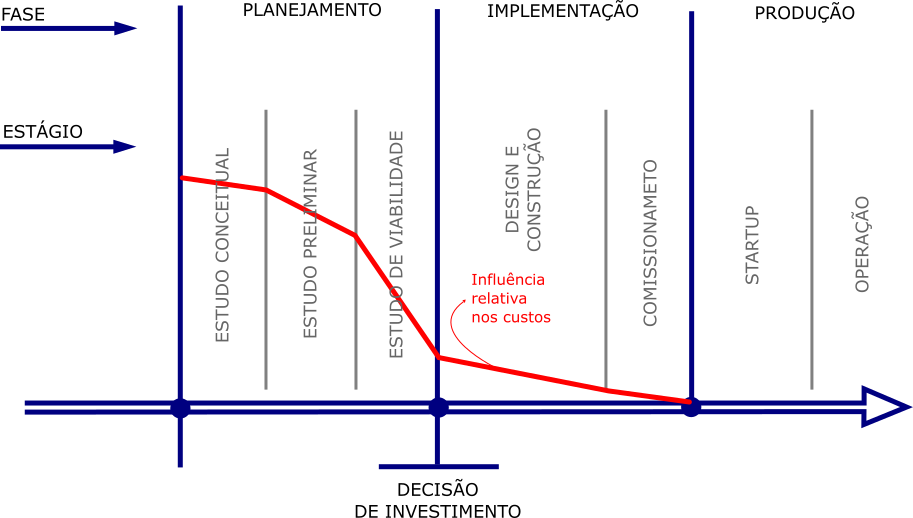
\includegraphics[width=0.6\textwidth]{introducao/min_fases}
	\end{center}
	\legend{Modificado de \citeonline{hustrulid2013open}}
\end{figure}

A avaliação das reservas é parte fundamental e alicerce do estudo de viabilidade, os teores e tonelagens são quantificados e modelos numéricos que caracterizam a geologia em subsuperfície criados com base nos dados de sondagem. A partir desses modelos, engenheiros e geólogos planejam e tomam as decisões econômicas e técnicas: Escolha do método de lavra, alternativas de processamento mineral, operações auxiliares, estimativas de custos operacionais, capital de investimento e projeção do lucro. Como resultado, uma estratégia que determina quanto material será removido ano a ano é traçada. O projeto determina os limites econômicos da mina e a sequência ótima de lavra bloco a bloco, baseado no modelo geoestatístico de blocos.

Na fase de planejamento é possível  minimizar o capital e custo operacional do projeto final e ao mesmo tempo maximizar a operabilidade e lucro. A influência relativa nos custos de cada fase é mostrado na linha vermelha da \autoref{seq_min} \cite{hustrulid2013open}. A principal causa de fracasso em empreendimentos mineiros é falta de conhecimento a respeito do corpo mineralizado. Isto posto, estimativas precisas e acuradas são importantes. Até mesmo um pequeno desvio entre produção planejada e real pode causar sérios prejuízos financeiros.
 
A avaliação dos recursos de uma mina é composta de duas etapas \cite{chiles2004modelling}: (1) delimitação das várias unidades geológicas, correspondentes às diferentes formações geológicas ou diferentes litologias; (2) estimativas e/ou simulação de teores em cada unidade modelada.

Desse modo, previamente à toda estimativa e/ou simulação de teores, há a necessidade de delimitar as unidades geológicas, implicando em decisão de estacionariedade e homogeneidade mineralógica em cada domínio modelado. Isto é, Os teores de cada domínio geológico pertencem a diferentes populações estatísticas e são caracterizados através de modelos de distribuição e semivariogramas específicos, resultando em estimativas e/ou simulações distintas para cada população \cite{mclennan}.

Modelos geológicos descrevem a extensão, forma e volume das diferentes unidades geológicas no espaço. Gerar modelos geológicos corretos é necessário para que estimativas mais precisas de volume/massa e teores sejam obtidas e problemas de diluição ocasionados pela falta de aderência do modelo de blocos às estruturas geológicas do depósito sejam reduzidos \cite{rasera2014estrati}.

Tradicionalmente os modelos geológicos são criados explicitamente, através de um processo de digitalização dos contatos geológicos. Polígonos são construídos manualmente em seções, por um geomodelador, honrando os dados amostrais, esses polígonos são conectados por linhas-guia e então interpolados por triangulação, gerando sólidos que representam as unidades geológicas. Esse processo apresenta alguns pontos críticos segundo \citeonline{cowan2003practical}:
\begin{itemize}
\item É demorado e requer um geomodelador experiente; 
\item É subjetivo, já que cada geomodelador interpretará, e produzirá um modelo diferente a partir do mesmo banco de dados, tornando replicação e auditoria externa do modelo tarefas árduas;
\item  É inflexível, pois atualizar o modelo à medida que novos dados são adquiridos é demorado e laborioso. 
\end{itemize}

Para muitas minas, apenas um único modelo geológico é mantido, dada a limitação de tempo imposta pelos métodos explícitos. Raramente há oportunidade de modelar interpretações alternativas e comparar estimativas de recursos baseadas em diferentes modelos. Não havendo assim, oportunidade de avaliar as incertezas inerentes ao modelamento geológico \cite{cowan2003practical}.

Ainda que \textit{softwares} modernos de mineração forneçam ferramentas computacionais para visualizar os dados de sondagem e agilizar o processo de digitalização manual, os métodos explícitos ainda sofrem com as desvantagens apresentadas. Por esse motivo, novas técnicas, conhecidas como modelagem implícita, vêm surgindo. São algoritmos que reduzem o nível de subjetividade, substituindo o processo de digitalização manual por alguma forma de procedimento automático \cite{maureira}.

As técnicas de modelagem geológica implícita se dividem em dois grandes grupos: 

O grupo das técnicas determinísticas. Métodos diretos e computacionalmente rápidos. Alguns métodos estabelecidos nessa categoria são a interpolação suavizada discreta \cite{mallet2002geomodeling}, o método dos campos potenciais \cite{chiles2004modelling,calcagno2008geological,renard2013modeling}, operacionalizado no \textit{software Isatis}\textsuperscript{\textregistered}, e a metodologia implementada no \textit{software} de modelagem geológica \textit{Leapfrog}\textsuperscript{\textregistered} \cite{cowan2002rapid,cowan2003practical}, amplamente utilizado pela indústria.

O outro grupo compreende as técnicas estocásticas de modelagem geológica. Métodos complexos que demandam grande esforço computacional. Entretanto, no lugar de um único modelo geológico, esses métodos geram diversas realizações equiprováveis da distribuição espacial das diferentes litologias, reproduzindo os atributos estatísticos das amostras. Assim, a partir da análise conjunta das realizações é possível avaliar a incerteza associada ao modelo geológico. 

São métodos consolidados: A simulação sequencial dos indicadores \cite{journel1983nonparametric}, simulação sequencial gaussiana truncada \cite{journel1984conditional}, simulação plurigaussiana \cite{galli1994pros}, métodos baseados em simulação objetos (\textit{object-based}) \cite{bridge1979simulation}, recentemente surgiram os métodos de modelagem de superfície (\textit{surface-based}) \cite{pyrcz2005stochastic}. Contudo, os algoritmos tradicionais de simulação, baseados em estatísticas de dois pontos, não são capazes de reproduzir estruturas geológicas que apresentam complexas interdependências, assim surgem os métodos baseados em geoestatística multiponto (MPS) \cite{guardiano1993multivariate}.

\citeonline{silvaanddeutschccgmodeling} apresentaram a modelagem geológica implícita com funções distância assinaladas para modelar múltiplos domínios geológicos simultaneamente. \citeonline{deutschcoal} o utilizou para modelar múltiplas camadas de carvão, e mostrou que o método é uma poderosa ferramenta de modelagem. \citeonline{wildedeutschcalibrate} e \citeonline{silvaanddeutschccgcorrecting} introduziram duas medidas heurísticas diferentes de avaliação de incertezas e \citeonline{silvaanddeutschccgcorrecting} uma ferramenta para corrigir as proporções globais dos diferentes domínios. E mostraram, novamente, a competência do método. \citeonline{maureira} revisitou o método com a finalidade de construir, a partir dos dados amostrais, imagens de treinamento (\textit{data-driven training images}) que forneçam as estatísticas de múltiplos pontos (MPS) para a simulação de litologias. 

A modelagem geológica implícita com funções distância assinaladas é uma técnica determinística, baseada na interpolação de uma função distância em um \textit{grid}. Funções de distância assinaladas medem o grau de separação entre as diferentes litologias, e dependem da orientação, forma e extensão dos corpos geológicos. Distâncias positivas indicam o exterior do domínio enquanto distâncias negativas indicam o interior do domínio. As distâncias assinaladas são calculadas para cada ponto amostral e para cada litologia, e interpoladas para os locais não amostrados. Um modelo geológico é criado a partir dos valores estimados para as distâncias assinaladas. O método é computacionalmente eficiente, direto e não depende de funções matemáticas complicadas. Ainda assim, consegue reproduzir de maneira satisfatória estruturas geológicas de grande escala nos modelos numéricos \cite{maureira}.

Essa dissertação é uma extensão do trabalho de \citeonline{deutschcoal} e \citeonline{maureira}. Um \textit{plug-in} implementando o método no \textit{software SGeMS} foi desenvolvido e apresentado. A aplicabilidade do método mais uma vez foi posta à prova em um estudo de caso conduzido em um banco de dados real. E suas principais características, vantagens e limitações discutidas.

\section{Meta}

Essa dissertação de mestrado tem como meta investigar a aplicabilidade da modelagem geológica implícita com funções distância assinaladas como substituto ou método auxiliar à metodologia explícita de modelagem geológica, amplamente adotada pela indústria. Conhecidas as limitações e desvantagens da última e simplicidade e rapidez da primeira.

\section{Objetivos específicos}

A fim de atingir a meta proposta os seguintes objetivos foram delineados:
\begin{enumerate}
\item Operacionalizar o método no \textit{software} geoestatístico de código aberto \textit{SGeMS}, desenvolvendo um \textit{plug-in} funcional em \textit{python};
\item Conduzir um estudo de caso em um banco de dados real e verificar a qualidade do modelo gerado pela metodologia proposta, comparando-o a um modelo de referência.
\end{enumerate}

\section{Metodologia}

A partir de um banco de dados categóricos o valor da função distância assinalada é calculado para cada litologia em cada ponto amostral. As distâncias calculadas são então variografadas e interpoladas, por krigagem ordinária, para todo o \textit{grid}. Assim, o valor da função distância assinalada é conhecido em todos os nós e para cada litologia. Um modelo geológico pode ser criado diretamente a partir do valor estimado para as distâncias. Ou então, modelos de probabilidade podem ser criados a partir das distâncias. E então, um modelo geológico, que tem as proporções corrigidas para corresponder a uma proporção alvo, criado a partir dos modelos de probabilidade. A \autoref{chart} ilustra o fluxograma do processo. 

\begin{figure}[!htb]
	\caption{\label{chart}Fluxograma ilustrando a metodologia passo a passo.}
	\begin{center}
		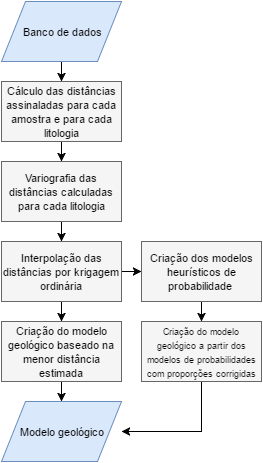
\includegraphics[width=0.4\textwidth]{introducao/chart1}
	\end{center}
	%\legend{Fonte: Modificado de \citeonline{hustrulid2013open}}
\end{figure}

O modelo criado implicitamente com a metodologia proposta foi comparado com um modelo criado explicitamente, a partir do mesmo banco de dados. Assim, foi possível checar se o algoritmo reproduziu satisfatoriamente as estruturas geológicas interpretadas pelo geomodelador.

\section{Estrutura da dissertação}

O capítulo 2 Revisa os conceitos de funções implícitas, estacionariedade e os principais métodos determinísticos de modelagem implícita baseados em funções implícitas: método dos campos potenciais, implementado no \textit{software Isatis}\textsuperscript{\textregistered}, e o método implementado no  \textit{software Leapfrog}\textsuperscript{\textregistered}.

O capítulo 3 apresenta o arcabouço teórico da modelagem geológica implícita com funções distância assinaladas, o \textit{plug-in} desenvolvido para o  \textit{software SGeMS} e os resultados da validação do algoritmo proposto tendo como referência resultados análogos da rotina \textit{DFMod} da biblioteca de algoritmos geoestatísticos \textit{GSLib}.

O capítulo 4 discute os resultados do estudo de caso conduzido em um banco de dados real, proveniente de um depósito de ouro. Avalia a aplicabilidade do método como substituto ou método auxiliar à metodologia tradicional (explicita) de modelagem geológica, comparando o modelo gerado a partir da metodologia proposta a um modelo de referência, criado explicitamente por um geomodelador. 

O capítulo 5 encerra a dissertação apresentando as conclusões do trabalho  e sugere trabalhos futuros relacionados ao tópico. 


\chapter{Revisão bibliográfica}

\section{Estacionariedade}
		
Nesta seção são apresentadas as definições de funções aleatórias e estacionariedade. Fundamentais ao pleno entendimento da necessidade da modelagem dos domínios geológicos de um depósito mineral sob o ponto de vista matemático. \cite{matheron1965variables, journel1978mining, armstrong1998basic}.
	
\subsection{Funções aleatórias}\label{func_al}
			
Um fenômeno natural pode muitas vezes ser caracterizado pela distribuição espacial de uma ou mais variáveis, chamadas variáveis regionalizadas (ReV).
			
Uma variável aleatória (RV), é uma variável que recebe um certo número de valores numéricos de acordo com uma determinada distribuição de probabilidade. O resultado do lançamento de um dado, por exemplo, pode ser considerado uma RV que pode receber um entre seis valores equiprováveis. 
			
Um valor observado em um ponto amostral $x_i$ é  a realização, $z(x_i)$ de uma variável regionalizada, $Z(x_i)$. A família de todas as variáveis aleatórias auto-correlacionadas $Z(x)$ quando $x$ varia por todo o domínio ($D$) de um depósito é uma função aleatória (RF) $\{Z(x),x\in D\}$. Essa definição de função aleatória expressa o aspecto aleatório e estruturado das variáveis regionalizadas.

Localmente, no ponto $x_i$, $Z(x_i)$ é uma variável aleatória. $Z(x)$ é uma RF, já que para cada par de pontos $x_i$ e $x_i+h$, as RV correspondentes, $Z(x_i)$ e $Z(x_i+h)$ não são independentes, são relacionadas por uma correlação que expressa a estrutura espacial da variável regionalizada $z(x)$.
			 
De acordo com \citeonline{journel1978mining}, o problema então, passa a ser representar a variabilidade da função aleatória no espaço (quando $x$ varia), essa representação será usada para resolver problemas de estimativa do valor $z(x_0)$ em um ponto $x_0$ que não foi amostrado.
			
A interpretação probabilística da Variável regionalizada $z(x)$ como sendo uma determinada realização de uma certa RF $Z(x)$ faz sentido apenas quando é possível inferir, mesmo que parcialmente, a lei de probabilidade que define a RF.
			
É virtualmente impossível inferir a lei de probabilidade de uma RF $Z(x)$ a partir de uma única realização $z(x)$, que por sua vez é limitada a um número finito de pontos amostrais $x_i$. Da mesma forma, é impossível determinar a lei de probabilidade que rege o lançamento de um dado a partir do resultado de um único lançamento, vários lançamentos são necessários para sua determinação. Várias realizações $z_1(x),z_2(x),...,z_k(x)$ da RF $Z(x)$ seriam necessárias para inferir a lei de probabilidade de $Z(x)$, na prática estamos limitados a uma única realização $\{z(x_i)\}$ da RF nas posições $x_i$, então, certas suposições envolvendo graus de homogeneidade espacial devem ser estabelecidas, a hipótese de estacionariedade.
			
Na prática, mesmo que apenas certa região do fenômeno possa ser considerada homogênea, a ReV se repete no espaço. Essa homogeneidade ou repetição é equivalente a várias realizações da mesma RF $Z(x)$ e permite certo grau de inferência estatística. Dois pontos experimentais $z(x_0)$ e $z(x_0+h)$ em dois pontos diferentes, $x_0$ e $x_0+h$, podem então, ser tratados como duas realizações da mesma RV $Z(x_0)$. Essa abordagem é usada para inferir a lei de distribuição da RF $Z(x)$ a partir do histograma dos dados $\{z(x_i)\}$, assim como o valor esperado $E\{Z(x)\}$ a partir da média aritmética dos dados.
			
\subsection{Momentos}
		
Considere a RF $Z(x)$. Para cada conjunto de $k$ pontos no $R^n$ (espaço n-dimensional) $x_1,x_2,...,x_k$, corresponde um componente vetorial k-dimensional de variáveis aleatórias  $\{Z(x_1),Z(x_2),...,Z(x_k)\}$.
			
Essa RV vetorial é caracterizada pela função de distribuição (ccdf), condicionada aos $k$ pontos amostrais $F_{x_1,x_2,...,x_k}(z_1,z_2,...,z_k)=Prob\{Z(x_1)<z_1,...,Z(x_k)<z_k\}$.
			
O conjunto de todas as funções de distribuição, para todos os $k$ inteiros e positivos e para todas as escolhas possíveis de pontos no $R^n$, constitui a lei espacial da RF $Z(x)$.
			
Em aplicações na mineração, não é necessário caracterizar toda a lei espacial, apenas os dois primeiros momentos da lei são necessários para uma solução aproximada dos problemas encontrados. Além disso, a quantidade de dados disponível é insuficiente pra inferir a lei espacial em sua totalidade \cite{journel1978mining}.
			
Seguem as definições dos momentos segundo \citeonline{journel1978mining}
			
\subsubsection{Momento de primeira ordem}
				
Considere a RV $Z(x)$ no ponto $x$. Se a função de distribuição de $Z(x)$ tem uma esperança matemática que depende do ponto $x$, essa é:
				
\begin{equation}
	E\{Z(x)\}=m(x)
\end{equation}
                
\subsubsection{Momentos de segunda ordem}
			
Na geoestatística, os momentos de segunda ordem são:
				

A variância, ou mais precisamente, variância \textit{a priori} de $Z(x)$, é definida como o momento de segunda ordem em relação a esperança $m(x)$ da RV $Z(x)$,

\begin{equation}
	Var\{Z(x)\}=E\{[Z(x)-m(x)]^2\}
\end{equation}	

A covariância. Pode ser demonstrado que se duas RV $Z(x_1)$ e $Z(x_2)$ têm variâncias nos pontos $x_1$ e $x_2$ elas também têm uma covariância, que é função das duas localidades $x_1$ e $x_2$, e pode ser escrita como:
				
\begin{equation}
	C(x_1,x_2)=E\{[Z(x_1)-m(x_1)][Z(x_2)-m(x_2)]\}
\end{equation}

O variograma, que é definido como a variância do incremento $[Z(x_1)-Z(x_2)]$, pode ser escrito como:
				
\begin{equation}
	2\gamma(x_1,x_2)=Var\{Z(x_1)-Z(x_2)\}
\end{equation}
				
A função $\gamma(x_1,x_2)$ é o semi-variograma.
				
\subsection{Hipótese de estacionariedade}
		
Por definição, funções variograma e covariância dependem simultaneamente de dois pontos $x_1$ e $x_2$, então várias realizações do par de RV $\{Z(x_1),Z(x_2)\}$ são necessários para que qualquer inferência estatística seja possível.
			
Por outro lado, se essas funções dependerem somente da distância entre dois pontos, isto é, do vetor $h=x_1-x_2$ que separa $x_1$ e $x_2$, a inferência estatística se torna possível. Cada par de dados $\{z(x_k),z(x_{k'})\}$ separados pela distância $(x_k-x_{k'})$, igual ao vetor $h$, pode ser considerado como uma realização diferente do par de RV $\{Z(x_1),Z(x_2)\}$.
			
É intuitivo perceber que em zonas de mineralização homogêneas (domínios geológicos), a correlação que existe entre dois pontos $z(x_k)$ e $z(x_{k'})$ não depende das posições dentro dessas zonas homogêneas, mas da distância que os separa.
			
\citeonline{journel1978mining} apresentam diferentes tipos de estacionariedade. 
		
\subsubsection{Estacionariedade estrita}
				
Uma RF é dita estacionária estrita quando sua lei espacial é invariante à translação. As duas componentes vetoriais $\{Z(x_1),Z(x_k)\}$ e $\{Z(x_1+h),Z(x_k+h)\}$ têm a mesma lei de distribuição, independente do vetor de translação $h$.
				
Na geoestatística linear, estamos interessados apenas nos dois primeiros momentos, então será necessário assumir a estacionariedade apenas para eles.
				
\subsubsection{Estacionariedade segunda ordem}
			
Uma RF é dita estacionária de segunda ordem quando sua esperança matemática existe e não depende do ponto x.

\begin{equation}
	E\{Z(x)\}=m, \quad \forall x
\end{equation}
					
A média de $Z(x)$ é a média do domínio geológico estacionário.
					
Para cada par de RV $\{Z(x),Z(x+h)\}$, a covariância existe e depende da distância de separação $h$.
					
\begin{equation}
	C(h)=E\{Z(x_h)Z(x)\}-m^2, \quad \forall x
\end{equation}
					
$h$ representa um vetor de coordenadas no espaço tridimensional.
					
Sob a hipótese de estacionariedade de segunda ordem $\gamma(h)=C(0)-C(h)$.
			
\subsubsection{Hipótese intrínseca}
				
Uma RF $Z(x)$ é dita intrínseca quando sua esperança matemática existe e não depende do ponto x.
				
\begin{equation}
	E\{Z(x)\}=m, \quad \forall x
\end{equation}
				
A média de $Z(x)$ é a média do domínio geológico estacionário.

Para todos os vetores $h$ o incremento $[Z(x+h)-Z(x)]$ tem variância finita que não depende $x$
				
\begin{equation}
	Var\{Z(x+h)-Z(x)\}=E\{[Z(x+h)-Z(x)]^2\}=2\gamma(h), \quad \forall x
\end{equation}
				
Então, a estacionariedade de segunda ordem implica na hipótese intrínseca, mas o contrário não é verdadeiro. A hipótese intrínseca pode ser vista como uma limitação da estacionariedade de segunda ordem aos incrementos da RF $Z(x)$
				
\subsubsection{Quasi-estacionariedade}
			
Na prática, a covariância ou variograma são usados apenas para distâncias limitadas $|h| \le b$, como por exemplo, $b$ poderia ser o diâmetro da vizinhança de busca, em outros casos $b$ pode ser uma zona de mineralização homogênea (domínio geológico) e duas variáveis $Z(x_k)$ e $Z(x_k+h)$ não podem ser consideradas provenientes do mesmo domínio se $|h|>b$.
				
Nesses casos, devemos considerar a função $C(x,x+h)$ ou $\gamma(x,x+h)$ não mais do que localmente estacionárias, para distâncias $|h|$ menores que $b$. Essa limitação da hipótese de segunda ordem é a hipótese de quasi-estacionariedade.
							
\subsection{Decisão de estacionariedade}
				
A decisão de estacionariedade é uma suposição, e requisito a aplicação das técnicas geostatísticas de estimativa e simulação. Estacionariedade não é uma propriedade geológica, é uma propriedade matemática.
				
Uma função aleatória estacionária (SRF) é a representação probabilística de uma propriedade petrofísica com esperança matemática e covariância constantes independe da localização. Raramente, é apropriado considerar a totalidade do depósito mineral como um único domínio estacionário, que será modelado a partir de uma SRF. Geralmente, é necessário identificar diferentes domínios no depósito, cada um com seu modelo de SRF, consistentes com as suposições matemáticas de uma SRF \cite{mclennan}.
				
A \autoref{veio_ouro} mostra um veio mineralizado de quartzo-ouro em rocha encaixante máfica, os teores de ouro se comportam de maneira diferente no veio e rocha encaixante, os teores são mais altos e mais variáveis no veio. Assumir estacionariedade, e modelar com uma única SRF toda a região não seria adequado. O modelo numérico será mais consistente com a realidade se duas SRF forem usadas, uma para cada unidade geológica.
				
\begin{figure}[!htb]
	\caption{\label{veio_ouro}Veio de quartzo-ouro em rocha máfica.}
	\begin{center}
		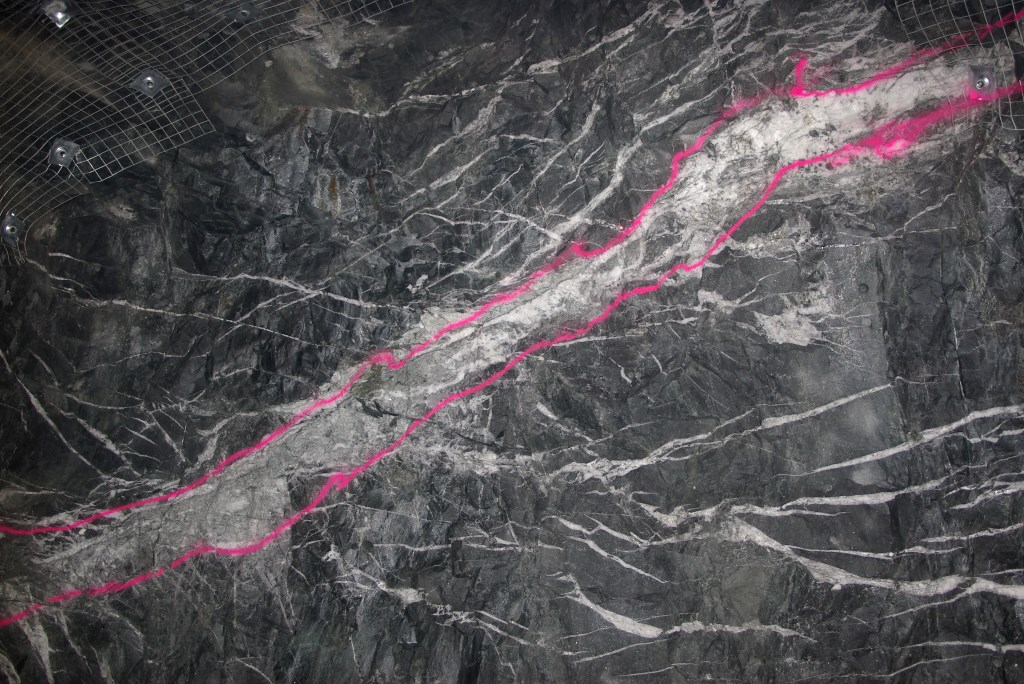
\includegraphics[width=0.6\textwidth]{revisao_bibliografica/veio_ouro.jpg}
	\end{center}
	\legend{Fonte: \url{http://rses.anu.edu.au/people/steve-cox}, acesso em julho de 2016}
\end{figure}
				
Segundo \citeonline{mclennan}, para que a decisão de estacionariedade seja razoável um total de cinco fases devem ser consideradas: 
				
\begin{enumerate}
\item{Escolher o número e tipo dos domínios que terão suas propriedades petrofísicas modeladas;}
\item{Modelar as fronteiras desses domínios;}
\item{Caracterizar a natureza das transições entre os domínios e modelá-las;}
\item{Modelar as tendências (\textit{trends}) dentro de cada domínio;}
\item{Estimar com um modelo de tendência.}
\end{enumerate}
				
A escolha dos domínios deve ser avaliada com base em um equilíbrio entre um modelo geológica e fisicamente consistentes e o número de amostras disponível para inferir os parâmetros das SRF \cite{mclennan}.

Além da imposição matemática, os domínios de um depósito mineral devem ser modelados para que estimativas mais precisas de volume/massa e teores sejam obtidas e problemas de diluição ocasionados pela falta de aderência do modelo de blocos às estruturas geológicas do depósito sejam reduzidos \cite{rasera2014estrati}. 
				
\section{Funções implícitas} \label{sec_func_imp}

Alguns dos métodos determinísticos de modelagem geológica disponíveis, e revisados nessa dissertação, são baseados em funções implícitas. O uso da modelagem implícita foi introduzido no campo da computação gráfica para criação de objetos de diversas geometrias e complexidades por \citeonline{bloomenthal1997introduction}. A ideia central da técnica é usar uma função implícita para demarcar regiões de diferentes formas e extensões no espaço \cite{maureira}.

Na matemática, uma equação implícita é uma relação na forma $R(x_1,...,x_n)=0$. Por exemplo, a equação implícita de um círculo unitário é $x^2+y^2-1=0$.

Uma função implícita é uma função definida implicitamente por uma equação implícita, associando uma das variáveis (o valor) com as outras (os argumentos). A função implícita que define o círculo unitário pode ser escrita como $x^2+f(x)^2-1=0$. Essa equação implícita define $f$ como uma função de $x$ apenas se $-1 \leq x\leq 1$.

Os exemplos a seguir, que ilustram a metodologia, foram propostos por \citeonline{osher}.

Na \autoref{linha}, em uma dimensão, a linha dos números reais foi dividida em três partes distintas usando os pontos $x=-1$ e $x=1$. Isto é, definimos $(-\infty,-1)$, $(-1,1)$ e $(1,\infty)$. A primeira e terceira partes são peças desconexas da mesma região. Assim, definimos $\Omega^-=(-1,1)$ como parte interna do domínio e $\Omega^+=(-\infty,-1)\cup(1,\infty)$ como parte externa do domínio. A fronteira entre a parte interna e externa consiste dos dois pontos $\partial\Omega=\{-1,1\}$, e é chamada de interface. No $\Re^n$, os subdomínios são $n$-dimensionais, enquanto a interface apresenta $n-1$ dimensões.

\begin{figure}[!htb]
	\caption{\label{linha}Linha dos reais dividia em dois subdomínios pelos pontos $x=-1$ e $x=1$.}
	\begin{center}
		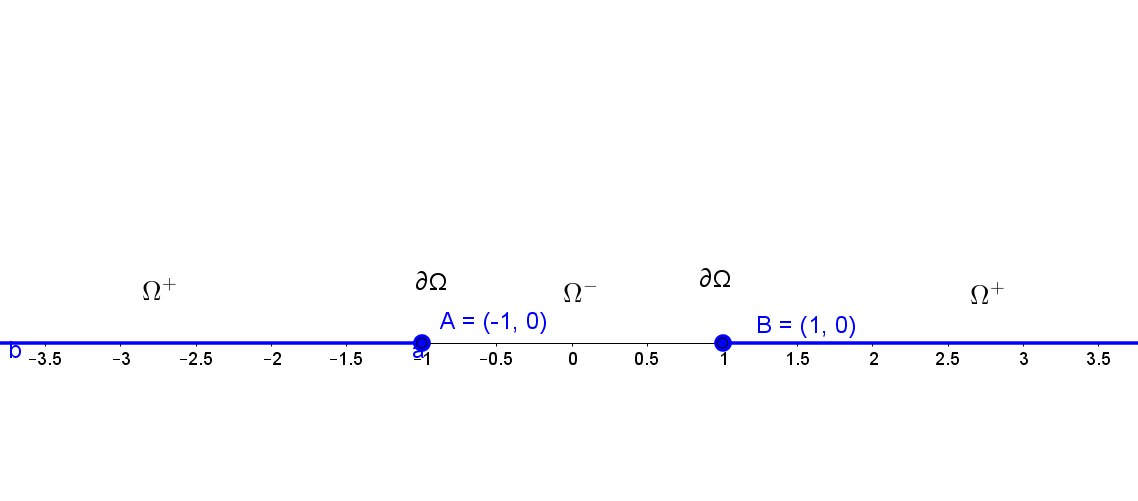
\includegraphics[width=0.6\textwidth]{revisao_bibliografica/linha}
	\end{center}
	%\legend{}
\end{figure}

Numa representação explícita da interface, escrevemos explicitamente os pontos que a definem como feito anteriormente ao definir $\partial\Omega=\{-1,1\}$. Também é possível definir implicitamente a interface como o isocontorno de de alguma função. Por exemplo, o isocontorno zero de $\phi(x)=x^2-1$ é o conjunto de pontos para os quais $\phi(x)=0$, isto é, exatamente $\partial\Omega=\{-1,1\}$, como pode ser observado na \autoref{func}. 

\begin{figure}[!htb]
	\caption{\label{func}Função implícita definindo as regiões $\Omega^-$ e $\Omega^+$ bem como a fronteira $\partial\Omega$.}
	\begin{center}
		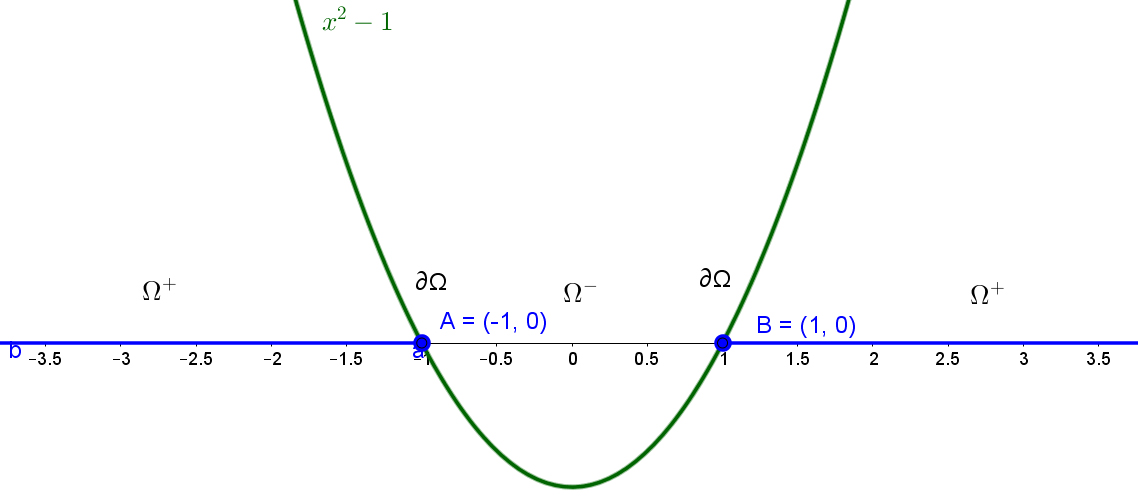
\includegraphics[width=0.6\textwidth]{revisao_bibliografica/funcao}
	\end{center}
	\legend{Modificado de \citeonline{osher}}
\end{figure}

O isocontorno zero foi escolhido. Porém não há nada de especial nessa escolha, o isocontorno $\phi(x)=1$ da função $\phi(x)=x^2$ define a mesma interface.

\subsection{Funções distâncias assinaladas}

Na \autoref{sec_func_imp}, foram definidas as funções implícitas, seu valor é $\phi(x)=0$ na interface, $\phi(x)<0$ na região interna e $\phi(x)>0$ na região externa. As funções distância assinaladas são um subconjunto das funções implícitas.     

Uma função distância $d(\vec{x})$ é definida como:

\begin{equation}
d(\vec{x})=min(|\vec{x}-\vec{x_I}|) \quad \forall \quad \vec{x_I} \in \partial\Omega
\end{equation}

Onde $\vec{x_I}$ é um ponto pertencente à interface. Ou seja, para um dado ponto $\vec{x}$, $d(\vec{x})$ é a menor distância entre $\vec{x}$ e um ponto $\vec{x_C}$ pertencente à interface $\partial\Omega$.   

Uma função distância assinalada é uma função implícita $\phi$, com $|\phi(\vec{x})|=d(\vec{x})$ para todo $\vec{x}$. Então, $\phi(\vec{x})=d(\vec{x})=0$ para todo $\vec{x} \in \partial\Omega$, $\phi(\vec{x})=-d(\vec{x})$ para todo $\vec{x} \in \Omega^-$ e $\phi(\vec{x})=d(\vec{x})$ para todo $\vec{x} \in \Omega^+$.

Na \autoref{sec_func_imp}, a função $\phi(x)=x^2-1$ foi usada para representar implicitamente a interface $\partial\Omega=\{-1,1\}$. Uma representação baseada em funções distância assinaladas da mesma interface é $\phi(x)=|x|-1$, como visto na \autoref{sig_dist} 

\begin{figure}[!htb]
	\caption{\label{sig_dist}Função distância assinalada definindo as regiões $\Omega^-$ e $\Omega^+$ bem como a fronteira $\partial\Omega$.}
	\begin{center}
		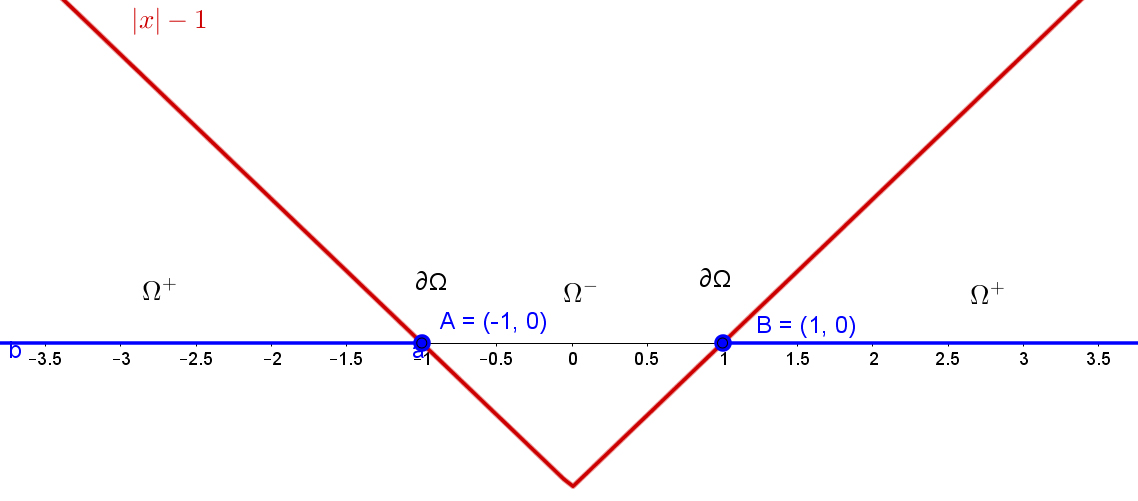
\includegraphics[width=0.6\textwidth]{revisao_bibliografica/signed_dist}
	\end{center}
	\legend{Modificado de \citeonline{osher}}
\end{figure}

Contextualizando, considere o furo de sondagem vertical interceptando uma camada de carvão, à direita na \autoref{carvao}, e o valor da função distância assinalada para essa litologia à esquerda. O valor da função decresce à medida que um ponto ao longo do furo se aproxima da camada, e seu valor é a menor distância desse ponto até um ponto pertencente à interface. Vale zero na interface, e passa a ser negativo para pontos no interior da camada, atingindo o menor valor no centro, parte mais interna da camada de carvão.

\begin{figure}[!htb]
	\caption{\label{carvao}Furo de sonda interceptando uma camada de carvão, à esquerda, e o valor da função distancia assinalada à direita.}
	\begin{center}
		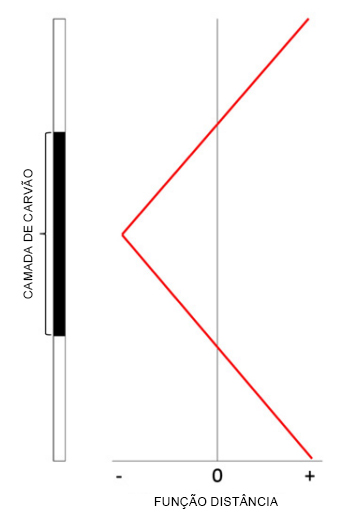
\includegraphics[width=0.2\textwidth]{revisao_bibliografica/carvao}
	\end{center}
	\legend{Modificado de \citeonline{deutschcoal}}
\end{figure}

Os exemplos apresentados são casos simplórios baseados em funções paramétricas e não são aplicáveis a características geológicas, embora a ideia central seja a mesma, algumas adaptações devem ser feitas para o emprego da técnica sob uma perspectiva geológica. A \autoref{metodologia} descreve como as funções implícitas devem ser construídas e aplicadas.

\section{Método implementado no \textit{software} \textit{Leapfrog}\textsuperscript{\textregistered}}\label{sec_leapfrog}

O assunto foi introduzido no campo da geologia por \citeonline{cowan2002rapid,cowan2003practical}, baseado no trabalho de \citeonline{savchenko} para modelar objetos através da interpolação de uma função implícita. 

O \textit{Leapfrog}\textsuperscript{\textregistered} permite a construção de modelos, geológicos e/ou de iso teores (\textit{grade shells}), tridimensionais a partir dos dados brutos de sondagem em questão de minutos ou horas, contra dias ou até semanas gastos com o método tradicional. Desse modo, diferentes cenários geológicos podem ser testados. Os modelos são gerados de forma semi automática. Ademais, informação geológica qualitativa pode ser incorporada ao modelo de forma prática e rápida \cite{cowan2002rapid}.
 
 \subsection{Metodologia}
 
Corpos geológicos são definidos implicitamente a partir dos dados de litologia provenientes da sondagem. O valor de uma função implícita (função distância assinalada ou função volume) é calculado para os pontos amostrais e interpolado para todo o espaço. Então, o volume que representa o corpo geológico é definido por uma iso superfície (geralmente a iso superfície zero) da função implícita interpolada \cite{cowan2003practical}. A metodologia para construção da função distância assinalada é elucidada na \autoref{metodologia}. Os corpos geológicos são modelados individualmente, em ordem geocronológica, do mais recente para o mais antigo, evitando a sobreposição de domínios. O \textit{Leapfrog}\textsuperscript{\textregistered} trabalha convertendo uma função implícita em uma superfície triangulada (\textit{mesh}) que representa a unidade geológica.

\subsubsection{Interpolação}

O exemplo a seguir, que ilustra a metodologia de interpolação implementada no \textit{software}, foi apresentado por \citeonline{leapfrogpredictions}.

\begin{figure}[!htb]
	\caption{\label{dk_amostras}Três amostras $s_1$, $s_2$ e $s_3$ e o um ponto $q$ a ser estimado.}
	\begin{center}
		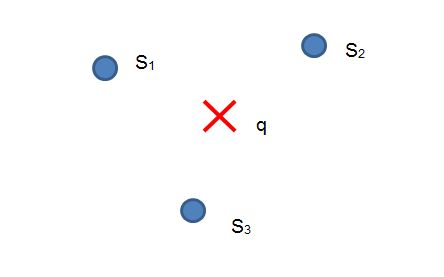
\includegraphics[width=0.4\textwidth]{revisao_bibliografica/dual_krig_amostras}
	\end{center}
	\legend{Fonte: \citeonline{leapfrogpredictions}}
\end{figure}

A \autoref{dk_amostras} ilustra o problema fundamental de estimar o valor $q$ a partir de três amostras $s_1$, $s_2$ e $s_3$.

A krigagem, em sua forma mais simples, estima o valor em um ponto como uma combinação linear das amostras conhecidas, os pesos são determinados matematicamente pela distribuição das amostras em relação ao ponto a ser estimado. Considerando o exemplo anterior:

\begin{equation}
q=w_1s_1+w_2s_2+w_3s_3
\end{equation}

Onde $w_1$, $w_2$ e $w_3$ são os pesos atribuídos às amostras.

Fica evidente que a krigagem pode ser usada como forma de interpolação, já que é possível estimar um valor em qualquer posição arbitrária onde não há dados. Todavia, para cada nova estimativa, é necessário recalcular os pesos, um processo que toma esforço computacional e tempo.

É possível rearranjar a equação de krigagem da seguinte forma:

\begin{equation}
q(x)=a_1\psi(x-x_1)+a_2\psi(x-x_2)+a_3\psi(x-x_3)
\end{equation}

Esse método é conhecido como \textit{dual kriging} \cite{galli1984dual}. $a_1\psi(x-x_1)$ descreve como a amostra localizada na posição $x_1$ influencia a estimativa na sua vizinhança, $\psi(x)$ é equivalente ao variograma (ou interpolante no casos das RBF). Nessa abordagem, as influências ponderadas de cada amostra são somadas para produzir uma equação que possa ser usada para estimar um valor em qualquer local $x$. Uma estimativa feita dessa maneira produz o mesmo resultado do que o método tradicional de krigagem. 

A \autoref{dk_pesos} ilustra um exemplo unidimensional do método

\begin{figure}[!htb]
	\caption{\label{dk_pesos}Demonstração simplificada do funcionamento das funções de bases radiais em uma dimensão.}
	\begin{center}
		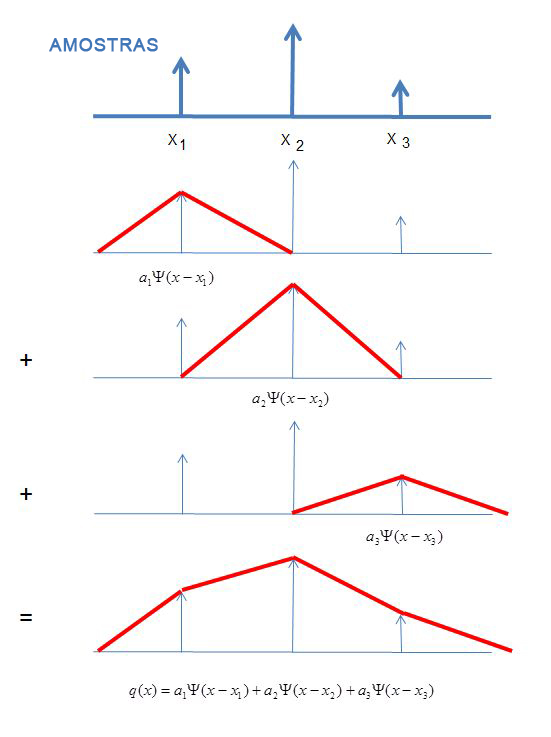
\includegraphics[width=0.4\textwidth]{revisao_bibliografica/dual_krig_pesos}
	\end{center}
	\legend{Modificada de \citeonline{leapfrogpredictions}}
\end{figure}

Utilizando a metodologia tradicional de krigagem, para cada nova estimativa em um local diferente é preciso recalcular os pesos, já com a \textit{dual kriging}, onde a influência das amostras é somada, os pesos só precisam ser calculados uma única vez. Acelerando o processo.

O \textit{Leapfrog}\textsuperscript{\textregistered} usa funções de bases radias (RBF) para interpolar a função distância assinalada retendo todas as amostras disponíveis (estimador global) em todas as estimativas. Mais especificamente \textit{FastRBF}\textsuperscript{TM}, cuja diferença principal em relação à RBF tradicional, é a capacidade de trabalhar com bancos de dados volumosos (mais de 1.000.000 de amostras) em um hardware convencional de forma relativamente rápida \cite{leapfrogfastrbf}. 

RBF são uma forma de implementar a \textit{dual kriging} \cite{leapfrogpredictions}. Enquanto a krigagem usa uma função covariância obtida através dos dados para determinar os pesos dados às amostras, as RBF usam funções básicas (\textit{interpolant functions}) pré-definidas para determiná-la.

Duas funções são usadas para derivar os pesos dados à cada amostra no \textit{Leapfrog}\textsuperscript{\textregistered}, o interpolante linear (\autoref{interpolantes} à esquerda) e o interpolante esferoidal (\autoref{interpolantes} à direita). Equivalentes aos modelos de variograma potência e esférico, respectivamente \citeonline{leapfrogbasics}.

O interpolante linear é multi escala, o que o torna bastante flexível e de uso geral. Particularmente recomendado para casos em que há um grande número de dados de litologia concentrados em bolsões localizados. Não é recomendado para teores, já que extrapola violentamente para além do limite dos dados. O interpolante esferoidal contorna o problema de extrapolação, muitas vezes não realista, do modelo linear \cite{leapfroginterpolant}.Os parâmetros do modelo como patamar, alcance e efeito pepita podem ser ajustados.

\begin{figure}[!htb]
	\caption{\label{interpolantes}Interpolantes do \textit{Leapfrog}\textsuperscript{\textregistered}.}
	\begin{center}
		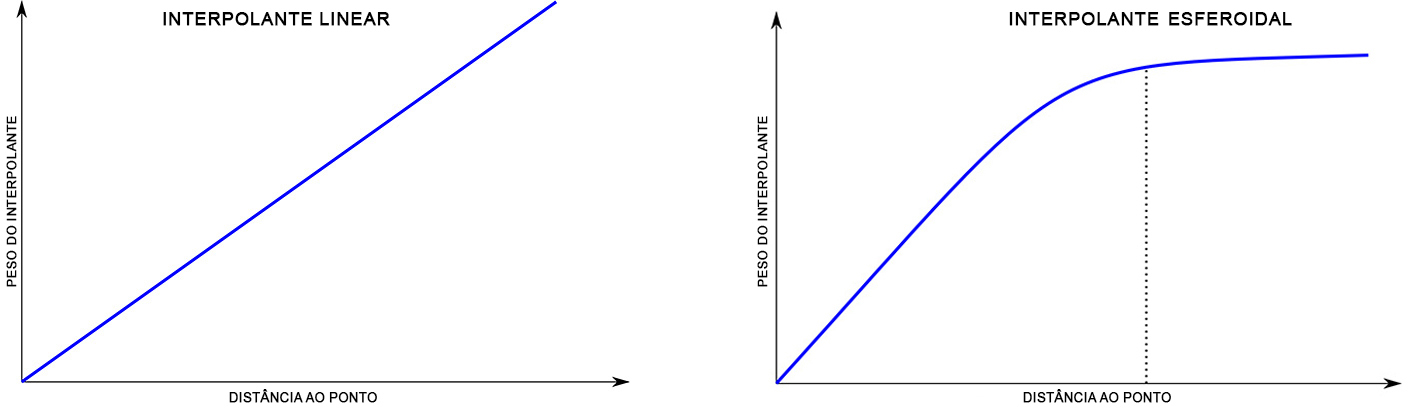
\includegraphics[width=0.8\textwidth]{revisao_bibliografica/interpolantes}
	\end{center}
	\legend{Modificada de \citeonline{leapfrogbasics}}
\end{figure}

\subsubsection{Anisotropia}

O \textit{Leapfrog}\textsuperscript{\textregistered} conta com ferramentas que dão ao usuário controle sobre a continuidade dos corpos geológicos em determinadas direções com possibilidade de incorporar à interpolação uma tendência global e/ou uma tendência estrutural.

A tendência global controla o comportamento do modelo interpolante, e deve ser utilizado em situações onde a geologia sugere continuidade do corpo numa direção planar sobre uma grande área, se a geologia sugerir que a direção dos corpos varia no espaço, a tendência estrutural é mais indicada \cite{leapfroganisglobal}.

A tendência global é inserida ao modelo a partir de um elipsoide de anisotropia, de forma análoga aos variogramas anisotrópicos da geoestatística.

A tendência estrutural é uma generalização da tendência global que permite alterar a direção de continuidade ao longo de uma superfície definida pelo usuário, ao invés de ser baseada em um plano, como a tendência global, definida a partir de um elipsoide de anisotropia. A tendência estrutural é baseada em uma superfície que pode apresentar qualquer forma e orientação, e é condicionada, geralmente, por restrições geológicas, como falhas, dobras, foliações... Para cada ponto da superfície (\textit{mesh}) definida, a tendência local é determinada, produzindo uma anisotropia que varia por todo o espaço definido \cite{leapfrogstructural}.

A tendência estrutural não determina a forma final da unidade geológica, ela é determinada pelo interpolante e pelas amostras retidas na interpolação. A \autoref{isotropico} mostra uma superfície interpolada usando um interpolante isotrópico, a \autoref{global} um interpolante com tendência global e a \autoref{estrutural} um interpolante com tendência estrutural. Todos os sólidos derivam da mesma base de dados.

\begin{figure}[!htb]
	\caption{\label{isotropico}Interpolante isotrópico.}
	\begin{center}
		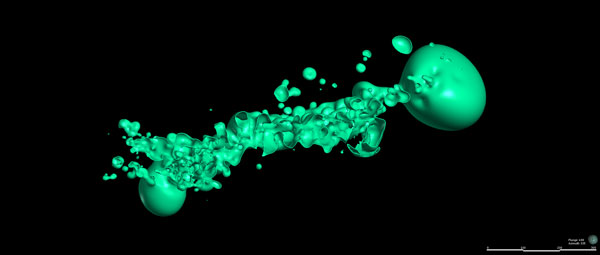
\includegraphics[width=0.5\textwidth]{revisao_bibliografica/isotropic_interpolant}
	\end{center}
	\legend{Fonte: \citeonline{leapfrogstructural}}
\end{figure}

\begin{figure}[!htb]
	\caption{\label{global}Tendência global aplicada ao interpolante.}
	\begin{center}
		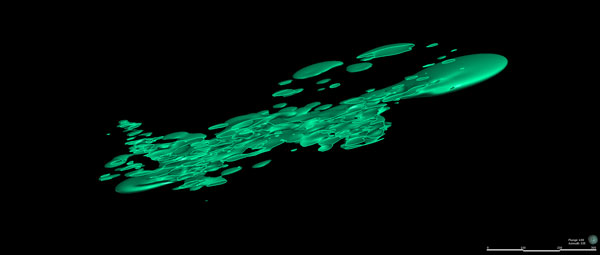
\includegraphics[width=0.5\textwidth]{revisao_bibliografica/global_trend_interpolant}
	\end{center}
	\legend{Fonte: \citeonline{leapfrogstructural}}
\end{figure}

\begin{figure}[!htb]
	\caption{\label{estrutural}Tendência estrutural aplicada ao interpolante.}
	\begin{center}
		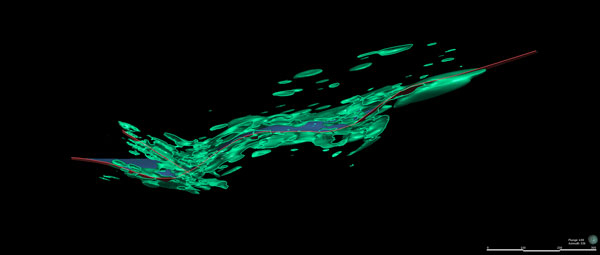
\includegraphics[width=0.5\textwidth]{revisao_bibliografica/structural_trend_interpolant}
	\end{center}
	\legend{Fonte: \citeonline{leapfrogstructural}}
\end{figure}

O \textit{Leapfrog}\textsuperscript{\textregistered} disponibiliza três tipos de tendência estrutural (\textit{non-decaying trends}, \textit{blended trends} e \textit{strongest along meshes}), que compartilham os mesmos parâmetros força (\textit{strength}) e alcance (\textit{range}). A força é semelhante à razão do elipsoide e dita quanta elongação existirá em uma determinada direção. Enquanto o alcance dita até que distância da superfície definida (\textit{mesh}) a tendência ainda tem efeito \cite{leapfrogstructural}.  

\subsubsection{Visão geral}

A metodologia do \textit{Leapfrog}\textsuperscript{\textregistered} compreende cinco passos \cite{cowan2002rapid}:
\begin{enumerate}
\item Validação dos dados e compositagem: Esse passo pode ser executado na maior parte dos software de mineração disponíveis;
\item Interpolação e \textit{meshing}: Extrair iso superfícies de uma função distância assinalada interpolada;
\item Incorporar geomorfologia: estruturas geológicas interpretadas pelo geomodelador são inseridas no modelo como tendência estrutural;
\item Interpolação da informação morfológica: Uma função de interpolação é ajustada à informação digitalizada no passo anterior;
\item Interpolação condicionada à informação geomorfológica: A interpolação do segundo passo é repetida, dessa vez, condicionada pela função de interpolação da informação morfológica gerada no quarto passo. Essa etapa gera modelos que honram os dados amostrais, e são consistentes com a informação qualitativa interpretada pelo geomodelador.
\end{enumerate}

A metodologia implementada no \textit{leapfrog}\textsuperscript{\textregistered} supera muitas das limitações dos métodos explícitos. Os domínios são construídos de forma rápida, o método é objetivo, replicável e nova informação geológica pode ser incorporada facilmente aos modelos. O \textit{software} conta com funções interessantes como a possibilidade de inserir no modelo informação geológica qualitativa e ferramentas específicas para modelar estruturas geológicas complexas como diques. No entanto, o fato da RBF ser um interpolador global pode inviabilizar o uso do método em bancos de dados muito grandes, o método não trabalha com múltiplos domínios de forma direta e sua licença é bastante cara \cite{mclennan2006implicit}.

\section{Método dos campos potenciais}\label{sec_campos}

O método dos campos potenciais, implementado no \textit{software Isatis} \textsuperscript{\textregistered}, foi criado para construir modelos geológicos tridimensionais a partir de dados de geologia e de exploração \cite{chiles2004modelling}. O princípio do método é derivar a geometria dos domínios a partir da interpolação tridimensional de um campo escalar, conhecido como campo potencial. O campo potencial é construído através da cokrigagem da informação dos contatos geológicos provenientes de furos de sondagem e dados estruturais \cite{renard2013modeling}.

A localização dos contatos estabelece a posição de referência de iso valores do campo potencial enquanto os dados de orientação são o gradiente da função escalar (campo potencial). A geometria dos corpos geológicos é obtida a partir da discretização de iso valores de referência \cite{calcagno2008geological}, semelhante a como uma unidade geológica é definida a partir de uma iso superfície de uma função implícita nos métodos apresentados na \autoref{sec_leapfrog} e \autoref{metodologia}. 

A covariância da cokrigagem e o gradiente do campo potencial estimado podem ser transformados em medidas de incerteza da localização da fronteira dos domínios ou usadas para mapear a probabilidade de um local não amostrado pertencer a um determinado domínio geológico \cite{renard2013modeling}.

\subsection{Metodologia}

O método consiste em modelar uma interface geológica ou uma série de interfaces sub paralelas $l_k$, $k=1,2,...$. Seu princípio é sumarizar a geologia a partir de um campo potencial, isto é, uma função escalar $T(p)$ de qualquer ponto $p=(x,y,z)$ no espaço tridimensional, a interface $l_k$ corresponde a uma superfície iso potencial, ou seja, o conjunto de pontos $p$ que satisfazem $T(p)=t_k$ para algum valor desconhecido $t_k$ do campo potencial. De forma análoga, a formação geológica entre duas interfaces sucessivas $l_k$ e $l_{k'}$ é definida por todos os pontos $p$ os quais o campo potencial pertence ao intervalo definido por $t_k$ e $t_{k'}$ \cite{chiles2004modelling}. 

A \autoref{pot_field_1} ilustra o princípio em duas dimensões. À esquerda, uma formação geológica foi mapeada pela posição de suas interfaces com outras duas formações (pontos vermelhos e azuis) e medidas do mergulho (setas). À direita, a formação geológica foi modelada pelo método dos campos potenciais, curvas vermelhas e azuis representam iso valores de referência dos contatos modelados. Curvas brancas são iso valores selecionados do campo potencial, e representam tendências geológicas ou trajetórias de foliações. As interfaces honram tanto os pontos pertencentes aos contatos quanto os vetores de orientação \cite{calcagno2008geological}.

\begin{figure}[!htb]
	\caption{\label{pot_field_1}Princípio do método dos campos potenciais em duas dimensões.}
	\begin{center}
		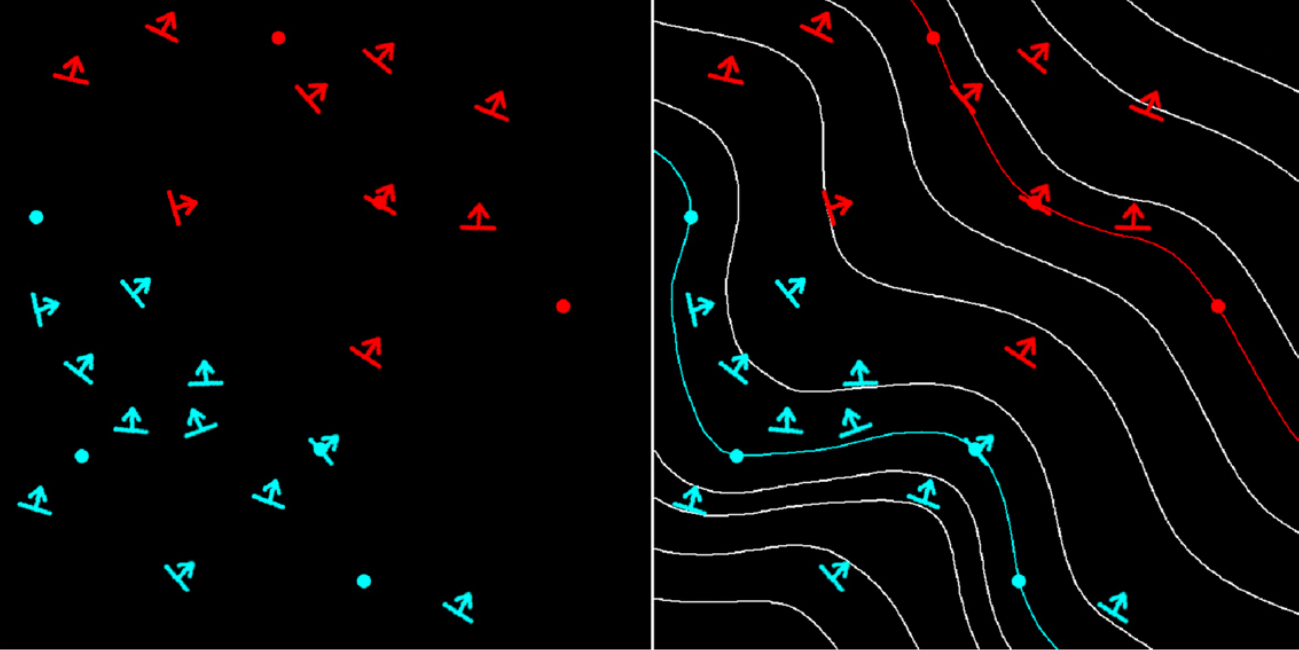
\includegraphics[width=0.8\textwidth]{revisao_bibliografica/pot_field_1}
	\end{center}
	\legend{Fonte: \citeonline{calcagno2008geological}}
\end{figure}

\subsection{Tipos de dados}

$T(p)$ é modelada com dois tipos diferentes de dados \cite{chiles2004modelling}:

\begin{enumerate}
\item Coordenadas tridimensionais de pontos que pertencem às interfaces $l_1, l_2, ...$ (contatos geológicos);
\item Vetores unitários tridimensionais que pertencem ao campo de orientação das interfaces.  
\end{enumerate}

Na modelagem tridimensional de interfaces sedimentares, a informação estrutural consiste em vetores unitários ortogonais ao principal plano de anisotropia (acamamento, xistosidade, foliação) e apontando no sentido das formações mais jovens. Na modelagem de um domínio mineralizado, os vetores unitários apontam do interior para o exterior dos domínios \cite{renard2013modeling}.

\subsubsection{Codificação dos dados}

Para interpolar o campo potencial, os dados devem ser codificados da seguinte forma \cite{chiles2004modelling, calcagno2008geological, renard2013modeling}:


\begin{enumerate}
\item Pontos da interface: O valor potencial $c$ associado com a interface não é conhecido, mas a diferença potencial entre dois pontos de uma interface é igual a zero (já que as superfícies são equipotenciais). Os $m+1$ pontos $p_0, p_1, ..., p_m$ da interface são transladados em $m$ incrementos $T(p_{\alpha})-T(p'_\alpha)=0$, $\alpha=1,...,m$. $p'_\alpha$ pode ser tanto o ponto $p_0$ ou o ponto $p_{\alpha-1}$ (a escolha não tem impacto no resultado);
\item Dados de orientação: Os vetores unitários normais a cada plano estrutural, são considerados como gradiente do campo potencial, equivalentes ao valor da derivada parcial $\frac{\partial T(p)}{\partial u}$ no ponto medido $p_\beta$ em qualquer direção $u$. O dado estrutural em $p_\beta$ pode ser escrito como três derivadas parciais da forma $\frac{\partial T(p_\beta)}{\partial u_\beta}$, $u_\beta$, representando os eixos de coordenadas $x, y, z$ (um outro conjunto de derivadas parciais em três direções ortogonais também pode ser considerado. Por exemplo, o vetor unitário pode ser expressado por uma derivada parcial igual a um na direção do vetor, e duas derivadas parciais iguais a zero nas direções que definem o plano estrutural).    
\end{enumerate}

\subsubsection{Interpolação do campo potencial}

A função potencial $T(.)$ é definida até uma constante arbitrária que é o potencial em um ponto de referência arbitrário $p_0$. Em cada ponto $p$ o incremento do campo potencial $T(p)-T(p_0)$ é krigado. O estimador de cokrigagem é escrito como:

\begin{equation}
	\label{eq_pot_field}
    T^*(p)-T^*(p_0)=\sum\limits_{\alpha=1}^M \mu_\alpha(T(p_\alpha)-T(p'_\alpha))+\sum\limits_{\beta=1}^N \nu_\beta \frac{\partial T(p_\beta)}{\partial u_\beta}
\end{equation}

Onde os pesos $\mu_\alpha$ e $\nu_\beta$, determinados pelo sistema de cokrigaem, são função de $p$ (e $p_0$). Embora a contribuição dos incrementos potenciais seja zero, os pesos $\nu_\beta$ são diferentes dos pesos baseados apenas nos dados de gradiente.

A cokrigagem é estabelecida sob o modelo de função aleatória (\autoref{func_al}). $T(.)$ é assumido como uma função aleatória com deriva (\textit{drift}) polinomial $m(p)$:

\begin{equation}
	\label{eq_poli_drift}
    m(p)=\sum\limits_{l=0}^L b_lf^l(p)
\end{equation}

E uma variância estacionária $K(h)$ \cite{calcagno2008geological,renard2013modeling}. Uma vez que as funções básicas $f^l(p)$ da deriva e a covariância $K(h)$ de $T(.)$ sejam conhecidas, a cokrigagem, na presença de dados do gradiente, pode ser calculada. Já que a derivada de $\frac{\partial T(p)}{\partial u}$ vale $\frac{\partial m(p)}{\partial u}$, isto é, uma combinação linear das derivadas parciais $\frac{\partial f^l(p)}{\partial u}$ com os mesmos coeficientes desconhecidos $b_l$ de $m(p)$. As covariâncias das derivadas parciais são derivadas parciais de segunda ordem de $K(.)$, e as covariâncias cruzadas entre campo potencial e as derivadas parciais são derivadas parciais de $K(.)$ \cite{chiles2004modelling}.

\subsubsection{Implementação do algoritmo de cokrigagem}

O incremento dos dados potenciais não contribuem com as estimativas finais. O estimador pode ser visto como integração dos dados de gradiente \cite{chiles2004modelling}. Para garantir a continuidade espacial do estimador, é usada apenas uma vizinhança incluindo todos os dados. Quando não há interesse na variância, a cokrigagem é implementada em sua forma \textit{dual} (\textit{dual kriging}), assim, o sistema de krigagem é resolvido uma única vez. 

$T^*(p)-T^*(p_0)$ pode ser obtido em qualquer ponto. Seu sinal indica onde $p$ está localizado, negativo para formações mais antigas, positivo para formações mais recentes e zero para a interface. Essa propriedade permite a visualização em três dimensões do modelo geológico a partir de um algoritmo de cubos marchantes (\textit{marching cubes}) \cite{lorensen1987marching}, que rastreia a iso superfície do campo potencial \cite{calcagno2008geological}.

\subsubsection{Variância do campo potencial}

Na geoestatística, a covariância ou variograma de uma variável são modeladas a partir dos dados. Porém, não há medidas do potencial $T(x)$, e os incrementos potenciais usados na interpolação não podem ser usados na inferência de $K$, já que todos valem zero.

Na sua primeira implementação, o algoritmo era baseado em um modelo de covariância arbitrariamente escolhido pelo usuário \cite{chiles2004modelling}.

Quando existem muitos dados estruturais disponíveis, o variograma das derivadas parciais pode ser calculado. Os variogramas das derivadas parciais são derivadas de segunda ordem do variograma do campo potencial. \citeonline{renard2013modeling} recomenda que uma soma de modelos anisotrópicos cúbicos de covariância sejam adotados para modelar a covariância.

\subsubsection{Incerteza nos modelos}

Uma formação geológica definida pelo conjunto de pontos $p$ tais que $T(p)-T(p_0)$ está compreendido entre os dois valores $t$ e $t'$. Sob a suposição de que o campo potencial é uma função aleatória gaussiana, a probabilidade de um dado ponto $p$ pertencer à essa formação é:

\begin{equation}
\begin{gathered}
 P\{t \leq T(p)-T(p_0) < t'\}= \\ 
 G\left(\frac{t'-(T^*(p)-T^*(p_0))}{\sigma_{CK}(p)} \right) - G\left(\frac{t-(T^*(p)-T^*(p_0))}{\sigma_{CK}(p)} \right)
\end{gathered}
\end{equation}

Onde G é a função de distribuição acumulada normal.

De forma análoga, para a interface que passa por $p_0$ 

\begin{equation}
	R(p) = T(p)-T(p_0)=\frac{T^*(p)-T^*(p_0)}{\sigma_{CK}}
\end{equation}

Mede a probabilidade de $p$ pertencer à interface.

\subsubsection{Visão geral}

A metodologia compreende cinco passos \cite{mclennan2006implicit}:

\begin{enumerate}
\item Coletar dados de interseção e dados de orientação em superfície;
\item Determinar a forma da deriva (\textit{drift}) localmente variável;
\item Inferir a função covariância do campo potencial;
\item Interpolar o campo potencial com cokrigagem;
\item Visualizar a incerteza na localização das fronteiras estimadas.
\end{enumerate}

O método ainda permite a incorporação de falhas e informação geofísica. É um método flexível, que incorpora uma gama de dados diferentes na modelagem dos domínios geológicos. É rápido, em comparação com os métodos explícitos, é objetivo e replicável. Capaz de produzir modelos bastante complexos como o da \autoref{pot_field_ex}. Porém, o procedimento não é simples. É difícil inferir a covariância dos campos potenciais já que não existem dados amostrais do campo. As medições de orientações nem sempre existem ou são de fácil obtenção. O método etá implementado apenas em software pago.

\begin{figure}[!htb]
	\caption{\label{pot_field_ex}Modelo geológico criado a partir do método dos campos potenciais, em planta (acima). Seção N6 (abaixo).}
	\begin{center}
		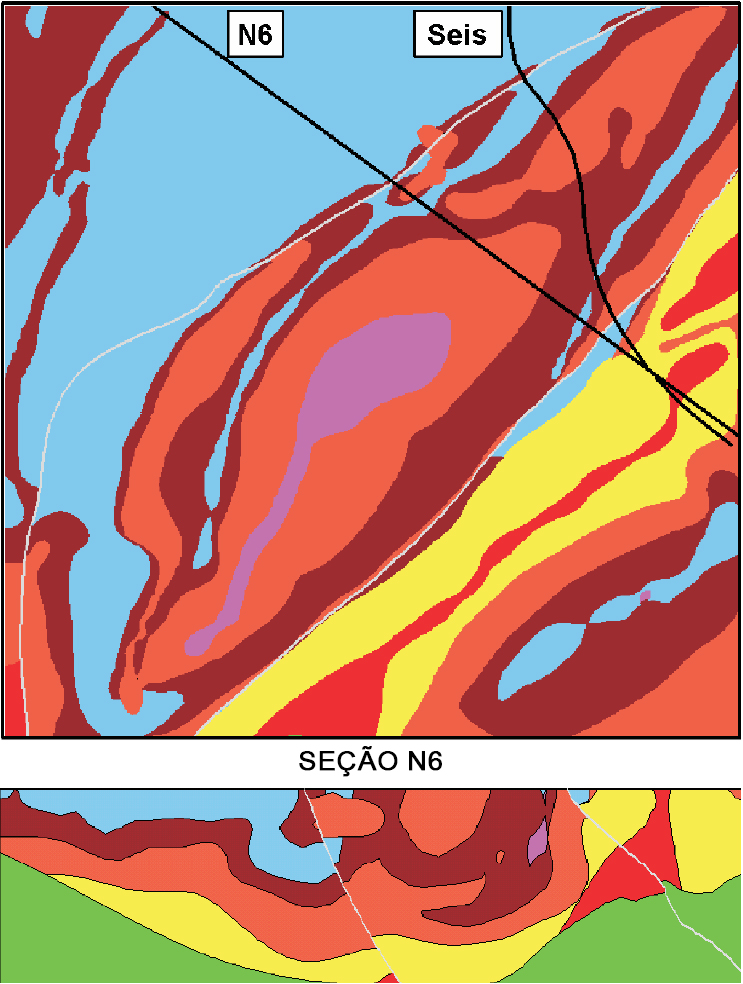
\includegraphics[width=0.5\textwidth]{revisao_bibliografica/pot_field_ex}
	\end{center}
	\legend{Fonte: \citeonline{chiles2004modelling}}
\end{figure}
\chapter{Modelagem geológica implícita com funções distância assinaladas} \label{metodologia}

O método é baseado na interpolação de uma função implícita calculada para cada amostra e posterior definição de uma superfície de iso valores da função interpolada. A cada amostra é atribuída a distância euclideana anisotrópica entre ela mesma e a amostra mais próxima que pertence a um outro domínio geológico. O sinal da distância calculada revela se a amostra se encontra no interior (sinal negativo) ou exterior (sinal positivo) do domínio a ser modelado. A interpolação dessas medidas de distância permite a construção de um modelo binário de domínio geológico aplicando uma regra de corte (valor zero) na função implícita interpolada \cite{silvaanddeutschccgmodeling}. 

Ao contrário dos métodos visitados nas \autoref{sec_leapfrog} e \autoref{sec_campos}, que permitiam a modelagem de um domínio por vez, esse método permite modelar múltiplos domínios simultaneamente. Sendo assim, a categoria correspondente a menor distância estimada deve ser retida.

\section{Metodologia}\label{metodologia}

\subsection{Caso binário}\label{binario}

Primeiramente, o conjunto de dados ${z(u_\alpha),\alpha=1,...,n}$ é codificado em indicadores binários de acordo com a \autoref{eq_ind}, especificando se a amostra pertence ou não ao domínio. 

\begin{equation}
	i(u_\alpha)=\begin{cases}
	1,\:\textrm{se}\:z(u_\alpha)\:\textrm{se pertence ao domínio}\\
	0,\:\textrm{se}\:z(u_\alpha)\:\textrm{caso contrário}\end{cases}
    \label{eq_ind}
\end{equation}

\citeonline{maureira} apresentou um exemplo simples em duas dimensões para ilustrar o método. Na \autoref{indicadores} os pontos amostrais foram codificados em indicadores.

\begin{figure}[!ht]
	\caption{\label{indicadores}Transformação do banco de dados categóricos em indicadores binários.}
	\begin{center}
		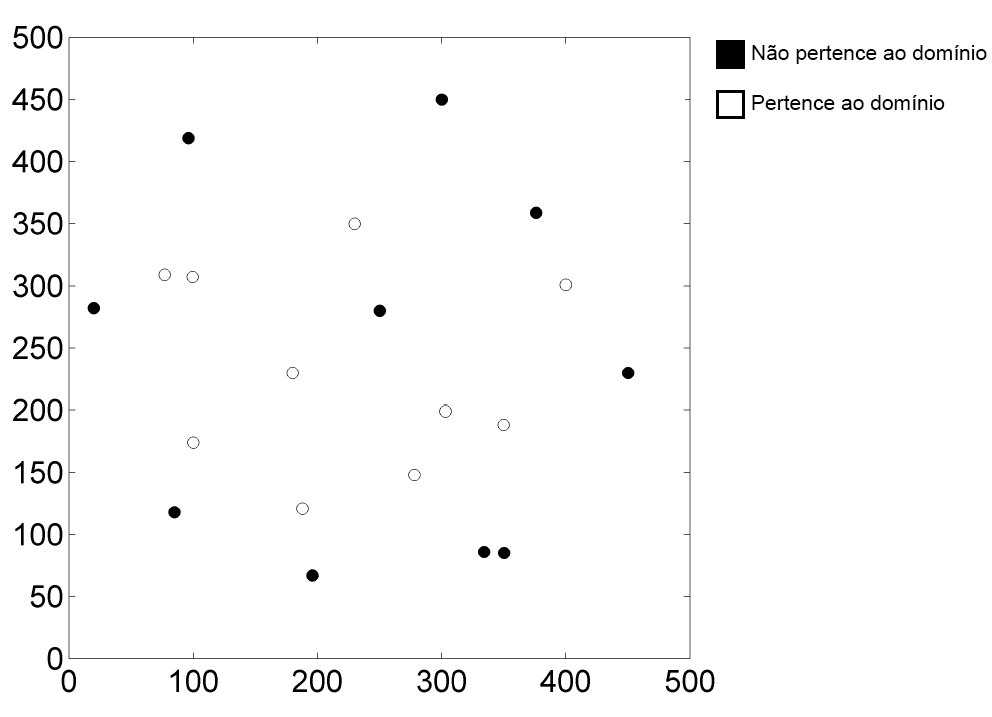
\includegraphics[width=0.5\textwidth]{modelagem_geologica/indicadores}
	\end{center}
	\legend{Fonte: Modificado de \citeonline{maureira}}
\end{figure}

Então, as distâncias assinaladas são calculadas para cada amostra de acordo com a \autoref{eq_sg}. Se a amostra pertence ao domínio modelado a distância é negativa, caso contrário positiva.

\begin{equation}
	d(u_\alpha)=\begin{cases}
	-\parallel u_\alpha-u_\beta\parallel,\:\textrm{se}\:i(u_\alpha)=1\\
	+\parallel u_\alpha-u_\beta\parallel,\:\textrm{se}\:i(u_\alpha)=0\end{cases}
    \label{eq_sg}
\end{equation}

O local $u_\beta$ corresponde à amostra mais próxima que pertença a um domínio diferente de $u_\alpha$. A regra euclideana é usada no cálculo.

A \autoref{distancias} mostra as distâncias assinaladas calculadas para cada ponto amostral.

\begin{figure}[!ht]
	\caption{\label{distancias}Função distância assinalada calculada para cada ponto amostral.}
	\begin{center}
		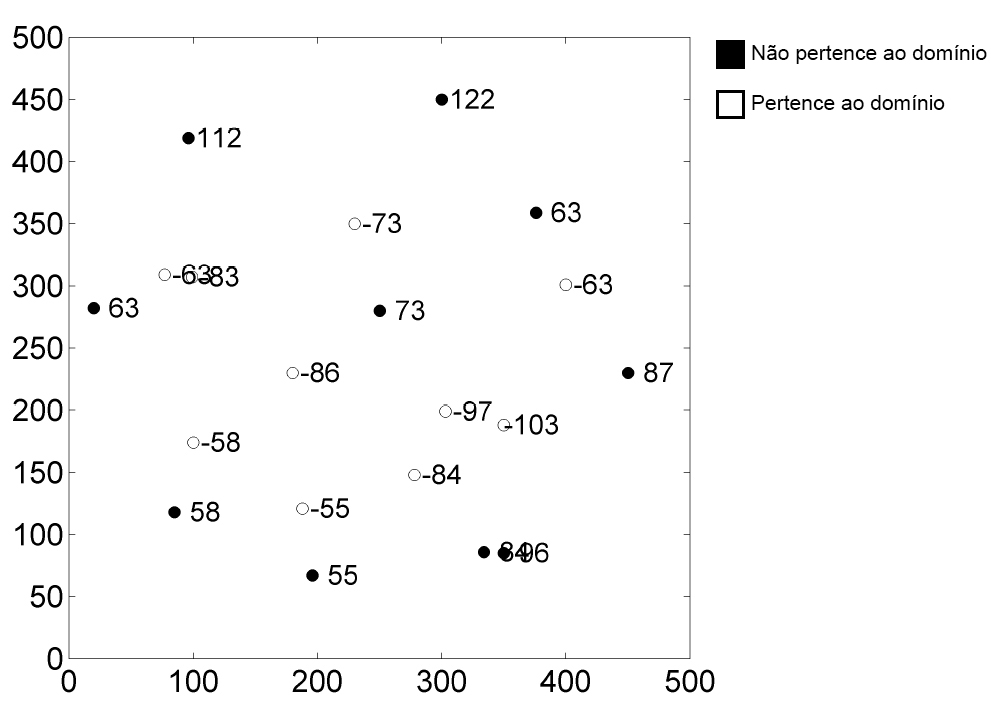
\includegraphics[width=0.5\textwidth]{modelagem_geologica/SG}
	\end{center}
	\legend{Fonte: Modificado de \citeonline{maureira}}
\end{figure}

Nos casos em que há o conhecimento de que o corpo geológico se estende mais em uma direção do que nas outras (como os corpos tabulares, por exemplo) as distâncias calculadas podem ser anisotrópicas. Assim sendo, as coordenadas originais $x$, $y$ e $z$ dos dados devem ser rotacionadas e/ou contraídas/dilatadas, a partir da transformação da \autoref{eq_rot_matrix}. Então, as distâncias euclideanas (\autoref{eq_sg}) são calculadas normalmente para as novas coordenadas $x''$, $y''$, $z''$.

\begin{equation}
\begin{gathered}
\begin{bmatrix} x'' \\ y'' \\ z'' \end{bmatrix} = \begin{bmatrix} \frac{1}{a_{max}} & 0 & 0 \\ 0 & \frac{1}{a_{min}} & 0 \\ 0 & 0 & \frac{1}{a_{vert}} \end{bmatrix} \\ \begin{bmatrix}\cos\alpha\cos\phi-\sin\alpha\sin\beta\sin\phi & -\sin\alpha\cos\phi-\cos\alpha\sin\beta\sin\phi & \cos\beta\sin\phi \\ \sin\alpha\cos\beta & \cos\alpha\cos\beta & \sin\beta \\ -\cos\alpha\sin\phi-\sin\alpha\sin\beta\cos\phi & \sin\alpha\sin\phi-\cos\alpha\sin\beta\cos\phi & \cos\beta\cos\phi \end{bmatrix} \begin{bmatrix} x \\ y \\ z \end{bmatrix}
\end{gathered}
	\label{eq_rot_matrix}
\end{equation}

Onde $a_{max}$, $a_{min}$ e $a_{vert}$ são as dimensões dos eixos máximo, médio e mínimo de anisotropia, e $\alpha$, $\beta$ e $\phi$, os ângulos de azimute, mergulho e \textit{rake}, respectivamente.   

A construção da função implícita em cada ponto amostral é a mesma para o método visitado na \autoref{sec_leapfrog}.

A função distância calculada para cada amostra é então interpolada para todos os pontos de interesse, a partir da \autoref{eq_OK}. Qualquer técnica de interpolação pode ser utilizada. Inverso da distância e krigagem produzem limites realísticos para os domínios. Porém, a krigagem permite levar em consideração a anisotropia e continuidade espacial das distâncias calculadas \cite{silvaanddeutschccgmodeling}.

\citeonline{silvaanddeutschccgmodeling,deutschcoal,maureira} recomendam que a krigagem global \cite{neufeld}, um interpolador suave que retém todas as amostras nas estimativas (não há estratégia de busca), seja utilizada. Desse modo, evita-se o surgimento de artefatos nos mapas gerados. Todavia, reter todas as amostras na interpolação pode aumentar consideravelmente o tempo de execução do algoritmo. Testes realizados no \autoref{estudo_de_caso} mostraram que o uso da krigagem ordinária com uma vizinhança de busca e número de amostras retidas suficientemente grandes, produzem um resultado muito semelhante à krigagem global.

\begin{equation}
	d^*(u)=\sum\limits_{\alpha=1}^n \lambda_\alpha^{OK}(u)d(u_\alpha)
    \label{eq_OK}
\end{equation}

Onde $d^*(u)$ é a distância estimada para cada local não amostrado $u$, $\lambda_\alpha^{OK}(u)$ os pesos de krigagem ordinária e $d(u_\alpha)$ o valor da função distância assinalada calculado para cada amostra.

A \autoref{interpolated} mostra a função distância interpolada por krigagem ordinária em todos os pontos de interesse.

\begin{figure}[!ht]
	\caption{\label{interpolated}Função distância interpolada para todos os locais de interesse.}
	\begin{center}
		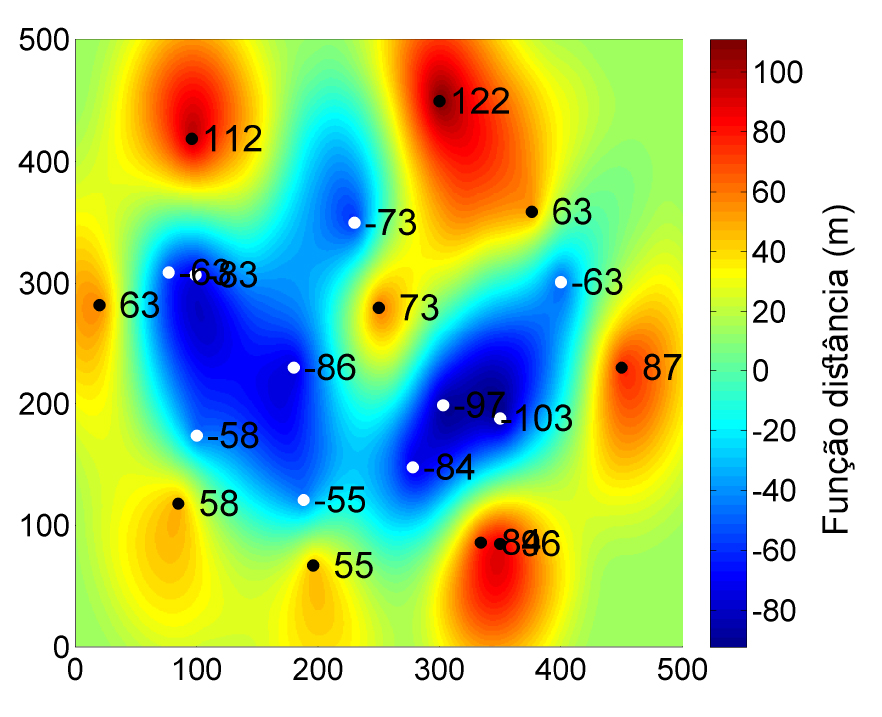
\includegraphics[width=0.5\textwidth]{modelagem_geologica/interpolated}
	\end{center}
	\legend{Fonte: Modificado de \citeonline{maureira}}
\end{figure}

Por fim, cada local de interesse é classificado com base no sinal da função distância interpolada, de acordo com a \autoref{classifier}. Blocos em que a função tem valor negativo, são classificados como pertencentes ao domínio. Blocos em que a função tem valor positivo, classificados como não pertencentes ao domínio.

Como as funções distância são negativas no interior do domínio e positivas no exterior, um bom palpite inicial para a interface que separa os domínios no espaço, seria a linha (em duas dimensões) ou superfície (em três dimensões) que corresponda ao valor zero da função distância assinalada \cite{wildedeutschcalibrate}. 

\begin{equation}
	i^*(u)=\begin{cases}
	1,\:\textrm{se}\:d^*(u)\leq0\\
	0,\:\textrm{caso contrário}\end{cases}
    \label{classifier}
\end{equation}

A \autoref{model} mostra o modelo geológico criado para o domínio a partir do sinal da função distância interpolada (\autoref{interpolated}).

\begin{figure}[!ht]
	\caption{\label{model}Modelo geológico criado a partir do sinal da função distância interpolada.}
	\begin{center}
		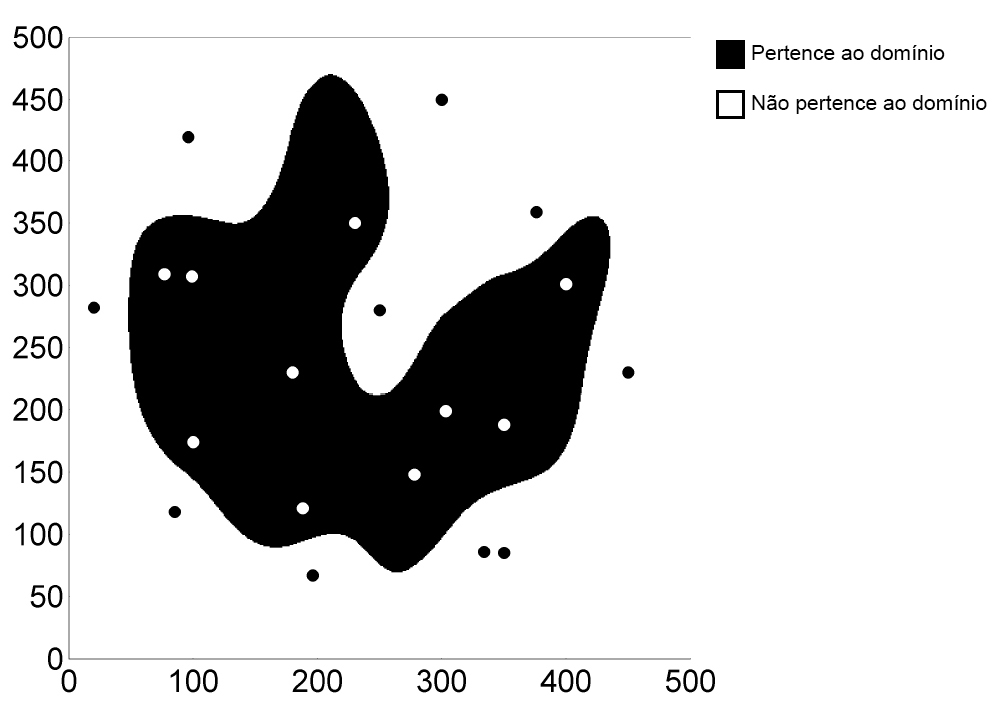
\includegraphics[width=0.5\textwidth]{modelagem_geologica/modelo}
	\end{center}
	\legend{Fonte: Modificado de \citeonline{maureira}}
\end{figure}

\subsection{Aplicação da metodologia para múltiplos domínios geológicos}

A metodologia apresentada na \autoref{binario} é adequada apenas para casos binários, na presença de múltiplas categorias \citeonline{silvaanddeutschccgmodeling} propuseram, também, uma metodologia. O objetivo é modelar os diversos domínios geológicos simultaneamente de forma similar ao caso binário.

Se existirem $K$ múltiplos domínios no depósito mineral, para cada ponto amostral ${z(u_\alpha),\alpha=1,...,n}$, um vetor de indicadores de $K$ elementos é codificado de acordo com a \autoref{eq_mult_ind}.

\begin{equation}
	i_k(u_\alpha)=\begin{cases}
	1,\:\textrm{se}\:z(u_\alpha)=k\\
    0,\:\textrm{se}\:z(u_\alpha)\:\textrm{caso contrário}\end{cases} k=1,...,K
    \label{eq_mult_ind}
\end{equation}

As amostras são codificadas $K$ vezes, uma vez para cada domínio.

Da mesma forma que na \autoref{eq_sg}, a função distância é calculada, individualmente para cada elemento $k$ do vetor, de acordo com a \autoref{eq_mult_sg}.

\begin{equation}
	d_k(u_\alpha)=\begin{cases}
	-\parallel u_\alpha-u_\beta\parallel,\:\textrm{se}\:i_k(u_\alpha)=1\\
	+\parallel u_\alpha-u_\beta\parallel,\:\textrm{se}\:i_k(u_\alpha)=0\end{cases} k=1,...,K
    \label{eq_mult_sg}
\end{equation}

Diferentes anisotropias podem ser incorporadas para cada categoria, a correlação entre as distâncias calculadas não é considerada.

As distâncias calculadas são então interpoladas, individualmente, para cada categoria, de acordo com a \autoref{eq_mult_ok}.

\begin{equation}
	d_k^*(u)=\sum\limits_{\alpha=1}^n \lambda_\alpha^{OK}(u)d_k(u_\alpha)\quad k=1,...,K
    \label{eq_mult_ok}
\end{equation}

Quando os múltiplos variogramas são similares, um único modelo pode se considerado.

Por fim, cada bloco é  classificado pela \autoref{eq_mult_rt}

\begin{equation}
	i^*(u)=k'\;\text{de modo que}\;d_{k'}^*=min\{d_k^*(u)\}_{k=1}^K
    \label{eq_mult_rt}
\end{equation}

As distâncias estimadas fornecem uma medida de proximidade ao domínio oposto mais próximo. Sendo assim, a mínima distância assinalada estimada é tida como o domínio mais provável de ser encontrado numa região não amostrada. A \autoref{eq_mult_rt} sumariza essa ideia \cite{maureira}. A categoria associada com a menor distância estimada é carimbada em cada bloco.

A \autoref{mult_cat} mostra um exemplo de um modelo geológico criado a partir da mínima distância assinalada estimada. A esquerda, a figura mostra a projeção das distâncias assinaladas para cada uma das quatro categorias, e à direita a classificação final.

\begin{figure}[!ht]
	\caption{\label{mult_cat}Função distância interpolada para todos os locais de interesse.}
	\begin{center}
		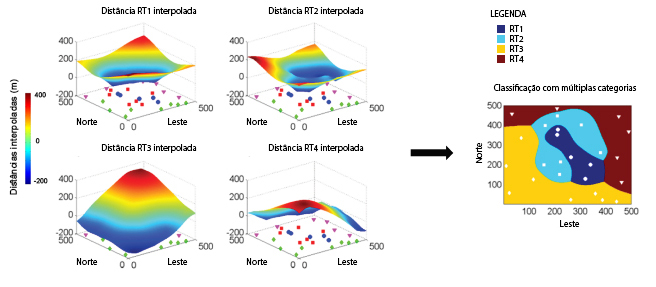
\includegraphics[width=0.8\textwidth]{modelagem_geologica/mult_cat_legenda}
	\end{center}
	\legend{Fonte: Modificado de \citeonline{silvageostatlessons}}
\end{figure}

\section{Uma medida heurística de incerteza (\textit{softmax transformation})}\label{softmax_chap}

A metodologia proposta por \citeonline{silvaanddeutschccgmodeling} não caracteriza a incerteza associada ao modelo geológico. \citeonline{maureira} apresentou uma forma heurística para determinação da incerteza, essa metodologia não é baseada em múltiplas realizações de uma função aleatória, é um pós processamento derivado de uma transformação.

Várias formas de determinar a incerteza para métodos determinísticos de modelagem geológica implícita foram desenvolvidos. \citeonline{mclennan2006implicit} propuseram uma metodologia para quantificar a incerteza de volumes geológicos criados a partir de funções volume (muito similares às funções distância assinaladas) a partir da técnica de \textit{bootstrap sampling}. \citeonline{munroe2012methodology} propôs calibrar uma banda de incerteza ao longo dos contatos entre os domínios, uma ideia similar foi implementada por \citeonline{wildedeutschcalibrate}, onde a incerteza é considerada diretamente na krigagem, adicionando uma constante às estimativas.

As distâncias estimadas em cada bloco para cada categoria carregam consigo informação adicional. Como já discutido, as distâncias estimadas fornecem uma medida de proximidade à interface mais próxima. Então, as distâncias podem ser estandardizadas entre zero e um, fornecendo uma medida de incerteza \cite{maureira}.

\subsubsection{Transformação das distâncias}

\textit{Softmax transformation} é uma técnica amplamente usada em métodos de classificação para múltiplas classes \cite{mccullagh}. A ideia é transformar as distâncias estimadas em probabilidades a partir da \autoref{eq_softmax}. Os valores transformados encontram-se entre zero e um e  sua soma deve ser igual a um, para cada bloco estimado.

\begin{equation}
	P(i(u)=k)=\frac{e^\frac{-d^*_k(u)}{\gamma}}{\sum_{k'=1}^{K}e^\frac{-d^*_k(u)}{\gamma}}
    \label{eq_softmax}
\end{equation}

$P(i(u)=k)$ representa a probabilidade de um local $u$ pertencer à categoria $k$, $d^*_k(u)$ é a distância estimada para a categoria $k$ e $\gamma$ é um parâmetro que regula a inter-relação entre as probabilidades das $K$ diferentes categorias. Quanto maior $\gamma$, maior as diferenças entre as probabilidades (maior a banda de incerteza), como pode ser observado na \autoref{softmax_gamma}.

\begin{figure}[!ht]
	\caption{\label{softmax_gamma}Mapas de probabilidades gerados com dois valores de gamma diferentes. À esquerda $\gamma=80$, à direita $\gamma=175$.}
	\begin{center}
		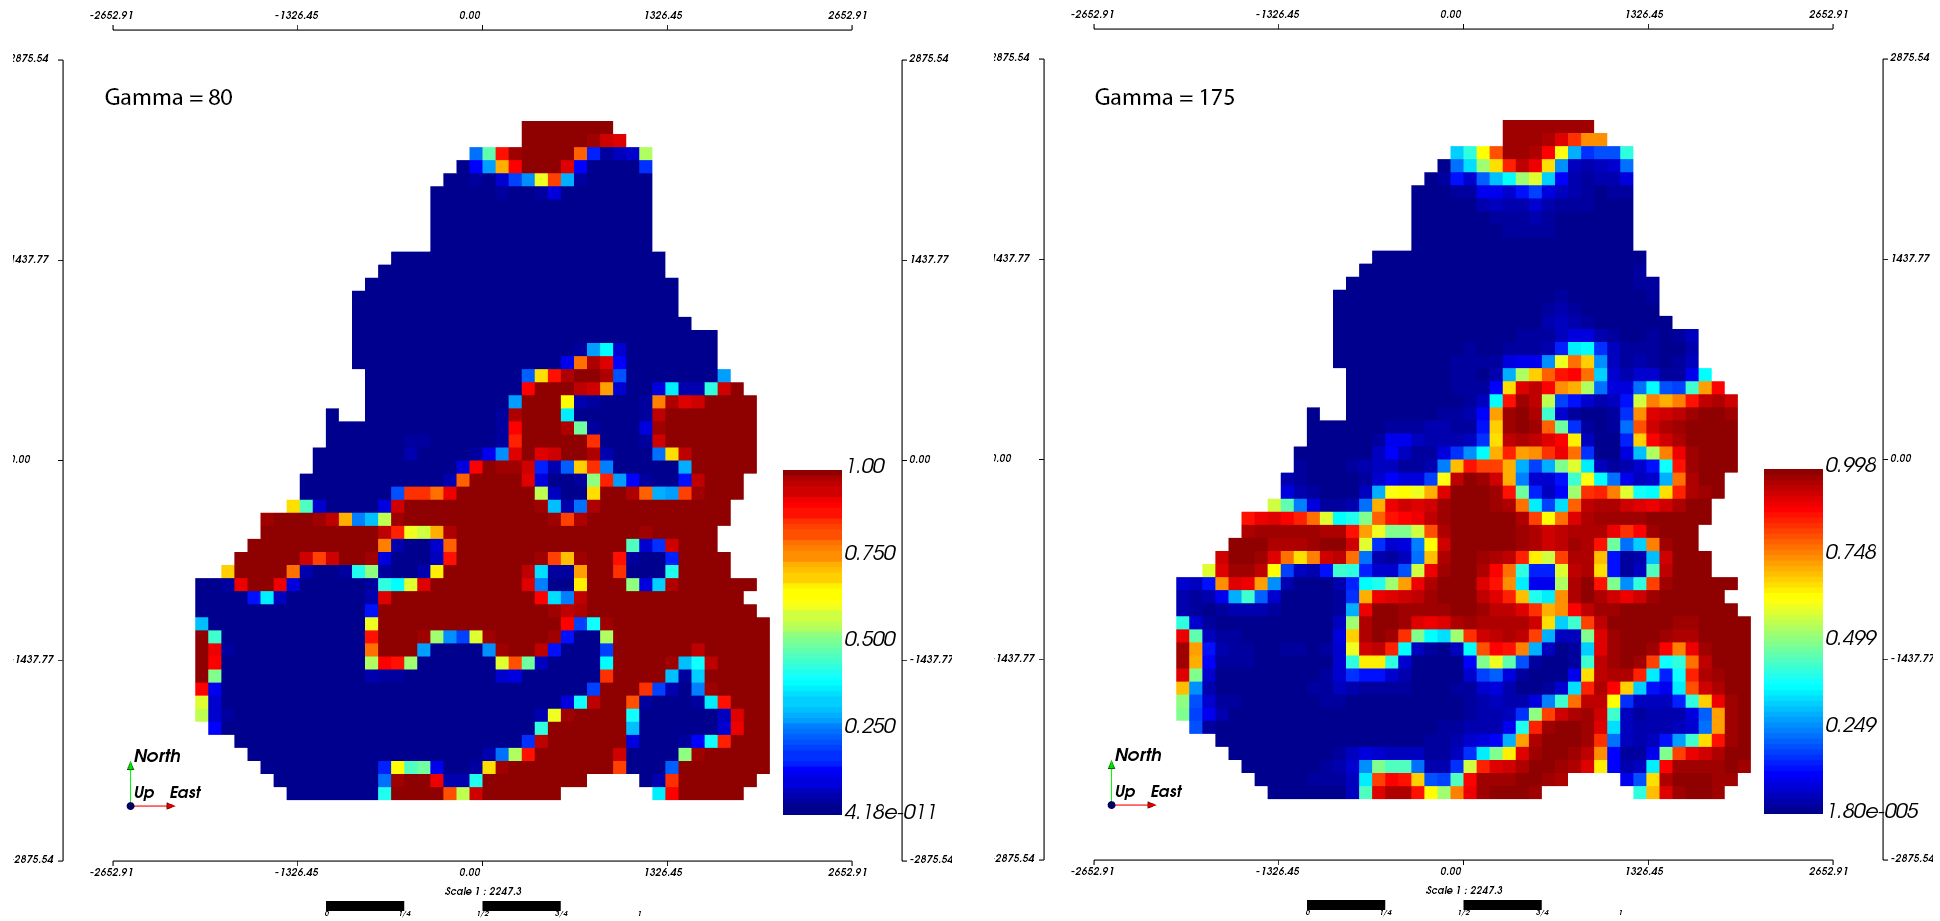
\includegraphics[width=0.6\textwidth]{modelagem_geologica/softmax_gama}
	\end{center}
	%\legend{Fonte: Modificado de \citeonline{maureira}}
\end{figure}

Para exemplificar a transformação, a \autoref{softmax_grafico}, mostra à esquerda as distâncias estimadas para cada uma de cinco categorias em um mesmo bloco em particular. À direita as distâncias transformadas pela \autoref{eq_softmax} em probabilidades daquele bloco pertencer a cada uma das cinco categorias. Observe que distâncias menores (mais negativas) geram probabilidades maiores, e vice-versa.  

\begin{figure}[!ht]
	\caption{\label{softmax_grafico}Distâncias estimadas e transformadas em probabilidades para um mesmo bloco.}
	\begin{center}
		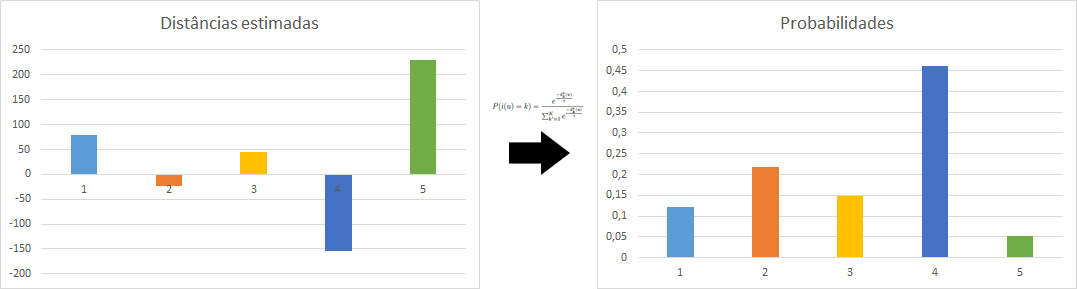
\includegraphics[width=0.7\textwidth]{modelagem_geologica/softmax_bars_final}
	\end{center}
	%\legend{Fonte: Modificado de \citeonline{silvageostatlessons}}
\end{figure}

\section{Correção das proporções globais dos domínios (\textit{servo system})}\label{servo_chap}

Uma das preocupações durante a modelagem geológica implícita de domínios geológicos é quanto à inserção de viés nos modelos. O viés pode ser proveniente da interação entre os parâmetros e o algoritmo, da variabilidade geológica ou da configuração da malha de amostragem.

Tipicamente, as campanhas de sondagem têm como foco áreas de altos teores. Como se espera obter lucro ainda nos primeiros anos de operação, mais informação das áreas mais ricas do depósito é fundamental. Essa prática é conhecida como amostragem preferencial e pode levar ao cálculo enviesado das proporções de cada domínio, caso não receba o tratamento devido. Existem diversas técnicas de desagrupamento disponíveis, dentre as mais utilizadas, o método dos polígonos e método das células \cite{maureira}.

\citeonline{maureira} propôs, como uma extensão do algoritmo, gerar modelos que correspondem às estatísticas representativas (desagrupadas) dos domínios do depósito. Essas proporções são calculadas a partir das probabilidades obtidas através da \textit{softmax tranformation}.

\subsection{\textit{Servo system}}

A correção com \textit{servo system} foi introduzida por \citeonline{strebelle2000sequential} e objetiva ajustar a probabilidade marginal ao longo do processo iterativo de simulação por MPS em cada nó.

A técnica possibilita reproduzir um conjunto de proporções pré-definido, as proporções observadas nos dados desagrupados, por exemplo. A ideia central do algoritmo é atualizar as probabilidades para cada domínio, em cada nó, baseado na diferença entre a proporção alvo e a proporção marginal corrente (proporção encontradas nos blocos visitados até então) (\autoref{eq_servo}), a intensidade da correção é proporcional à magnitude da diferença.

\begin{equation}
	P(i(u)=k)^\text{update}=P(i(u)=k)+\mu(p(k)-P_k^c(u))
	\label{eq_servo}
\end{equation}

$P(i(u)=k)^\text{update}$ é a probabilidade atualizada em cada bloco $u$, $P(i(u)=k)$ é a probabilidade para o bloco $u$ calculada a partir da \textit{softmax transformation}, $\mu$ é o parâmetro que controla a intensidade da correção, e vale $\mu=\frac{\lambda}{1-\lambda}$, quanto mais próximo de um $\lambda$ for, mais correção nas proporções. $p(k)$ e $P_k^c(u)$ são respectivamente, a proporção alvo e a proporção marginal corrente para a litologia $k$. O algoritmo deve visitar os blocos em um caminho aleatório para evitar o surgimento de artefatos nos modelos gerados.

Após as probabilidades de cada bloco pertencer a cada litologia serem atualizadas com a \autoref{eq_servo}, um novo modelo geológico deve ser gerado a partir da \autoref{eq_class_servo}.

\begin{equation}
	i^*(u)=\text{argmax}P(i(u)=k)^\text{updated}
    \label{eq_class_servo}
\end{equation}

Cada bloco é reclassificado, não mais pela menor distância estimada, mas pela maior probabilidade atualizada.

Muitas vezes, a escolha do parâmetro $\mu$ (muito alta), gera modelos com aparência granulada ou \textit{salt and pepper} (\autoref{servosystem_salt} à esquerda), que não fazem sentido físico. Uma fase de pós processamento para suavizar o modelo está embutida no algoritmo do \textit{servo system} (duas novas propriedades são criadas, uma não corrigida e uma corrigida). Cada nó do \textit{grid} é visitado seguindo um caminho aleatório, novamente para evitar o surgimento de artefatos nos modelos. Um cubo de dimensões $3x3x3$ blocos cúbicos é centrado no bloco visitado e a proporção de cada litologia é calculada, considerando apenas os blocos abrangidos pelo cubo. A litologia que apresenta a maior proporção é carimbada no bloco visitado, metodologia semelhante é utilizada em classificação de recursos minerais.

A \autoref{servosystem_salt} mostra um modelo gerado com um parâmetro $\lambda=0.99$ à esquerda e um modelo gerado com $\lambda=0$, ou seja, um modelo sem correção baseado na menor distância estimada.

\begin{figure}[!ht]
	\caption{\label{servosystem_salt}Modelos geológicos gerados, sem correção das proporções à direita e com correção, usando um fator $\lambda = 0,99$ à esquerda.}
	\begin{center}
		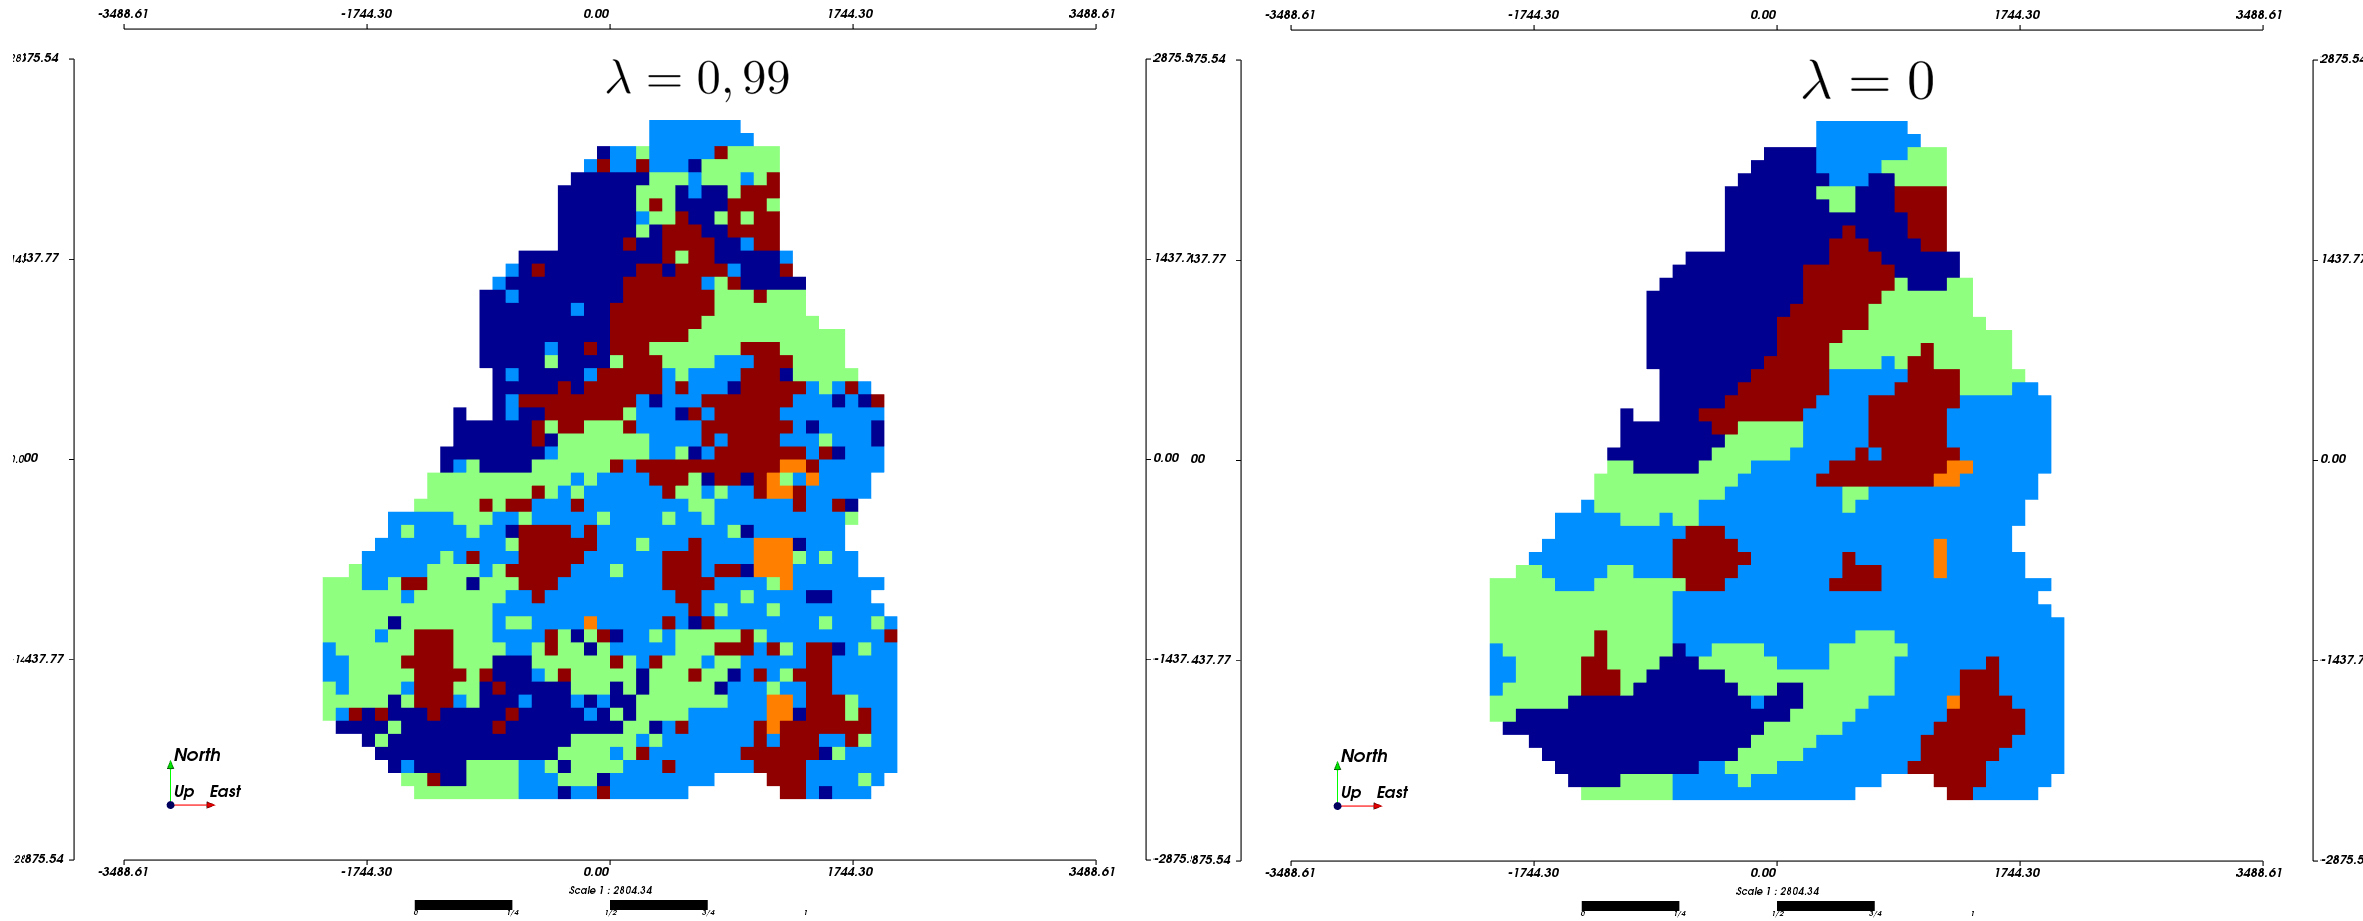
\includegraphics[width=0.6\textwidth]{modelagem_geologica/servosystem}
	\end{center}
	%\legend{Fonte: Modificado de \citeonline{maureira}}
\end{figure}

Alguns modelos podem apresentar efeito de borda, quando a influência de amostras localizadas nas bordas da malha de sondagem é extrapolada com exagero pelo algoritmo, criando estruturas inverossímeis. A aplicação do \textit{servo system} também controla a extensão desse tipo de estrutura, reduzindo o efeito de borda.

\section{O \textit{Plug-in}}

O método foi operacionalizado no \textit{software} geoestatístico de código aberto \textit{SGeMS}, com a criação de dois \textit{plug-ins} em linguagem \textit{python}. Os códigos podem ser encontrados no \autoref{apendicea} e \autoref{apendiceb}, bem como no repositório \textit{online} \url{https://github.com/LPM-UFRGS/dfmod}

No painel de algoritmos, há a opção \textit{DFMod} (\autoref{main_plugin}), que traz dois \textit{plugins}: \textit{signed distances} e \textit{interpolator}. O primeiro calcula o valor da função distância assinalada para cada amostra e para cada litologia. O segundo interpola a função distância, usando krigagem ordinária, para todo o \textit{grid}, além de apresentar opções de calcular a incerteza com \textit{softmax transformation} (\autoref{softmax_chap}) e corrigir as proporções com \textit{servo system} (\autoref{servo_chap}).

\begin{figure}[!ht]
	\caption{\label{main_plugin}Visão do painel de algoritmos do \textit{SGeMS} mostrando a opção \textit{DFMOD}.}
	\begin{center}
		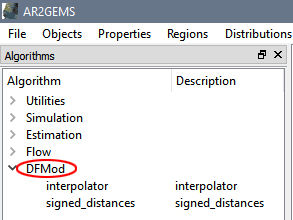
\includegraphics[width=0.5\textwidth]{modelagem_geologica/main}
	\end{center}
	%\legend{Fonte: Modificado de \citeonline{maureira}}
\end{figure}

\subsection{\textit{Signed distances}}\label{plugin_sg}

O \textit{plugin signed distances} (\autoref{sg_plugin}) calcula, para uma propriedade categórica, o valor da função distância anisotrópica (ou isotrópica), para cada amostra e cada litologia. O \textit{SGeMS} aceita apenas litologias codificadas em caracteres numéricos.   

\begin{figure}[H]
	\caption{\label{sg_plugin}Visão do \textit{plugin signed distances}.}
	\begin{center}
		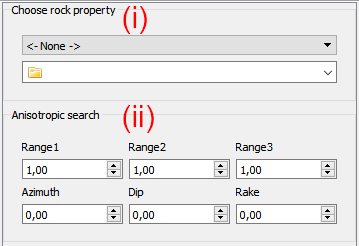
\includegraphics[width=0.5\textwidth]{modelagem_geologica/sg_plugin}
	\end{center}
	%\legend{Fonte: Modificado de \citeonline{maureira}}
\end{figure}

Em (i), usuário deve imputar a propriedade que informa a litologia (\textit{rock type}) de cada amostra. Em (ii), o usuário imputa os ângulos de rotação e razões de anisotropia, para o cálculo das distâncias anisotrópicas, o valor padrão calcula distâncias isotrópicas.

Como \textit{output}, o plugin gera uma propriedade \textit{signed distances RTX} para cada litologia, onde $X$ é o algarismo que representa aquela litologia.

O quadro Algoritmo 1 abaixo, mostra o funcionamento do algoritmo.

\begin{algorithm}[!ht]
\KwIn{Banco de dados categórico, ângulos de rotação e razões de anisotropia}
\KwOut{Propriedades \textit{signed distances RTX}}
Cria a matriz de rotação - dilatação/compressão\;
Transforma os dados originais $x,y,z$ em $x'',y'',z''$ com a matriz criada\;
Codifica as amostras, para cada domínio $k$, em $i_k(u_\alpha)$\; 
\For{litologias}{
	\For{amostras}{Calcula a distância entre cada amostra e todas as demais que pertencem a um domínio oposto\;
    Retém a distância mínima para cada amostra em uma lista\;
    Assinala de acordo com o indicador
}
Cria uma uma propriedade para cada litologia, referente a lista de menores distâncias criada em cada amostra (\textit{signed distances RTX})
}
\caption{Signed distances}
\end{algorithm}
 
\subsection{\textit{Interpolator}}\label{interpolator_sec}

O \textit{plugin interpolator} apresenta três abas: \textit{general, variogram} e \textit{options}. Na primeira aba (\autoref{interpolator_plugin}), o usuário deve imputar em (i) a propriedade categórica, nesse caso, para que os blocos que coincidem com amostras sejam carimbados com a respectiva litologia. Em (ii), o \textit{grid} no qual as distâncias serão interpoladas. Em (iii), o usuário deve imputar todas as distância \textit{signed distances RTX} calculadas com o \textit{plugin signed distances} (\autoref{plugin_sg}). Em (iv), a estratégia de busca da krigagem originária deve ser informada, número máximo e mínimo de dados condicionantes e elipsoide de busca.

\begin{figure}[H]
	\caption{\label{interpolator_plugin}Visão da aba \textit{general} do \textit{plugin interpolator}.}
	\begin{center}
		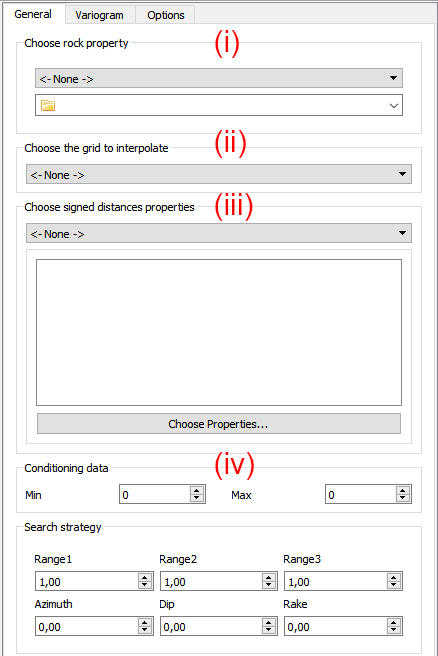
\includegraphics[width=0.5\textwidth]{modelagem_geologica/interpolator_plugin}
	\end{center}
	%\legend{Fonte: Modificado de \citeonline{maureira}}
\end{figure}

Na segunda aba (\autoref{variogram_plugin}), os modelos variográficos referentes a cada uma das propriedades \textit{signed distances RTX}, devem ser informados, na mesma ordem em que foram escolhidos na aba anterior (\autoref{interpolator_plugin} - (iii)). 

\begin{figure}[H]
	\caption{\label{variogram_plugin}Visão da aba \textit{variogram} do \textit{plugin interpolator}.}
	\begin{center}
		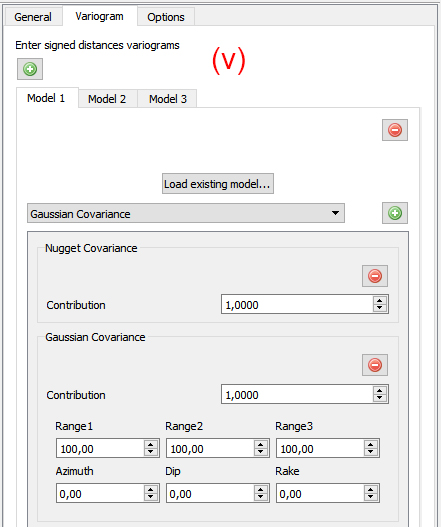
\includegraphics[width=0.5\textwidth]{modelagem_geologica/variogram_plugin}
	\end{center}
	%\legend{Fonte: Modificado de \citeonline{maureira}}
\end{figure}

Na terceira e última aba (\autoref{options_plugin}), o usuário escolhe se o modelo será pós processado. Em (vi), a opção \textit{softmax transformation} deve ser marcada, assim como o parâmetro $\gamma$ informado, em (vii), a opção \textit{servo system} deve ser marcada, o parâmetro $\lambda$ informado e a propriedade para a qual se deseja reproduzir as proporções imputada. A seleção do \textit{servo system} está condicionada à seleção da \textit{softmax transformation}. 

\begin{figure}[!ht]
	\caption{\label{options_plugin}Visão da aba \textit{options} do \textit{plugin interpolator}.}
	\begin{center}
		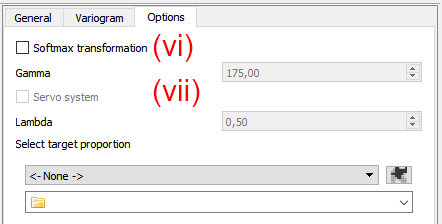
\includegraphics[width=0.5\textwidth]{modelagem_geologica/options_plugin}
	\end{center}
	%\legend{Fonte: Modificado de \citeonline{maureira}}
\end{figure}

Como \textit{output}, o \textit{plugin} gera, caso nenhuma opção da aba \textit{options} tenha sido selecionada, uma propriedade com o nome \textit{geo\_model}. Esse é o modelo geológico baseado na menor distância estimada para cada bloco. Ao marcar a opção \textit{softmax transformation}, uma propriedade \textit{Probability RTX} é criada, para cada litologia, onde $X$ é o algarismo que representa aquela litologia. Caso a opção \textit{servo system} seja selecionada, as propriedades \textit{Geologic\_Model\_Servo\_System} e \textit{Geologic\_Model\_Corrected} são criadas. A primeira representa o modelo criado a partir das probabilidades atualizadas e a segunda representa esse modelo suavizado (a correção é aplicada aqui uma única vez).

O quadro Algoritmo 2 abaixo mostra o funcionamento do algoritmo.

\begin{algorithm}[!ht]
\KwIn{Banco de dados categórico, propriedades \textit{signed distances RTX}, estratégia de krigagem, modelos variográficos, proporção alvo e parâmetros}
\KwOut{Propriedades \textit{geo\_model}, \textit{Probability RTX}, \textit{Geologic\_Model\_Servo\_System} e \textit{Geologic\_Model\_Corrected}}
\For{cada propriedade \textit{signed distances RTX}}{
Chama a krigagem ordinária no \textit{SGeMS} com os parâmetros imputados pelo usuário e interpola as distâncias calculadas para cada nó do grid informado\;}
\For{cada nó do grid}{Carimba no nó a categoria referente à menor distância estimada}
Cria a propriedade \textit{geo\_model}, baseada na menor distância interpolada\;
\If{opção \textit{softmax transformation} marcada}{
\For{cada propriedade interpolada}{
	\For{cada nó do grid}{Tranforma cada distância interpolada em probabilidade daquele nó pertencer a uma das litologias

}Cria uma propriedade \textit{Probability RTX} para cada litologia}
}
\If{opção \textit{servo system} marcada}{
Gera caminho aleatório\;
\For{nó do grid em caminho aleatório}{
Atualiza a proporção corrente marginal de cada categoria\;
\For{cada propriedade \textit{Probability RTX}}{
Atualiza as probabilidades de cada nó pertencer a cada uma das litologias de acordo com a diferença entre a proporção alvo e a proporção corrente marginal
}}
Cria a propriedade \textit{Geologic\_Model\_Servo\_System}\;
Suaviza o modelo e cria a propriedade \textit{Geologic\_Model\_Corrected}
}
Carimba nos blocos a categoria correspondente ao dado colocado
\caption{Interpolator}
\end{algorithm}

\section{Validação}

Os \textit{plugins} desenvolvidos foram validados tendo como referência resultados análogos da rotina \textit{DFMod} da biblioteca de algoritmos geoestatísticos \textit{GSLib}. Foi utilizado um banco de dados em três dimensões que possui 3276 amostras de 5 categorias diferentes para a validação do cálculo da função distância e modelo gerado a partir das distâncias estimadas. Ainda foi utilizado o \textit{jura data set} \cite{goovaerts1997geostatistics} para validação da \textit{softmax transformation} e \textit{servo system}.

Distâncias anisotrópicas foram calculadas com os parâmetros da \autoref{valid_rot}, escolhidos de forma arbitrária. E os resultados comparados.

\begin{table}[!ht]
\centering
\caption{Ângulos de rotação e proporções entre as direções principais usadas no cálculo da função distância anisotrópica.}
\label{valid_rot}
\begin{tabular}{lccc}

Rotações   & 30º & 45º & 60º \\ \hline
Proporções & 2  & 5  & 9  \\ 
\end{tabular}
\end{table}

A \autoref{dist_valid} mostra os \textit{scatterplots} entre as distâncias calculadas com o \textit{plugin} desenvolvido, no eixo $y$, contra as calculadas a partir da rotina \textit{DFMod} do \textit{GSLib} no eixo $x$, para todas as cinco categorias do banco de dados. A correlação é perfeita (100\%) para todos os gráficos.

\begin{figure}[H]
	\caption{\label{dist_valid}\textit{Scatterplot} entre as distâncias calculadas pelo \textit{plugin} desenvolvido contra distâncias calculadas a partir da rotina \textit{DFMod} do \textit{GSLib}.}
	\begin{center}
		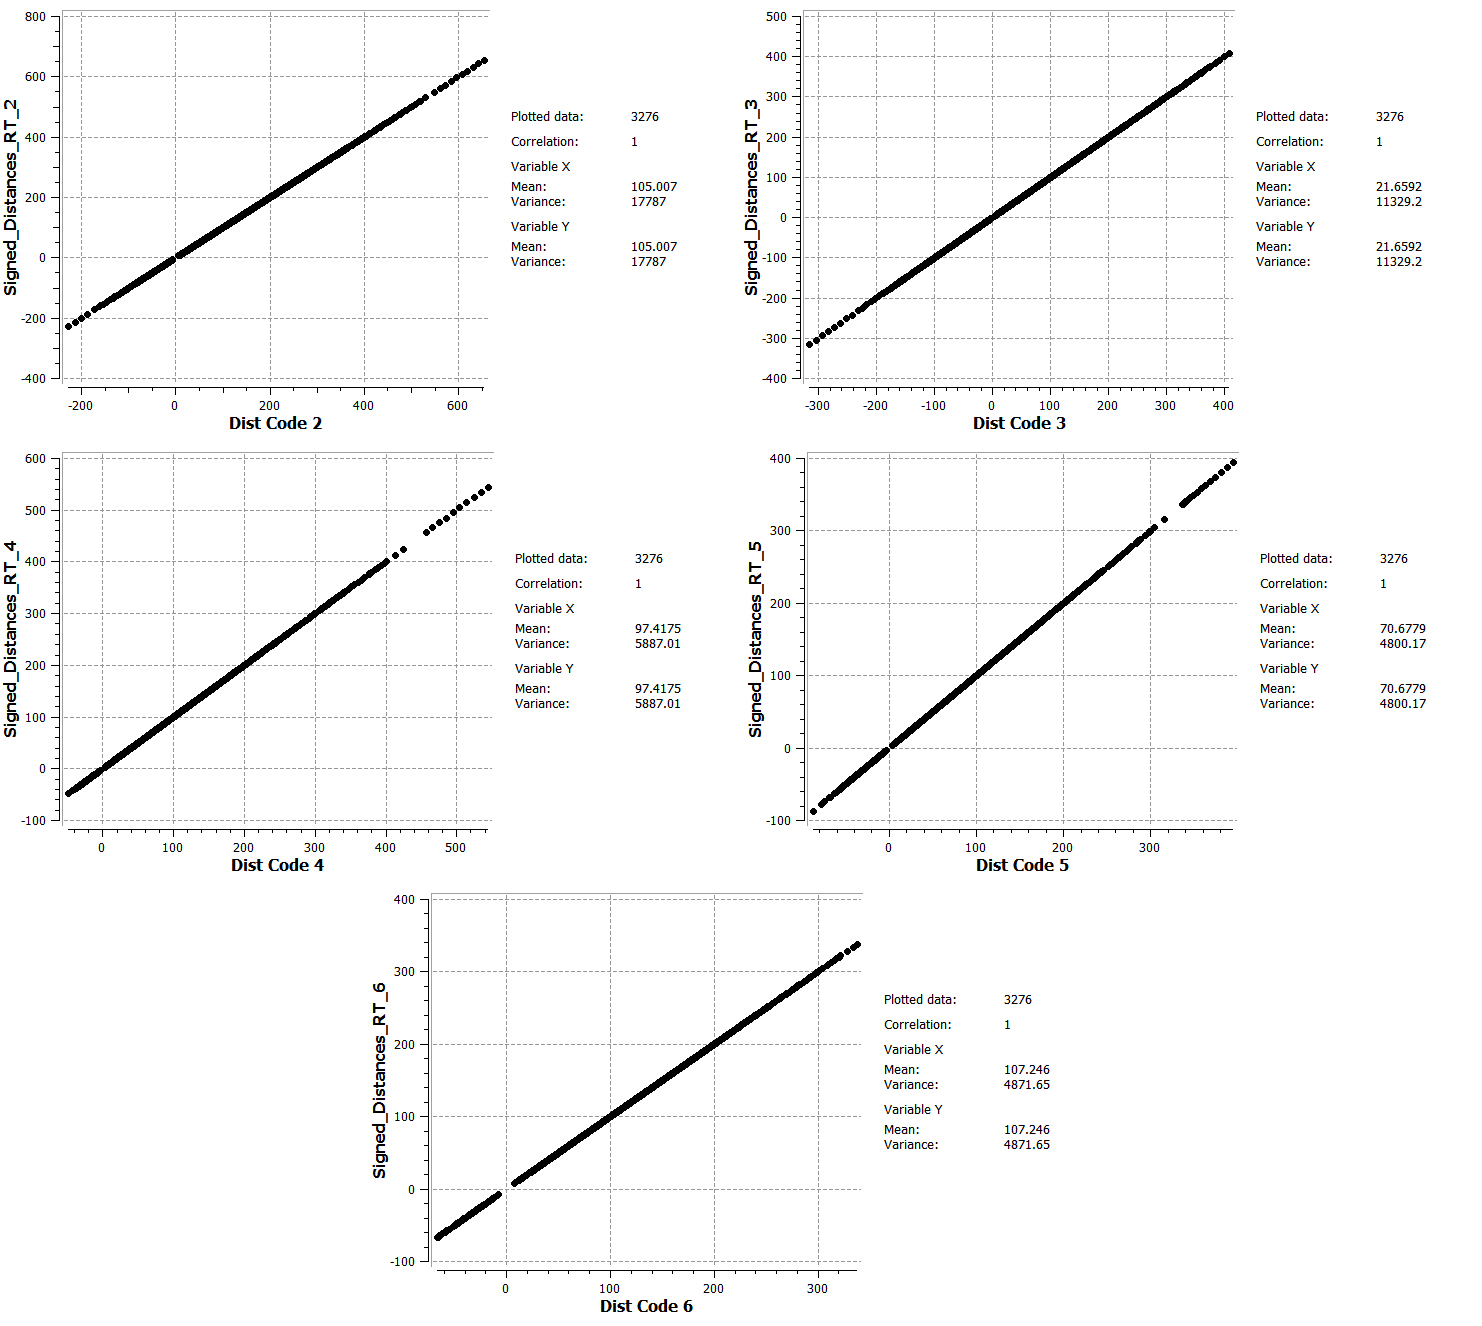
\includegraphics[width=0.8\textwidth]{modelagem_geologica/distances_valid}
	\end{center}
	%\legend{Fonte: Modificado de \citeonline{maureira}}
\end{figure}

Dois modelos foram gerados a partir dos  parâmetros do \autoref{anexo}. E foram comparados, novamente, em um \textit{scaterrplot} categórico (\autoref{model_valid}). O modelo gerado pelo \textit{plugin} desenvolvido aparece no eixo $y$, e no eixo $x$, o modelo criado a partir da rotina \textit{DFMod} do \textit{GSLib}. 99,998\% dos blocos são concordantes em ambos os modelos, blocos concordantes caem sobre a linha x=y e blocos discordantes fora dela, existem apenas três blocos discordantes entre os modelos gerados. 100\% de blocos concordantes não pôde ser atingido devido a diferença entre os códigos e linguagens de programação, as rotinas do \textit{GSLib} são escritas em \textit{fortran 90} enquanto o \textit{SGeMS} e seus \textit{plugins}, em \textit{C++} e \textit{python}, respectivamente.

\begin{figure}[H]
	\caption{\label{model_valid}\textit{Scatterplot} entre os modelos criados pelo \textit{plugin} desenvolvido e rotina \textit{DFMod} do \textit{GSLib}.}
	\begin{center}
		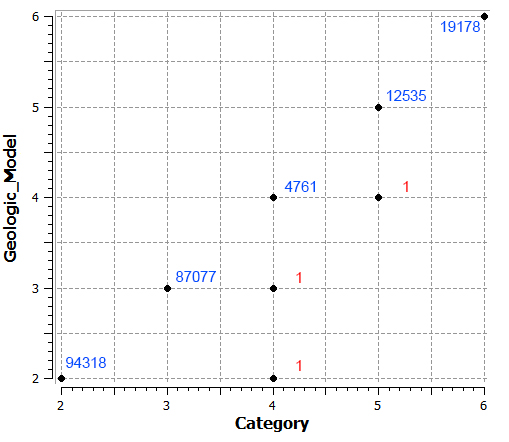
\includegraphics[width=0.8\textwidth]{modelagem_geologica/validation_models1}
	\end{center}
	%\legend{Fonte: Modificado de \citeonline{maureira}}
\end{figure}

Em nenhuma das versões do \textit{DFMod} encontradas nos repósitórios do \textit{GSLib} há versões funcionais, tanto da \textit{softmax transformation} quanto do \textit{servo system}. Então, como alternativa para validação, a correção \textit{servo system} foi executada no banco de dados jura, com um parâmetro $\lambda=0,99$. Dessa forma, é esperado que se, tanto o algoritmo da \textit{softmax transformation} quanto o algoritmo do \textit{servo system} (que depende do último), estejam corretos a proporção alvo seja reproduzida, ou pelo menos que um resultado bastante próximo seja obtido, já que não é possível usar um fator $\lambda=1$ (divisão por zero), que acarretaria na máxima correção possível, isto é, histogramas idênticos.

A \autoref{servo_valid} mostra os histogramas do modelo baseado somente nas distâncias estimadas à esquerda, dos dados ao centro (este foi utilizado como alvo para o \textit{servo system}), e do modelo após execução do \textit{servo system} à direita. As proporções alvo foram quase reproduzidas com perfeição, a diferença entre as médias dos histogramas é menor que 0,01.

\begin{figure}[H]
	\caption{\label{servo_valid}Histogramas do modelo baseado somente nas distâncias estimadas à esquerda, dos dados ao centro, e do modelo após execução do \textit{servo system} à direita.}
	\begin{center}
		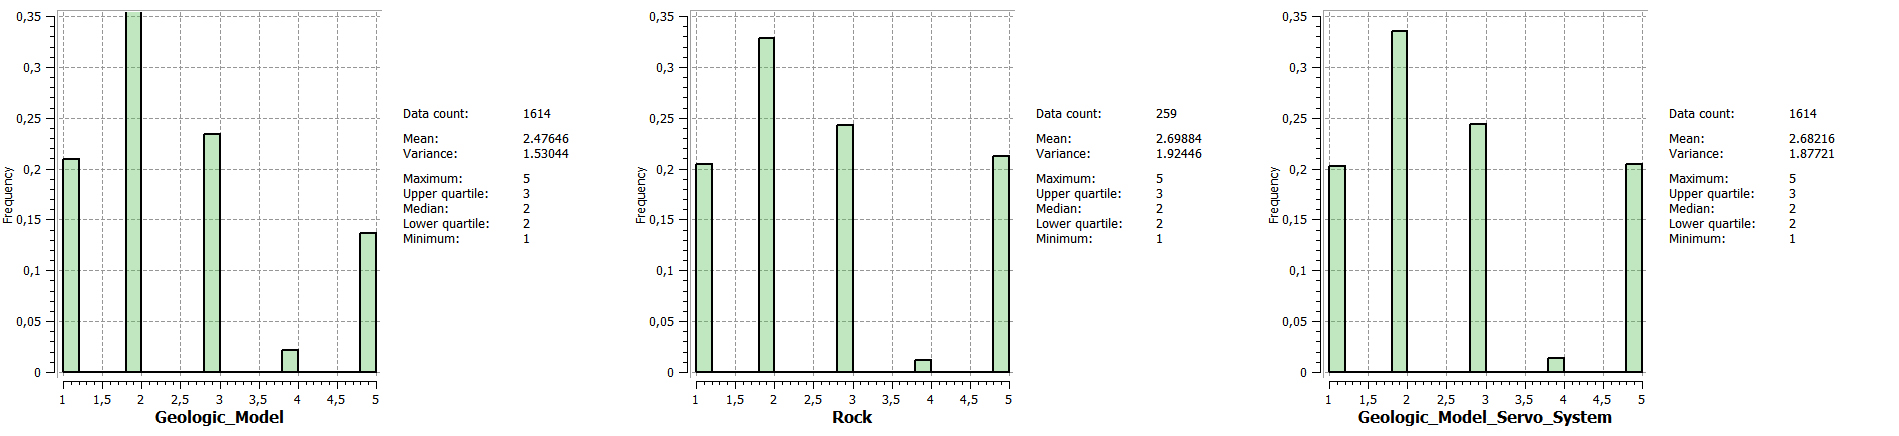
\includegraphics[width=\textwidth]{modelagem_geologica/servo_valid}
	\end{center}
	%\legend{Fonte: Modificado de \citeonline{maureira}}
\end{figure}
\chapter{Estudo de caso}\label{estudo_de_caso}

A metodologia desenvolvida no decorrer desse trabalho foi aplicada a um banco de dados real, proveniente de uma grande mineradora de ouro. Para verificar a competência do método, o modelo criado implicitamente pelo algoritmo proposto foi comparado com um modelo criado por um geomodelador, através da digitalização manual de polígonos em seções, e posterior construção dos sólidos que representam as unidades litológicas. Assim, foi possível avaliar se as estruturas geológicas interpretadas foram satisfatoriamente reproduzidas pelo algoritmo.

O banco de dados categóricos fornecido abrange 9140 amostras, distribuídas entre cinco diferentes litologias. O depósito cobre uma área de aproximadamente $10km^2$ com $1300m$ de profundidade. Maiores detalhes em relação à geologia e localização do depósito serão omitidos por questões de confidencialidade.

A \autoref{dados} evidencia as amostras em planta, à esquerda, e em perfil, à direita. Enquanto a \autoref{dados_hist}, mostra o histograma dos dados, que expressa as proporções de cada litologia nos dados amostrais.

\begin{figure}[H]
	\caption{\label{dados}Dados em planta à esquerda e em perfil à direita.}
	\begin{center}
		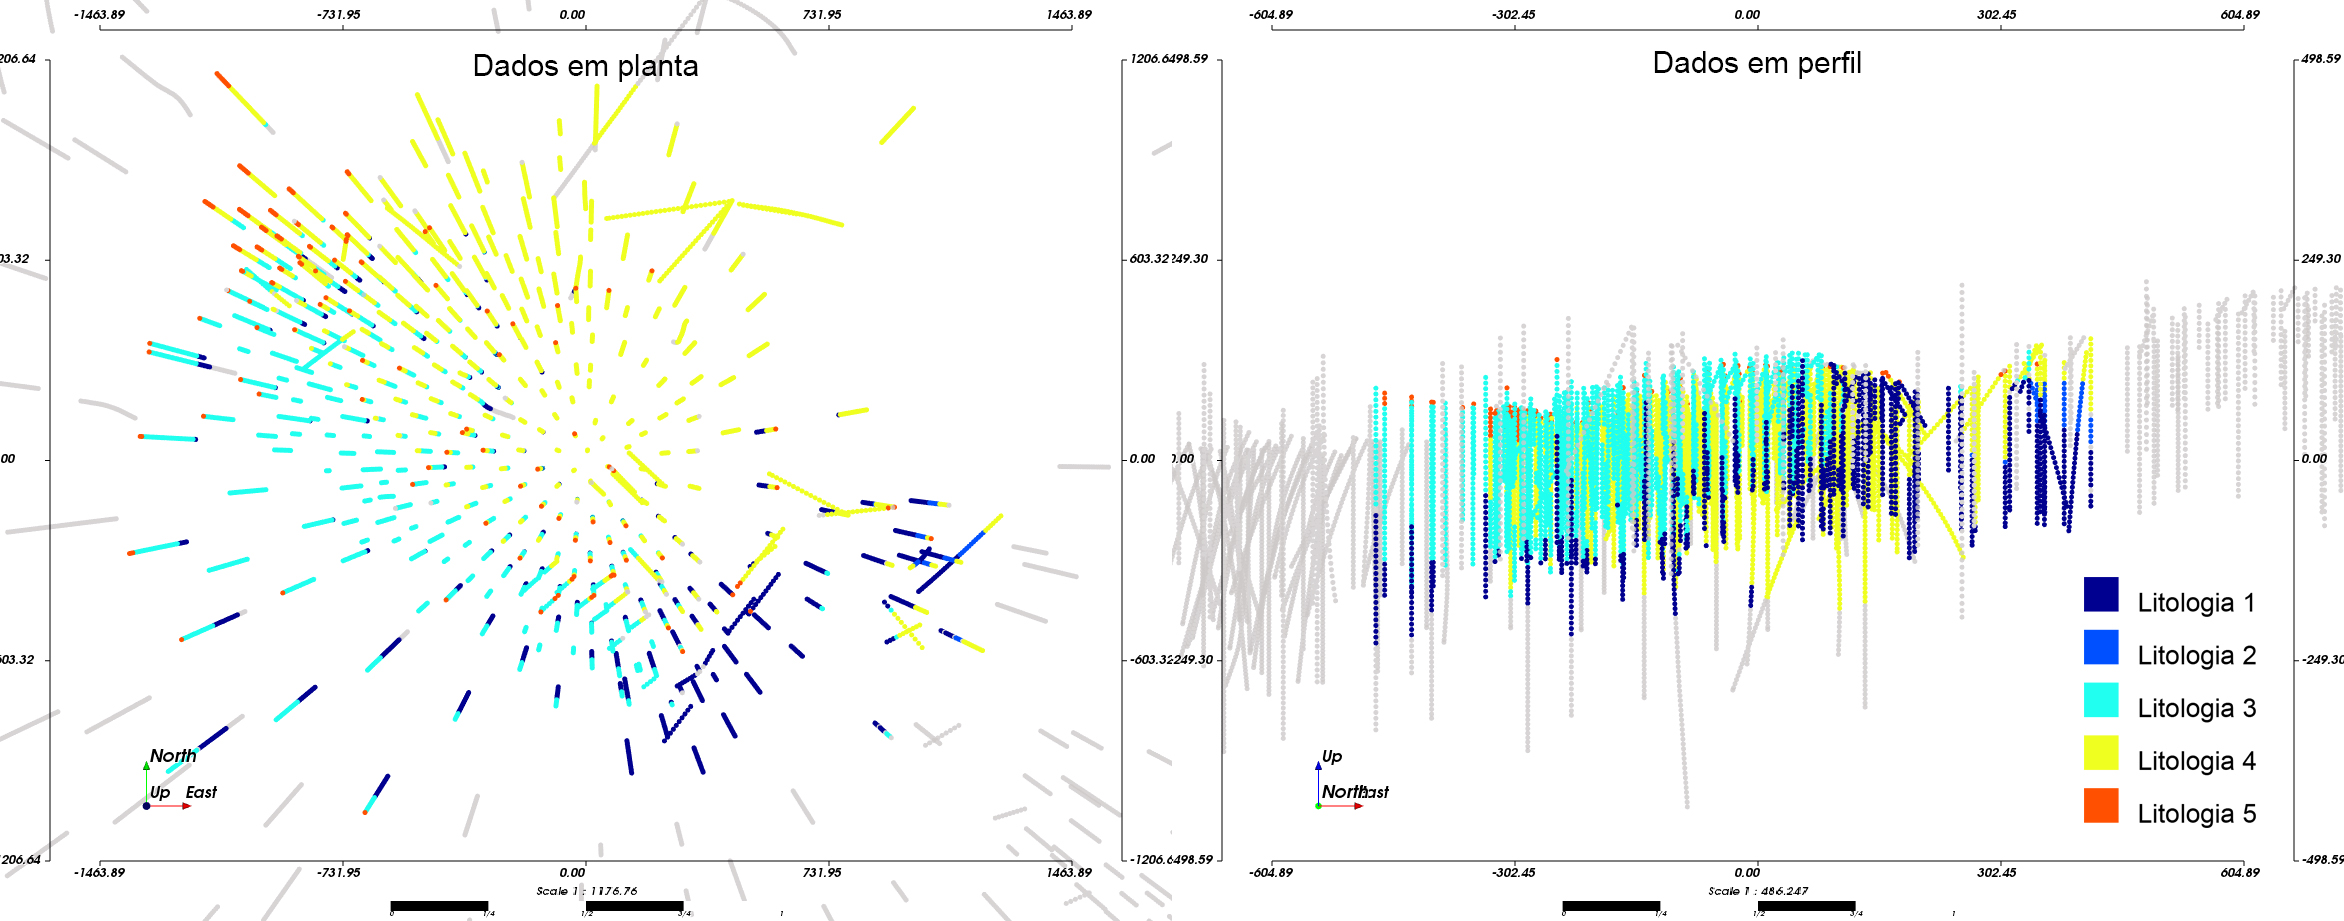
\includegraphics[width=\textwidth]{estudo_de_caso/dados}
	\end{center}
	%\legend{Fonte: Modificado de \citeonline{maureira}}
\end{figure}

\begin{figure}[!htb]
	\caption{\label{dados_hist}Histograma dos dados.}
	\begin{center}
		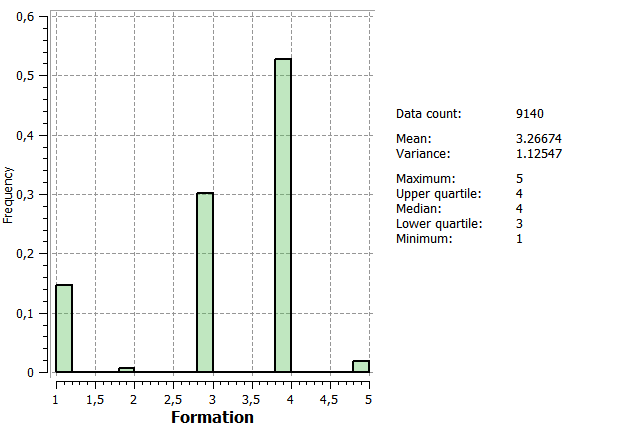
\includegraphics[width=0.5\textwidth]{estudo_de_caso/histograma_dados}
	\end{center}
	%\legend{Fonte: Modificado de \citeonline{maureira}}
\end{figure}

A partir das amostras, o valor da função distância assinalada foi calculado para cada litologia, em cada ponto amostral. O depósito não apresenta morfologia que justifique o cálculo de distâncias anisotrópicas, então, o caso isotrópico foi escolhido.

A \autoref{signed_distances_estudo} mostra as distâncias assinaladas calculadas para cada uma das cinco litologias, a transição suave entre as cores denota o comportamento extremamente contínuo das distâncias assinaladas.

\begin{figure}[H]
	\caption{\label{signed_distances_estudo}Distâncias assinaladas calculadas para cada uma das litologias.}
	\begin{center}
		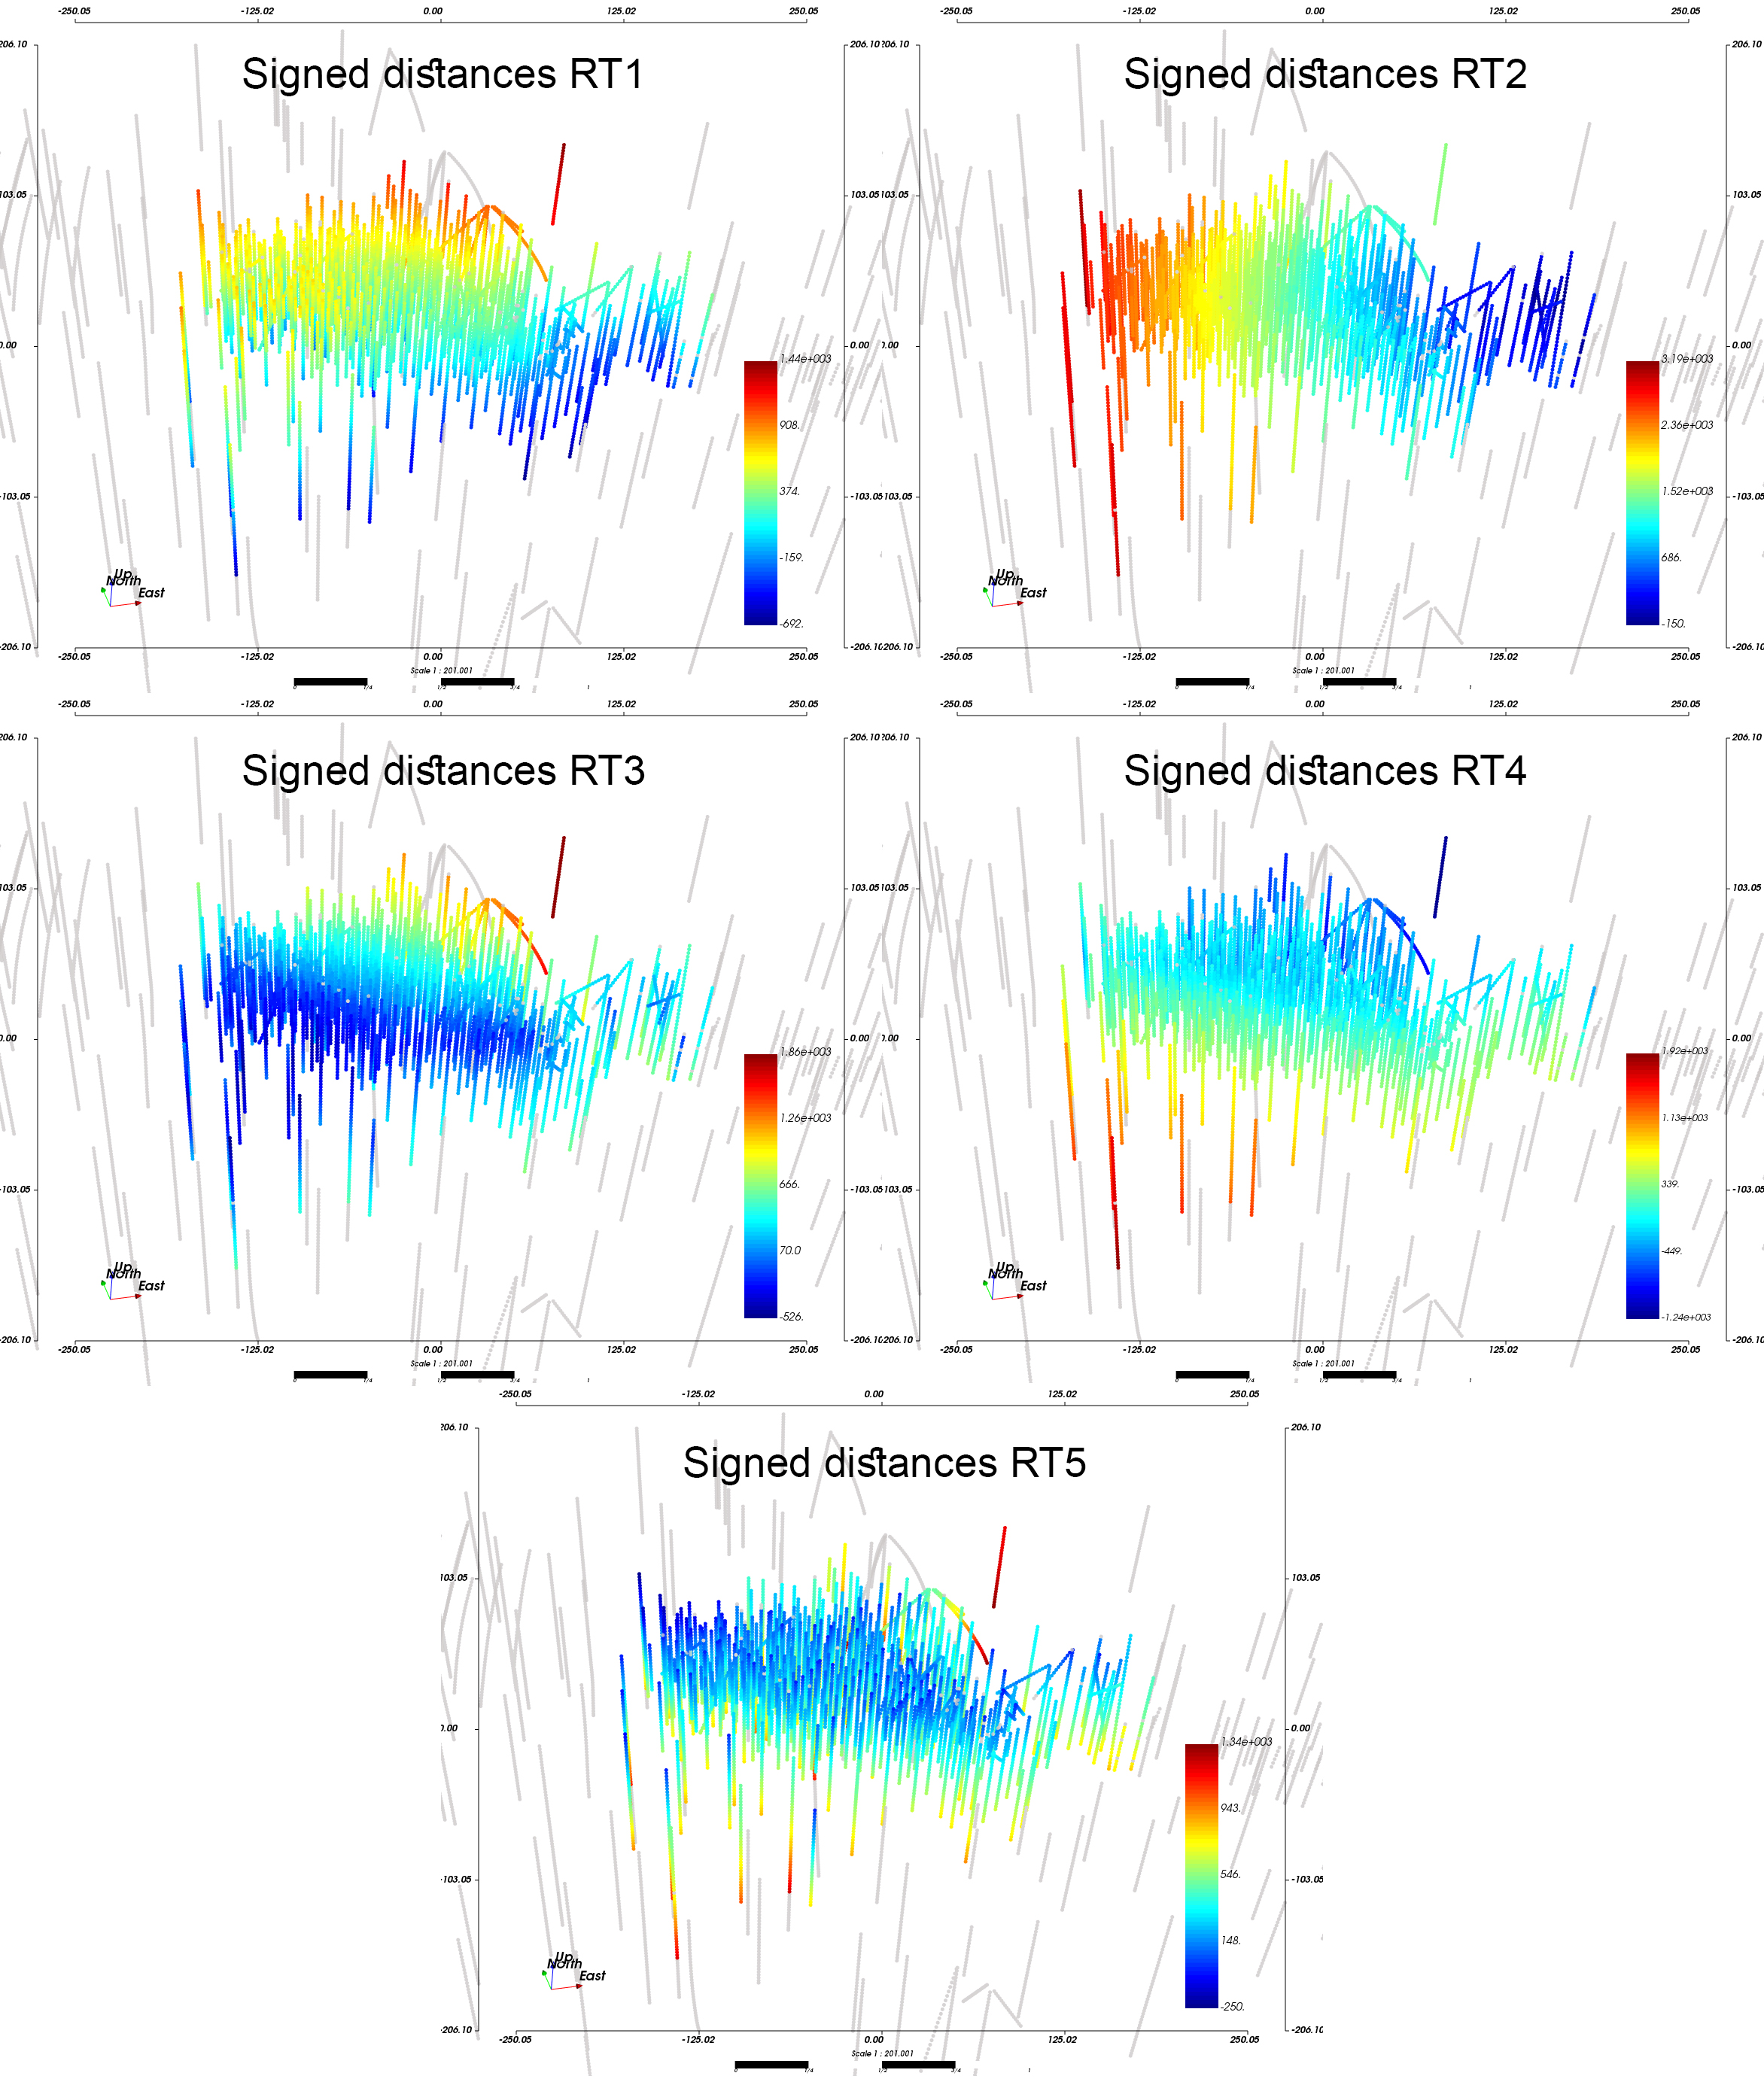
\includegraphics[width=0.9\textwidth]{estudo_de_caso/signed_distances}
	\end{center}
	%\legend{Fonte: Modificado de \citeonline{maureira}}
\end{figure}

\section{Variografia}

As distâncias assinaladas apresentam, além do comportamento extremamente contínuo observado na \autoref{signed_distances_estudo}, um comportamento não estacionário. Isto é, seu variograma experimental não se estabiliza em um patamar. Essa característica torna a inferência do alcance arbitrária, como observado na \autoref{variogramas}. 

O alcance do variograma, juntamente com a anisotropia, controlam a extensão e forma dos domínios modelados. Na \autoref{analise_range}, a litologia 1 foi modelada a partir de três valores diferentes de alcance de um variograma isotrópico, mantido o mesmo patamar: 150m à esquerda, 1500m no centro, e 15000m à direita. O variograma das demais litologias não foi alterado.

Ao aumentar o alcance do variograma de um dos domínios modelados, a estrutura associada à esse domínio ganha um corpo mais volumoso, crescendo na direção de maior continuidade do variograma, e consequentemente sua proporção no depósito aumenta, como observado na análise da litologia 1 da \autoref{analise_range}. A diferença entre as proporções não é muito pronunciada já que a densidade amostral do banco de dados é muito alta. Em análise semelhante, \citeonline{maureira} obteve resultados análogos.  

A inferência do alcance dos variogramas pode se tornar arbitrária devido ao comportamento não estacionário das distâncias assinaladas. Uma alternativa consiste em fixar a variância dos variogramas na variância \textit{a priori} dos dados, e ajustar um modelo ao variograma experimental dessa forma. Uma outra alternativa é inferir o alcance a partir das dimensões das estruturas observadas nos dados amostrais.

\begin{figure}[H]
	\caption{\label{analise_range}Litologia 1, e respectiva proporção, modelada variando o range do variograma: $150m$ à esquerda, $1500m$ ao centro e $15000m$ à direita.}
	\begin{center}
		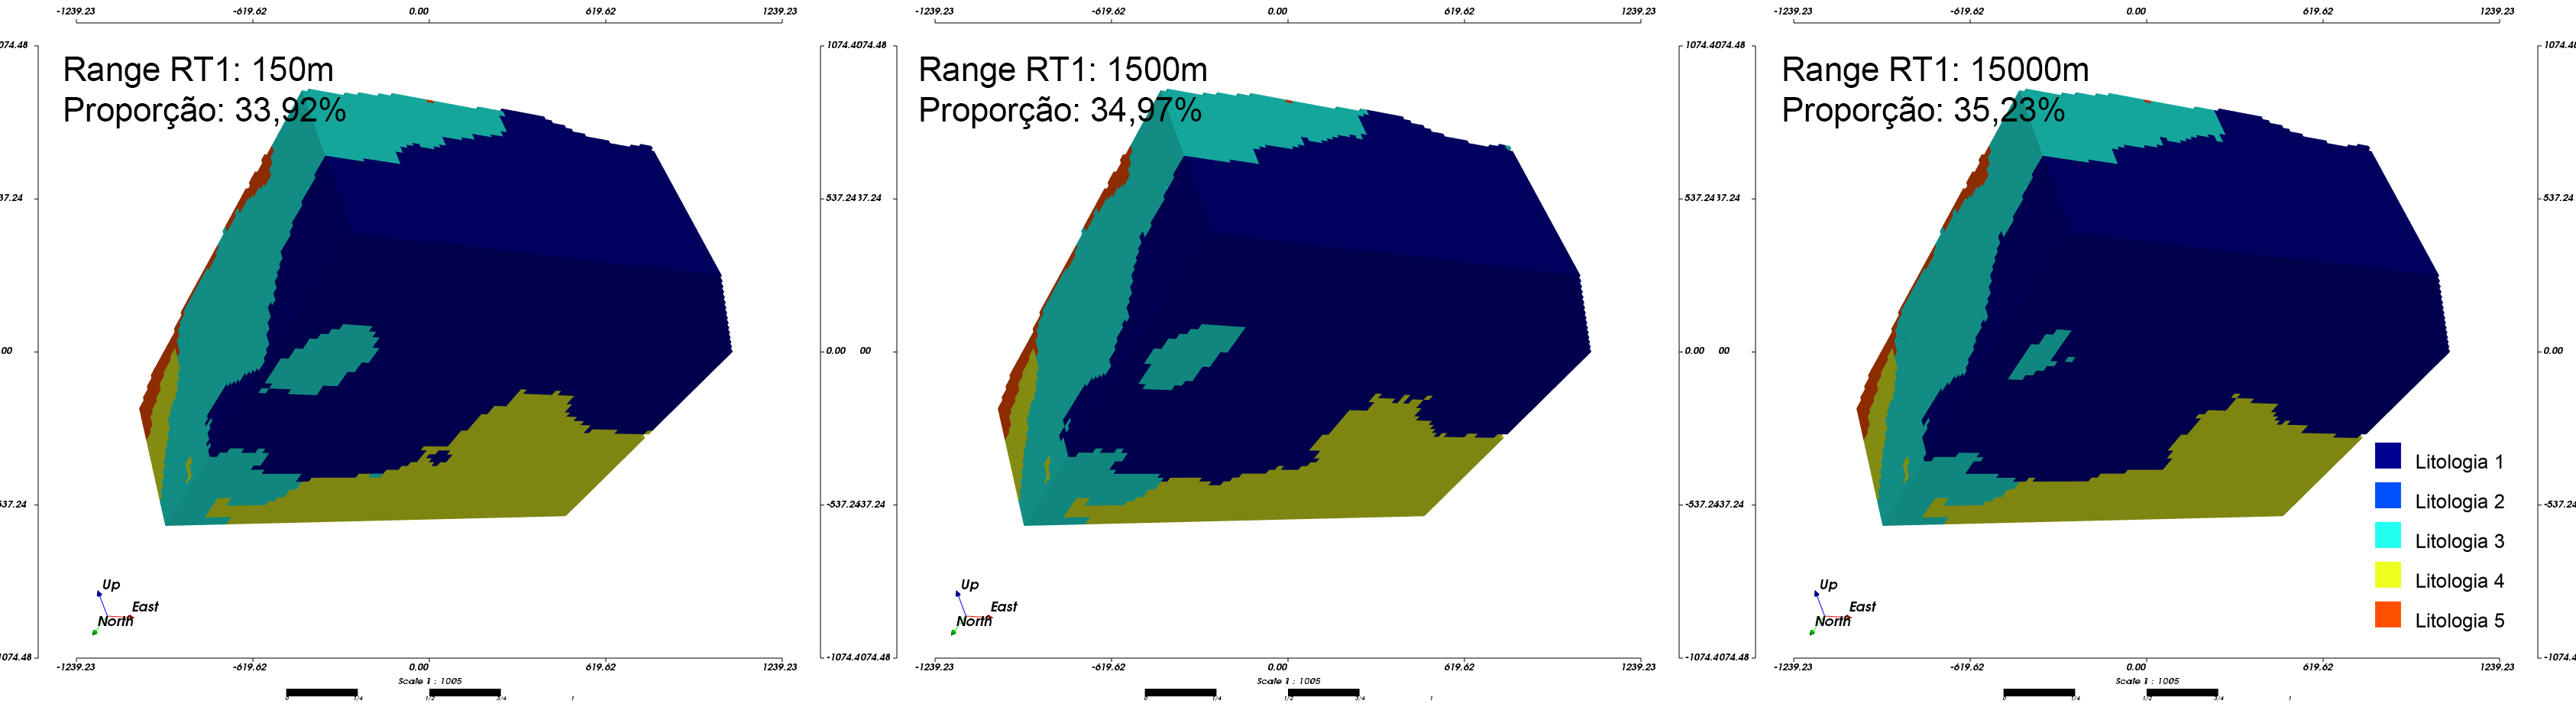
\includegraphics[width=\textwidth]{estudo_de_caso/analise_range}
	\end{center}
	%\legend{Fonte: Modificado de \citeonline{maureira}}
\end{figure}

Os variogramas experimentais das distâncias assinaladas nunca exibem efeito pepita. Porém, este pode ser adicionado arbitrariamente pelo usuário para controlar a interconectividade dos domínios. A \autoref{analise_efeito_pepita} mostra quatro modelos gerados a partir de variogramas isotrópicos com o mesmo alcance para todas as litologias e seus respectivos histogramas. Apenas a proporção entre a contribuição do efeito pepita e a contribuição total do variograma foi alterada, da mesma maneira, para todas as litologias.

Na \autoref{analise_efeito_pepita}, da esquerda para a direita, não há efeito pepita algum na primeira imagem, 10\% de efeito pepita na segunda imagem, 50\% e 90\% de efeito pepita nas imagens seguintes.

\begin{figure}[!htb]
	\caption{\label{analise_efeito_pepita}Modelos calculados a partir de variogramas com diferentes proporções de efeito pepita. Da direita para a esquerda: 0\%, 10\%, 50\% e 90\%.}
	\begin{center}
		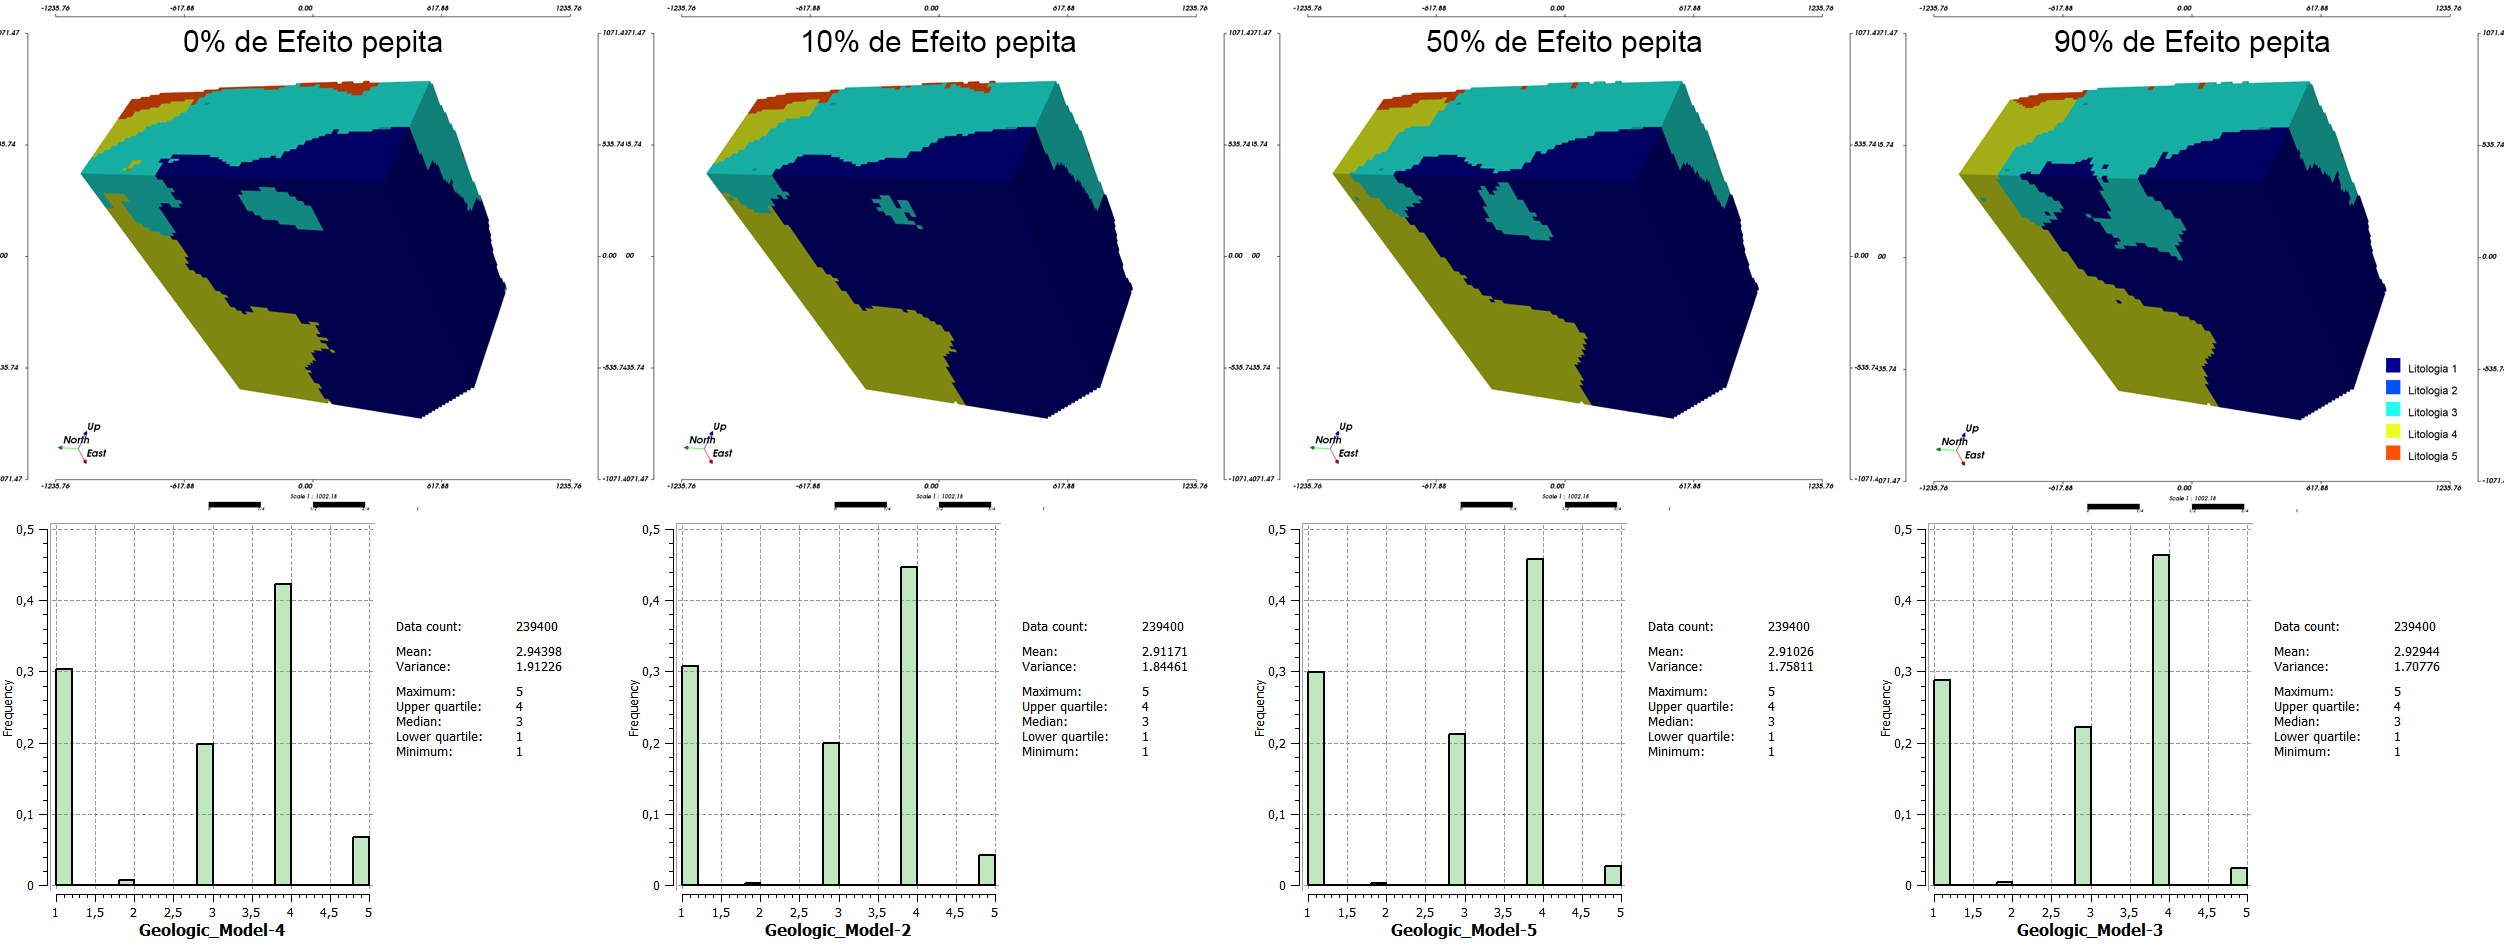
\includegraphics[width=\textwidth]{estudo_de_caso/efeito_pepita}
	\end{center}
	%\legend{Fonte: Modificado de \citeonline{maureira}}
\end{figure}

O efeito do aumento da contribuição do efeito pepita para a variância total é mais pronunciado na litologia 1, é possível observar que a medida que a contribuição aumenta o domínio representado pela litologia 1 se torna mais desconexo. Na última imagem (90\% de efeito pepita), pode-se observar dois "braços" que são interligados quando o modelo é gerado com proporções menores de efeito pepita nos variogramas. Os histogramas pouco se alteram, novamente, devido à alta densidade amostral do banco de dados.

Posto isso, os variogramas experimentais das distâncias assinaladas referentes às cinco litologias do depósito foram calculados, a partir dos parâmetros da \autoref{param_var}, e modelados. Os variogramas não apresentaram nenhuma direção preferencial de continuidade. A \autoref{variogramas} mostra os variogramas experimentais isotrópicos para todas as cinco distâncias assinaladas e seu respectivo modelo ajustado (\autoref{varsd1} a \autoref{varsd5}).

\begin{table}[!ht]
\centering
\caption{Parâmetros para o cálculo da variograma experimental.}
\label{param_var}
\begin{tabular}{cccc}
nº de lags & sep. lag (m) & tol. lag (m) & larg. de banda (m) \\ \hline
20         & 100      & 50       & 50             \\ \hline
\end{tabular}
\end{table}

O comportamento contínuo das distâncias faz com que o modelo gaussiano seja o que melhor se ajusta aos pontos do variograma experimental, geralmente, apenas uma estrutura é suficiente para um bom ajuste. O efeito pepita foi adicionado arbitrariamente para controlar a interconexão entre as litologias.

\begin{figure}[!htb]
	\caption{\label{variogramas} Variograma das distâncias assinaladas calculadas para cada uma das litologias.}
	\begin{center}
		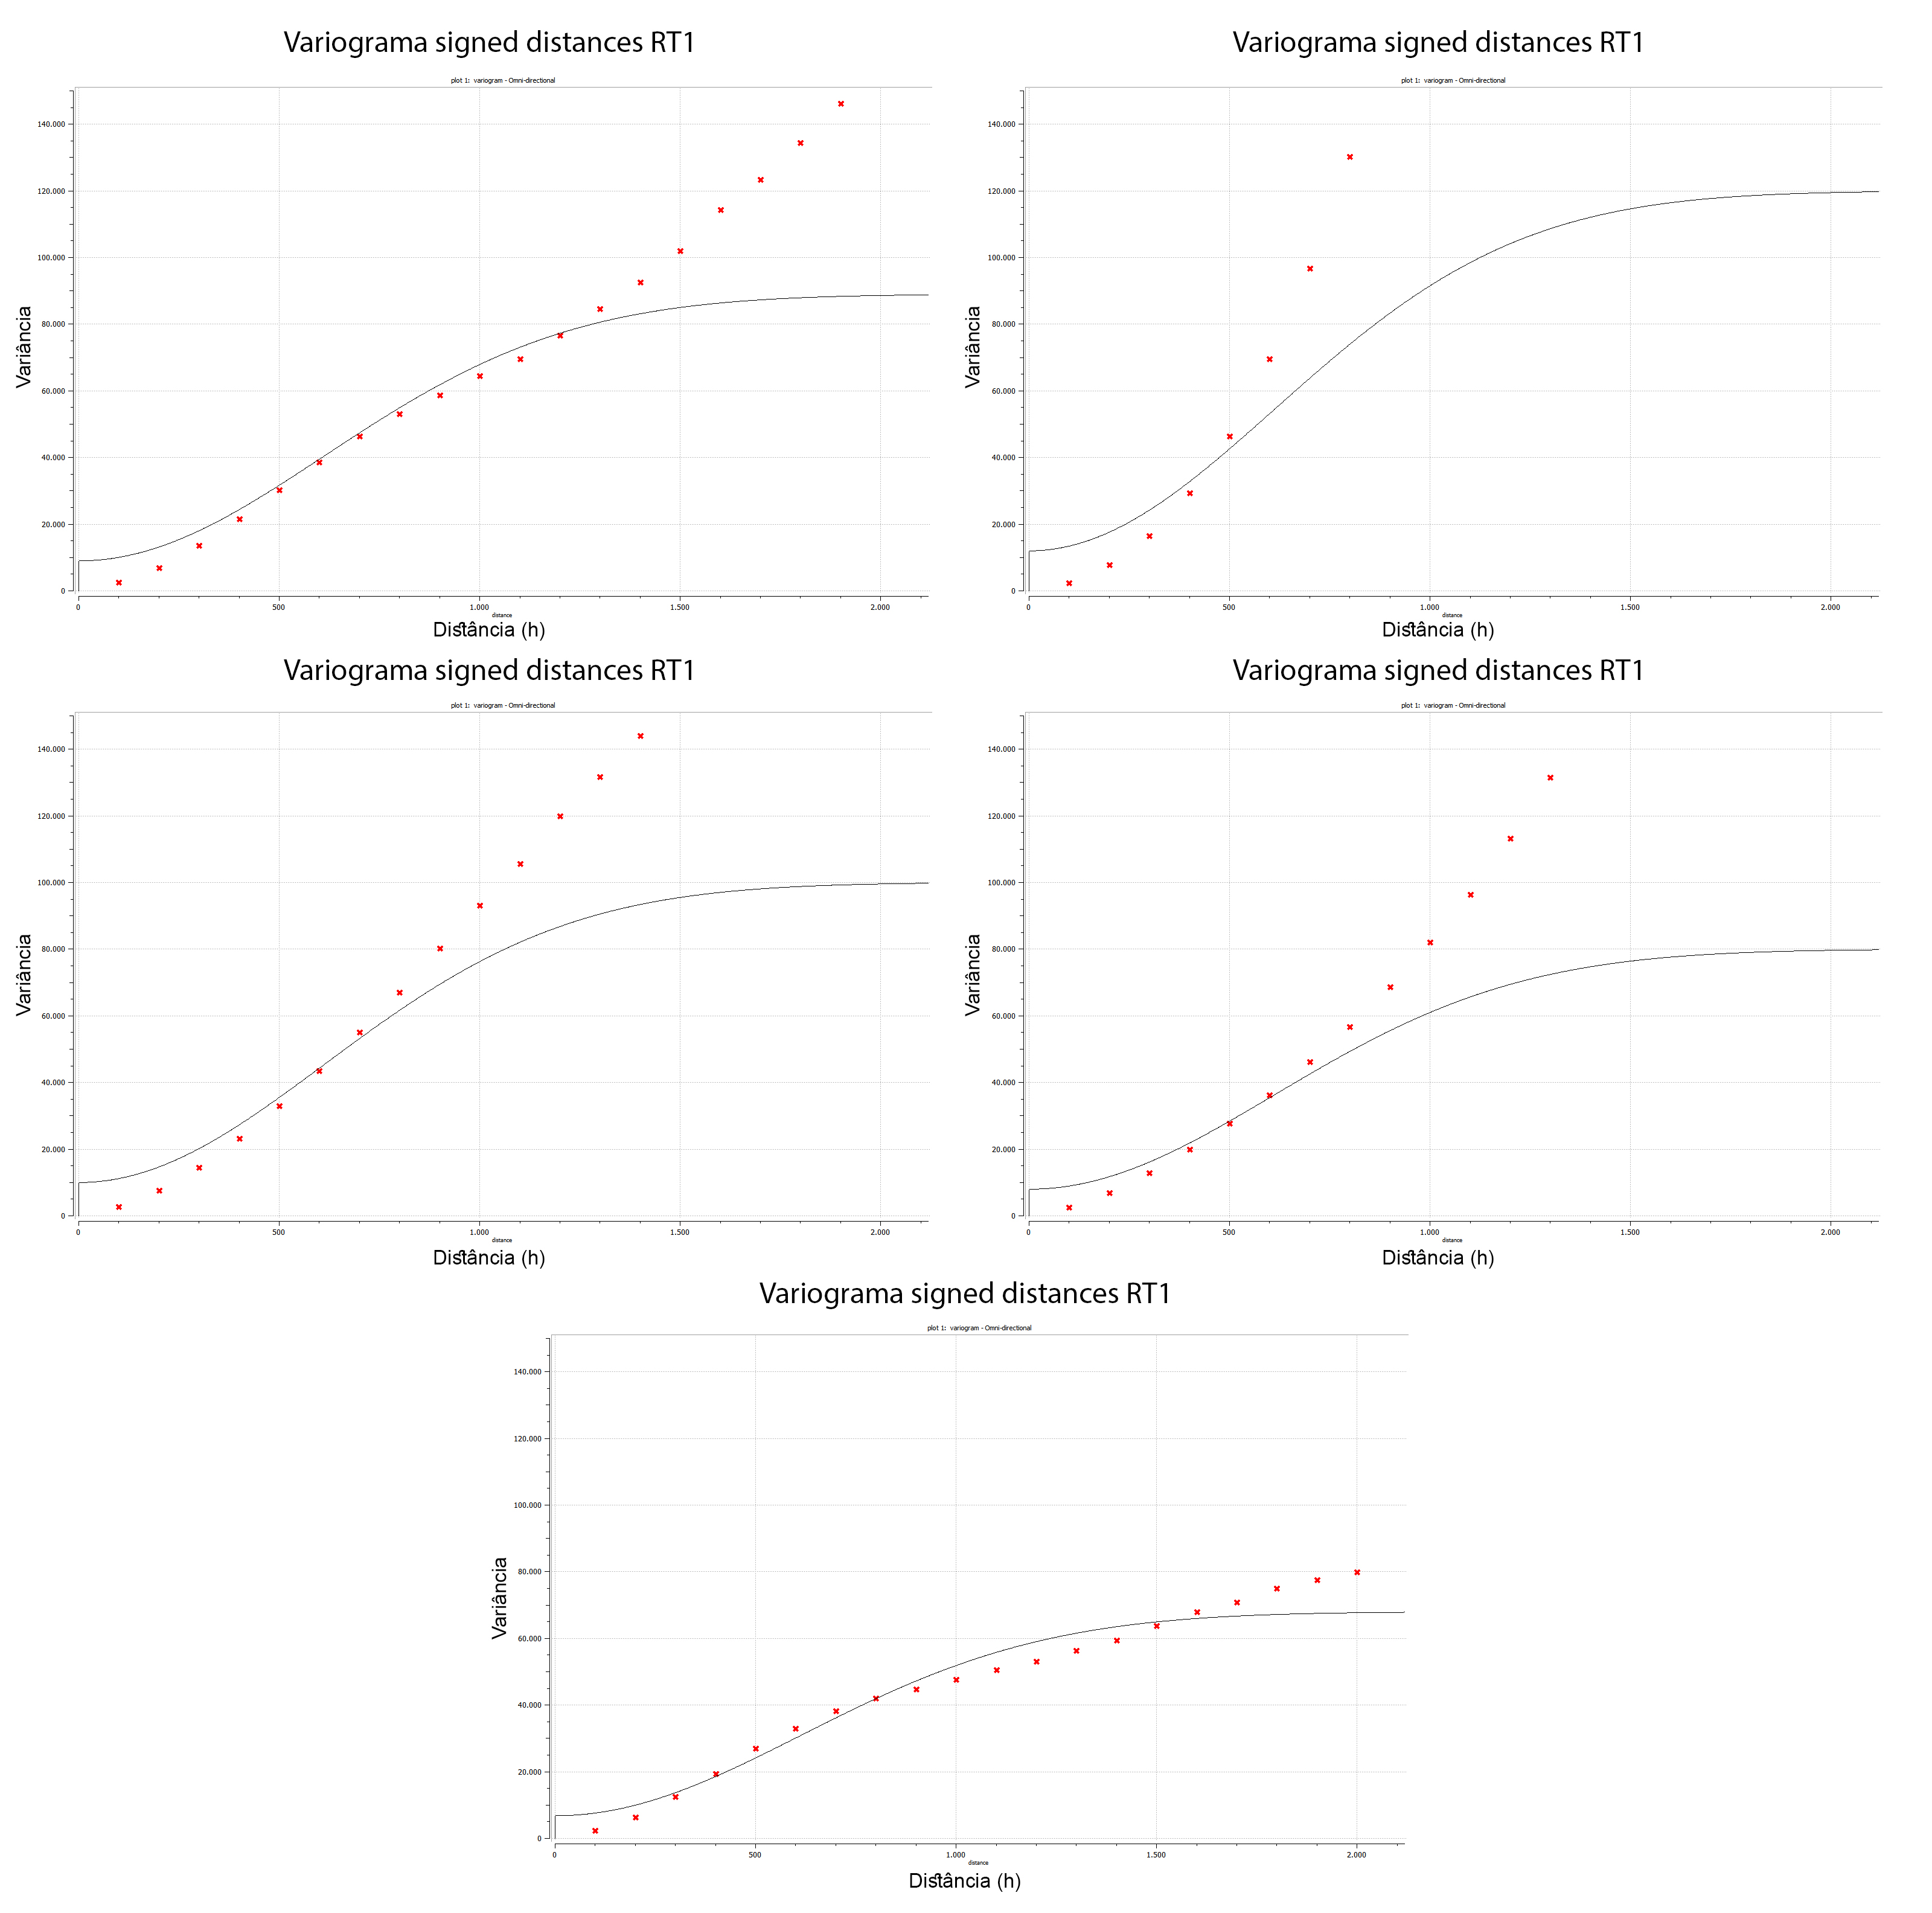
\includegraphics[width=\textwidth]{estudo_de_caso/var}
	\end{center}
	%\legend{Fonte: Modificado de \citeonline{maureira}}
\end{figure}

\begin{equation}
\label{varsd1}
\gamma_{SD1}(h)=9000+80000gauss\left(\frac{h}{1500m}\right)
\end{equation}

\begin{equation}
\label{varsd2}
\gamma_{SD2}(h)=12000+108000 gauss\left(\frac{h}{1500m}\right)
\end{equation}

\begin{equation}
\label{varsd3}
\gamma_{SD3}(h)=10000 +90000 gauss\left(\frac{h}{1500m}\right)
\end{equation}

\begin{equation}
\label{varsd4}
\gamma_{SD4}(h)=8000  +72000  gauss\left(\frac{h}{1500m}\right)
\end{equation}

\begin{equation}
\label{varsd5}
\gamma_{SD5}(h)=6800   +61200   gauss\left(\frac{h}{1500m}\right)
\end{equation}

O valor absoluto da variância dos variogramas não tem influência alguma no resultado da krigagem ordinária, somente na variância de krigagem, que não é usada para criar os modelos gerados implicitamente pelo método das distâncias assinaladas. Apenas a proporção das contribuições das estruturas para a variância total modifica o resultado da krigagem. Como os modelos ajustados aos variogramas experimentais da \autoref{variogramas} apresentam, todos eles, proporção de 10\% efeito pepita e 90\% de contribuição da estrutura gaussiana, além do mesmo range, foi possível o uso do mesmo modelo variográfico da \autoref{var} para todas as litologias.

\begin{equation}
\label{var}
\gamma_{SD}(h)=0,1+0,9gauss\left(\frac{h}{1500m}\right)
\end{equation}

\section{Interpolação}

As distâncias calculadas e posteriormente variografadas, foram interpoladas no mesmo \textit{grid} do modelo de referência fornecido. As propriedades do \textit{grid} são mostradas na \autoref{Grid_Parameters}. Uma máscara (\textit{region}) correspondente à topografia foi aplicada à esse \textit{grid}.  

\begin{table}[!htb]
\centering
\caption{Propriedades do \textit{grid}.}
\label{Grid_Parameters}
%\begin{adjustbox}{width=0.7\textwidth}
\begin{tabular}{cccccc}
\multicolumn{3}{c}{Número de blocos} & \multicolumn{3}{c}{Dimensão dos blocos (m)} \\ \hline
Num. X     & Num. Y     & Num. Z     & Dim. X     & Dim. Y     & Dim. Z     \\
70         & 60         & 57         & 50        & 50        & 25        \\ \hline
\end{tabular}
%\end{adjustbox}
\end{table}

As distâncias foram interpoladas por krigagem ordinária em todos os nós do \textit{grid}, com a estratégia de krigagem da \autoref{Kriging_parameter}.  

\begin{table}[!htb]
\centering
\caption{Parâmetros de krigagem ordinária.}
\label{Kriging_parameter}
%\begin{adjustbox}{width=0.7\textwidth}
\begin{tabular}{cccccc}
                & \multicolumn{3}{c}{Vizinhança de busca (m)}     & \multicolumn{2}{c}{Número de amostras} \\ \hline
                & Raio (X) & Raio (Y) & Raio (Z) & Min. amostras      & Max. amostras      \\
Litologias (1-5) & 3000      & 3000      & 3000      & 4                 & 40                \\ \hline
\end{tabular}
%\end{adjustbox}
\end{table}

A \autoref{num_amostras} mostra, à esquerda, um scatterplot categórico entre um modelo criado utilizando no máximo 40 amostras por estimativa, no eixo x, e no eixo y, um modelo criado usando no máximo 100 amostras por estimativa. E à direita, um outro \textit{scatterplot,} o mesmo modelo criado utilizando no máximo 40 amostras, no eixo x, e no eixo y, um modelo criado usando no máximo 200 amostras por estimativa. Todas as estratégias de krigagem utilizadas apresentam alcance de busca suficientemente grande para abranger o número máximo de amostras.

\begin{figure}[H]
	\caption{\label{num_amostras}Scatterplots entre modelos gerados com diferentes estratégias de krigagem.}
	\begin{center}
		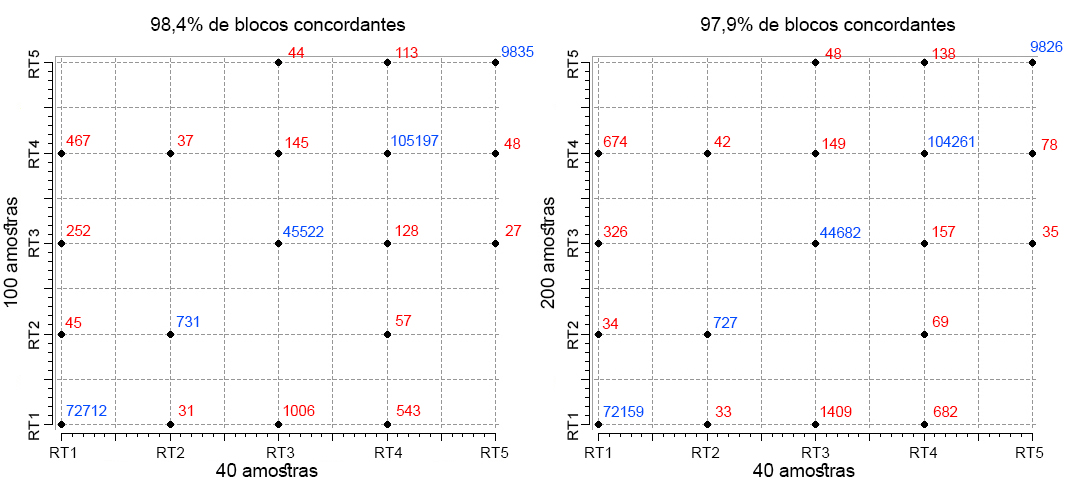
\includegraphics[width=\textwidth]{estudo_de_caso/num_amostras}
	\end{center}
	%\legend{Fonte: Modificado de \citeonline{maureira}}
\end{figure}

O modelo criado com 40 amostras e o modelo criado com 100 amostras apresentam 98,4\% dos blocos concordantes e o modelo criado com 40 amostras e 200 amostras 97,9\% dos blocos concordantes. No primeiro caso, a semelhança entre os modelos é suficientemente alta para justificar o uso de no máximo 40 amostras, tendo em vista que o tempo de execução do algoritmo passa de poucos minutos para algumas horas. No segundo caso, a diferença no número de blocos concordantes, para o primeiro caso, é extremamente baixa, e a diferença no tempo de execução significativa. O uso de mais do que 200 amostras por estimativa torna a aplicação do método, utilizando os \textit{plug-ins} em \textit{python} desenvolvidos, inviável. Isso se deve à uma limitação da própria linguagem de programação que trabalha apenas com um núcleo do processador por vez.

\section{Resultados}

Um modelo baseado na menor distância interpolada em cada bloco foi gerado pelo \textit{plug-in}, e é mostrado, em perspectiva, lado a lado com o modelo criado por um geomodelador na \autoref{modelo3d}. O modelo criado implicitamente pelo algoritmo à direita e o modelo criado, explicitamente, pelo geomodelador à esquerda. Cada litologia modelada foi colocada lado a lado separadamente para fins de comparação. 

\begin{figure}[H]
	\caption{\label{modelo3d}Comparação entre os modelos criados: modelo explícito à esquerda e modelo implícito à direita.}
	\begin{center}
		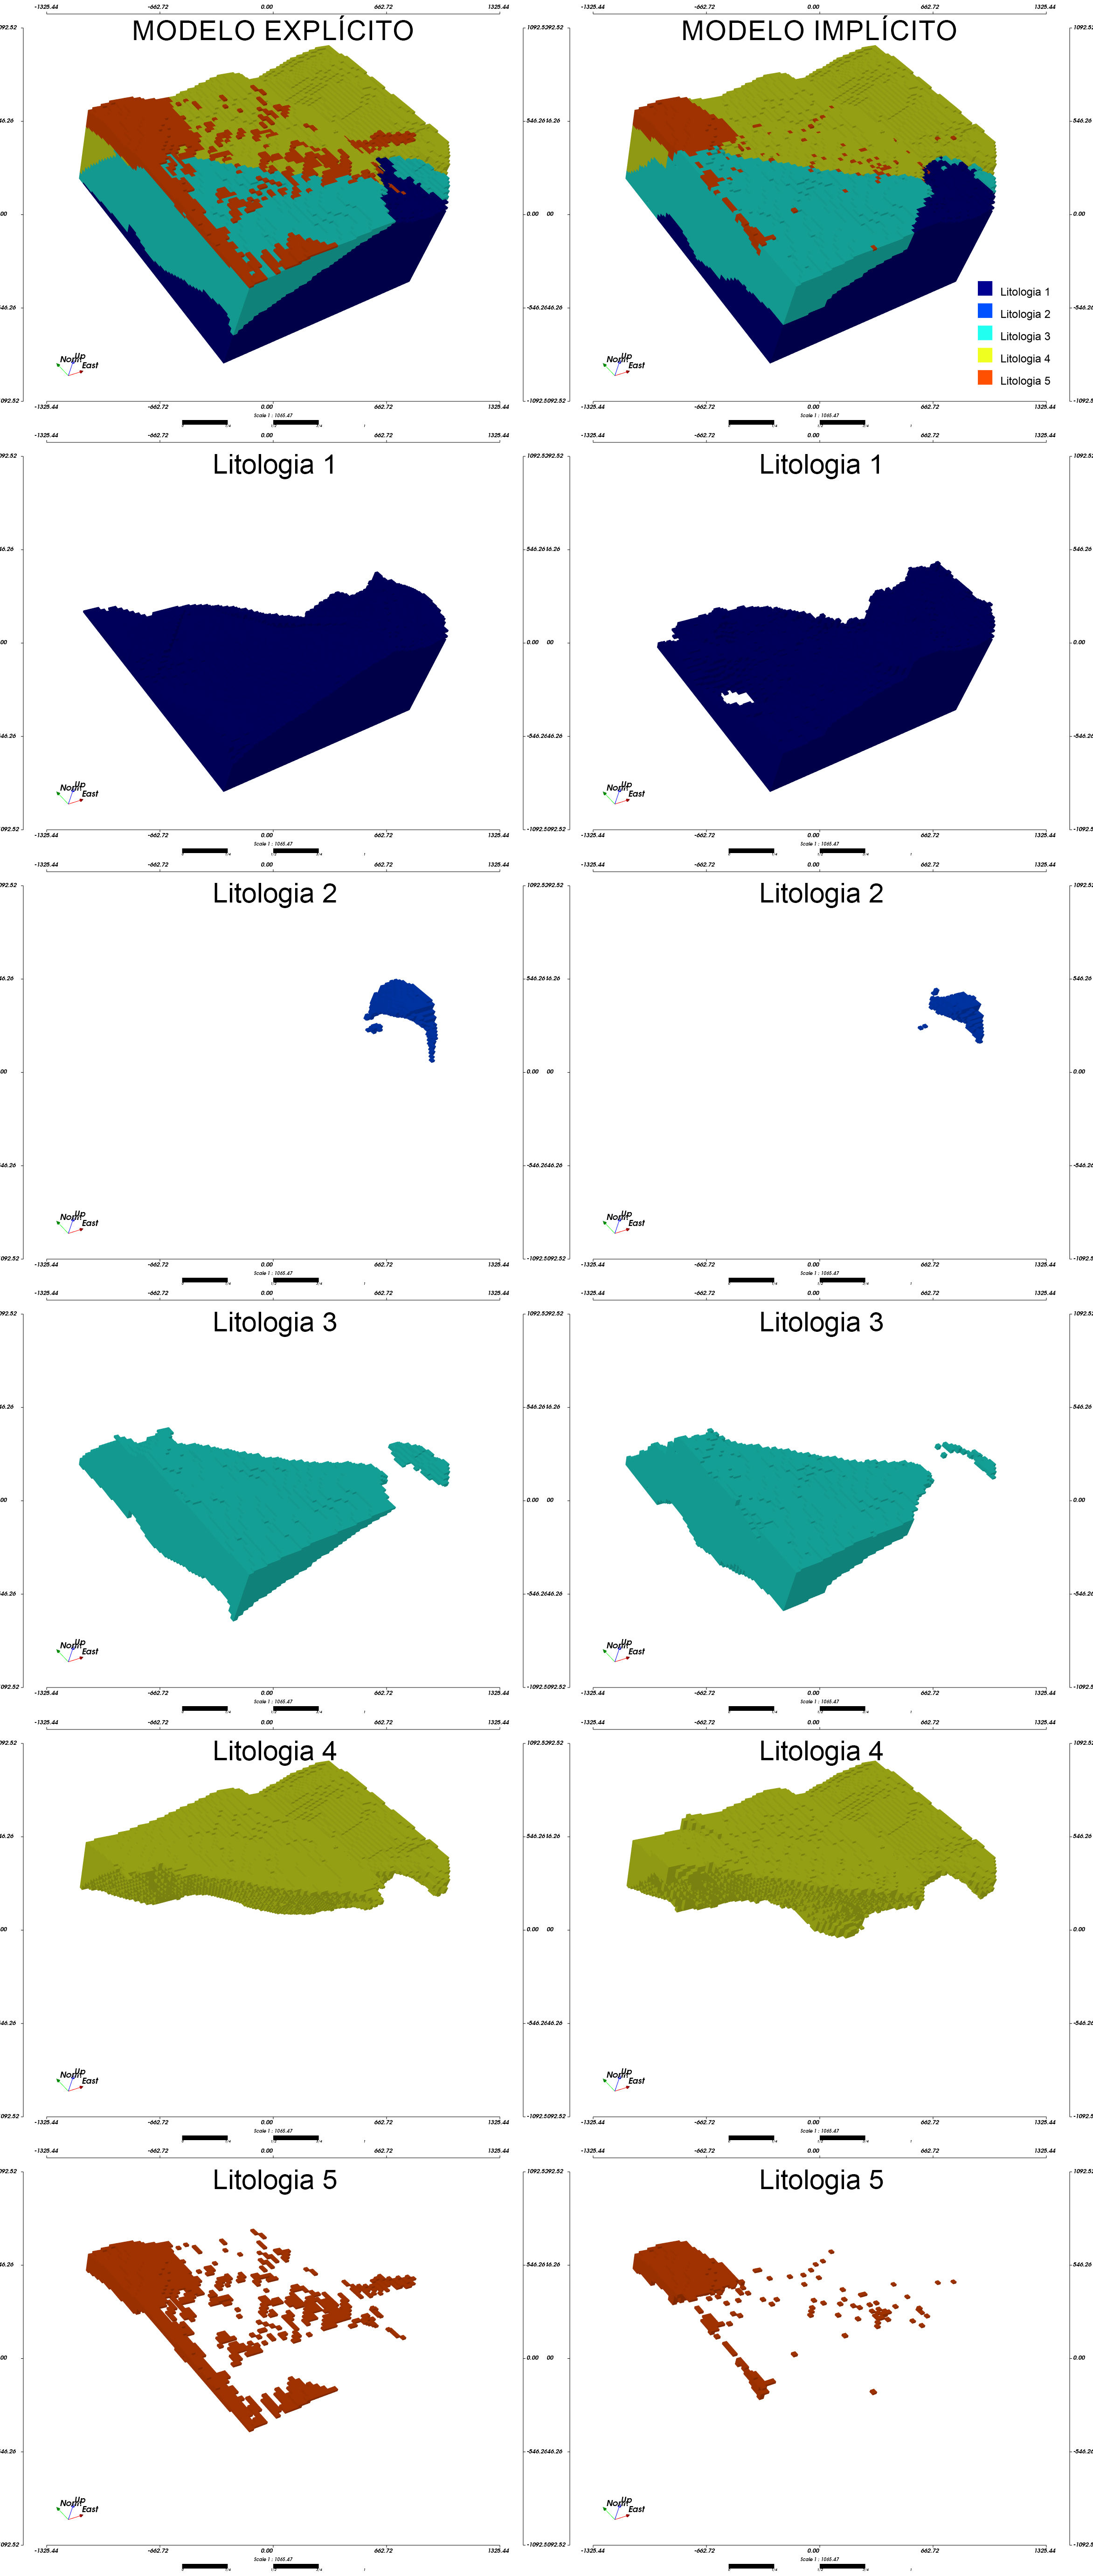
\includegraphics[width=0.65\textwidth]{estudo_de_caso/modelo3d}
	\end{center}
	%\legend{Fonte: Modificado de \citeonline{maureira}}
\end{figure}

A \autoref{scattermodelos} mostra o \textit{scatterplot} categórico entre os dois modelos criados: implícito no eixo y, e explícito no eixo x. Ao lado de cada ponto há o número de blocos comparados. Pontos que caem sobre a linha 45º são blocos concordantes em ambos os modelos, e pontos que caem fora dessa linha, blocos discordantes.

95\% dos blocos são concordantes em ambos os modelos. Todavia, apenas uma alta proporção de blocos concordantes não é indicativo de um bom modelo. Métodos menos sofisticados atingem alta proporção, 93\% no caso do vizinho mais próximo.   

\begin{figure}[H]
	\caption{\label{scattermodelos}\textit{Scatterplot} entre os modelos explícitos e implícitos.}
	\begin{center}
		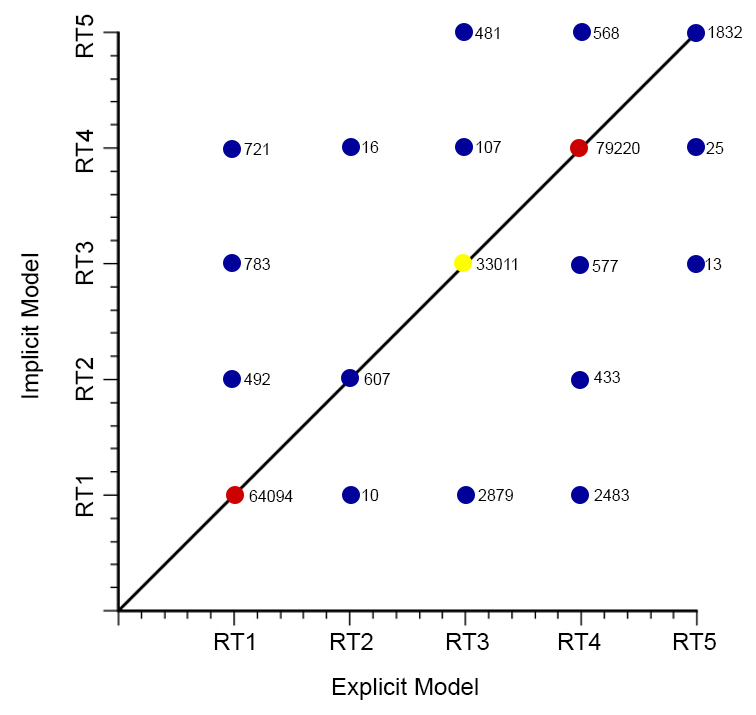
\includegraphics[width=0.7\textwidth]{estudo_de_caso/scatterplot_axis}
	\end{center}
	%\legend{Fonte: Modificado de \citeonline{maureira}}
\end{figure}

Porém, geram modelos que não fazem sentido físico do ponto de vista geológico, como observado na \autoref{nn}, um modelo gerado pela técnica do vizinho mais próximo a partir do mesmo banco de dados, são notáveis estruturas em forma de escada com mudança abrupta de angulação, diferentemente das formas suaves criadas pelo algoritmo proposto vistos na \autoref{modelo3d}.

\begin{figure}[H]
	\caption{\label{nn}Modelo criado utilizando a técnica do vizinho mais próximo.}
	\begin{center}
		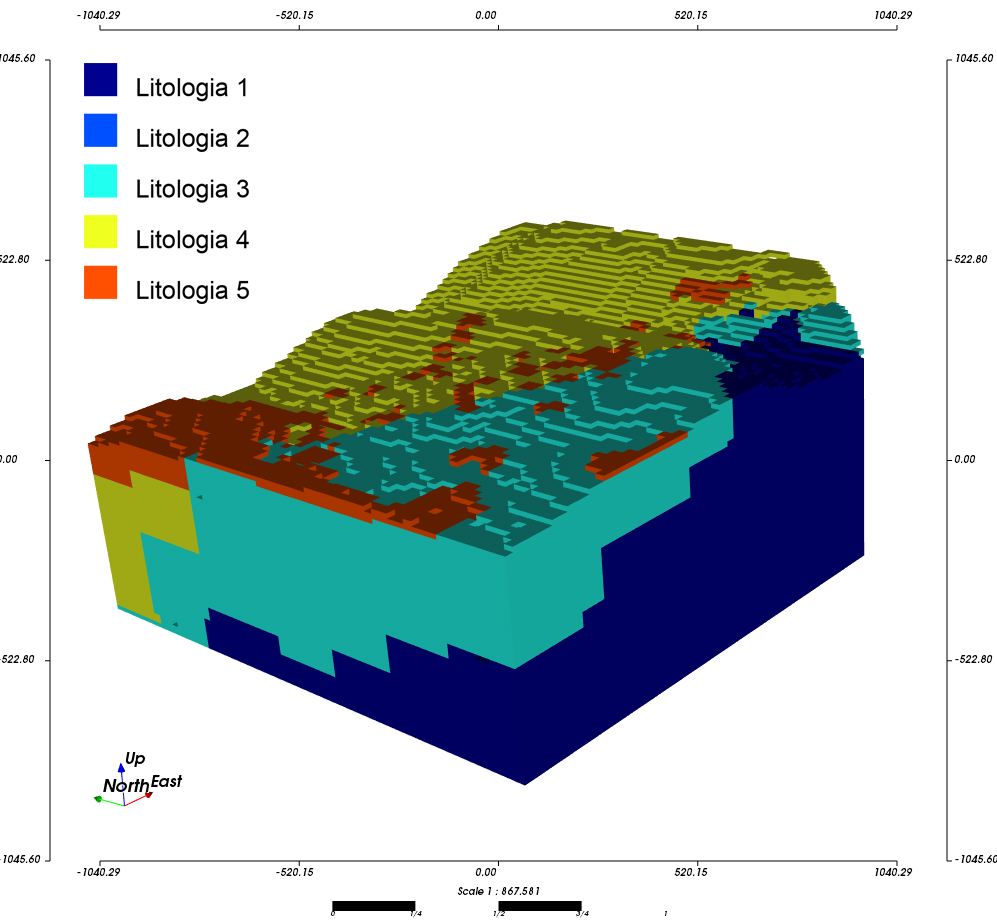
\includegraphics[width=0.6\textwidth]{estudo_de_caso/nn}
	\end{center}
	%\legend{Fonte: Modificado de \citeonline{maureira}}
\end{figure}

A incerteza também foi calculada como a probabilidade de cada de cada bloco pertencer a cada uma das categorias pela \textit{softmax transformation}. O parâmetro $\gamma=175$, valor padrão do \textit{plug-in}, foi escolhido. O resultado é mostrado nas seções verticais da \autoref{comparacao}.

\subsection{Comparação}\label{comparacao}

Uma comparação inicial pode ser feita observando os modelos, implícito e explícito, lado a lado na \autoref{modelo3d}. A litologia 5 aparece como blocos isolados e dispersos no modelo implícito, enquanto que no modelo explícito apresenta forma mais estruturada e contínua. Examinando a \autoref{dados}, percebe-se algumas amostras de litologia 5 espalhadas, em meio à abundantes amostras de outras litologias. O método das distâncias assinaladas não atribuirá aos blocos ao redor de amostras dispersas, sua litologia, já que a menor distância estimada para esses blocos será referente à categoria das amostras abundantes e agrupadas.

Os blocos isolados pertencentes à litologia 5 que aparecem no modelo implícito são blocos carimbados, após a geração do modelo baseado nas distâncias, com a litologia da amostra colocada, como visto no quadro Algoritmo 2 da \autoref{interpolator_sec}. O geomodelador aumentou a influência das amostras de litologia 5 no modelo explícito arbitrariamente ou munido de informação adicional, que não pode ser imputada no algoritmo proposto.

Para checar se o algoritmo reproduziu satisfatoriamente as estruturas interpretadas pelo geomodelador, seções verticais ao longo das direções x e y foram comparadas. Quatro seções espalhadas por toda extensão do modelo foram escolhidas em cada direção. 

Em x, o modelo apresenta 70 seções, a \autoref{secaox10} mostra a seção 10/70. À esquerda o modelo criado pelo geomodelador, ao centro o modelo criado pelo algoritmo proposto, à  direita blocos discordantes e concordantes e abaixo as probabilidades de cada bloco pertencer a cada uma das cinco categorias. Todas as seções analisadas seguem a mesma diagramação. 

Estruturas geológicas que foram reproduzidas satisfatoriamente pelo algoritmo foram destacadas por elipses verdes, enquanto estruturas que não foram bem reproduzidas, destacadas por elipses vermelhas.

Na região destacada pela elipse vermelha da \autoref{secaox10}, não há amostras da litologia 1. Provavelmente, o geomodelador munido de sua experiência e/ou informação adicional atribuiu a litologia 1 aos blocos dessa região. Note que alguns blocos na superfície do modelo implícito não foram carimbados com a litologia 5 como no modelo explícito. Porém, ao analisar a probabilidade RT5, existe uma chance considerável desses blocos pertencerem à litologia 5. mesmo que não tenham sido atribuídos àqueles blocos.   

\begin{figure}[H]
	\caption{\label{secaox10}Seção vertical 10/70 em x.}
	\begin{center}
		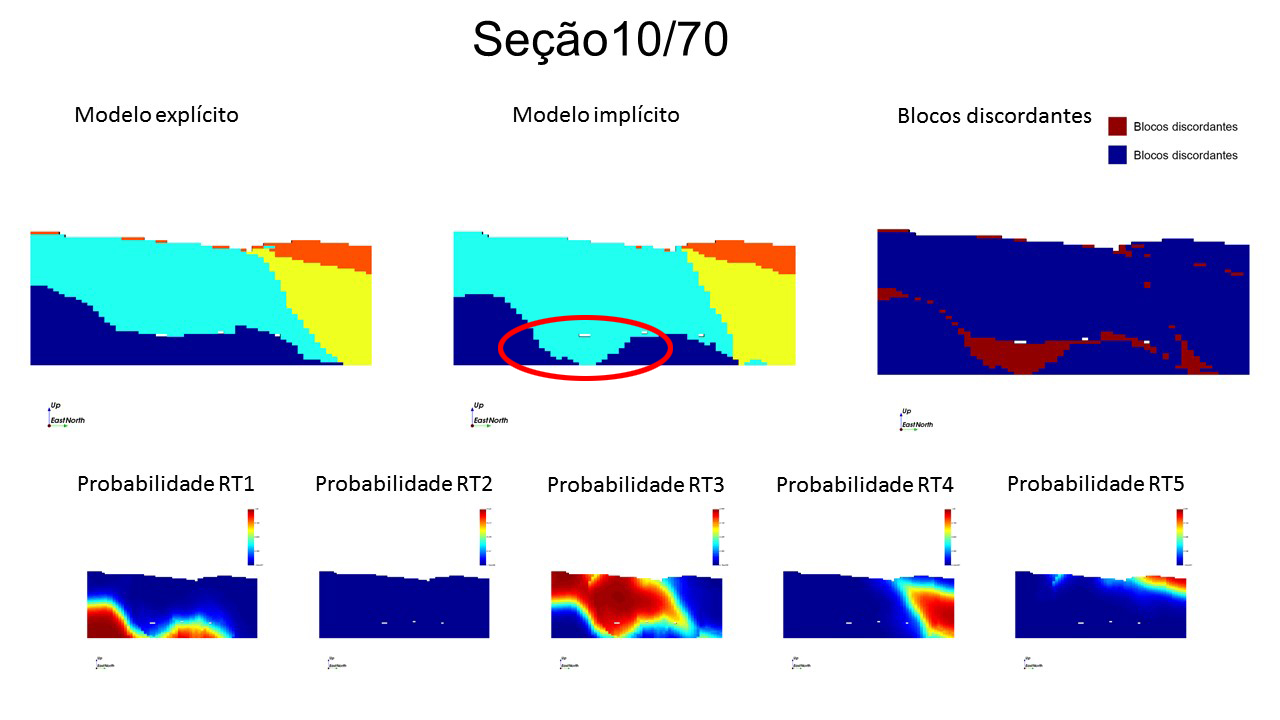
\includegraphics[width=0.9\textwidth]{estudo_de_caso/secaox10}
	\end{center}
	%\legend{Fonte: Modificado de \citeonline{maureira}}
\end{figure}

Na seção da \autoref{secaox37}, a região destacada pela elipse vermelha mostra uma estrutura desenhada pelo geomodelador no modelo explícito, com formas suaves e intricadas, de difícil reprodução pelos métodos matemáticos, a não ser em casos de alta densidade amostral. 

\begin{figure}[H]
	\caption{\label{secaox37}Seção vertical 37/70 em x.}
	\begin{center}
		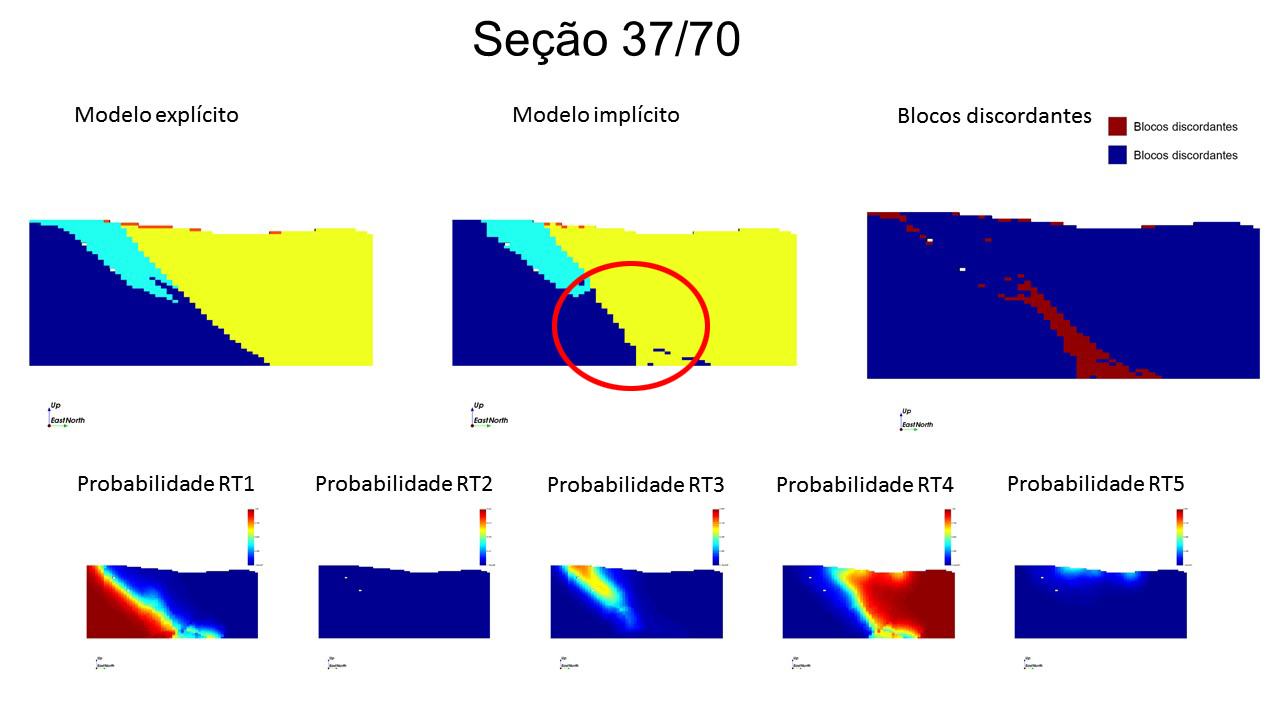
\includegraphics[width=0.9\textwidth]{estudo_de_caso/secaox37}
	\end{center}
	%\legend{Fonte: Modificado de \citeonline{maureira}}
\end{figure}

As estruturas presentes na seção 56 (\autoref{secaox56}), são estruturas pouco complexas, e foram bem reproduzidas pelo algoritmo.

\begin{figure}[H]
	\caption{\label{secaox56}Seção vertical 56/70 em x.}
	\begin{center}
		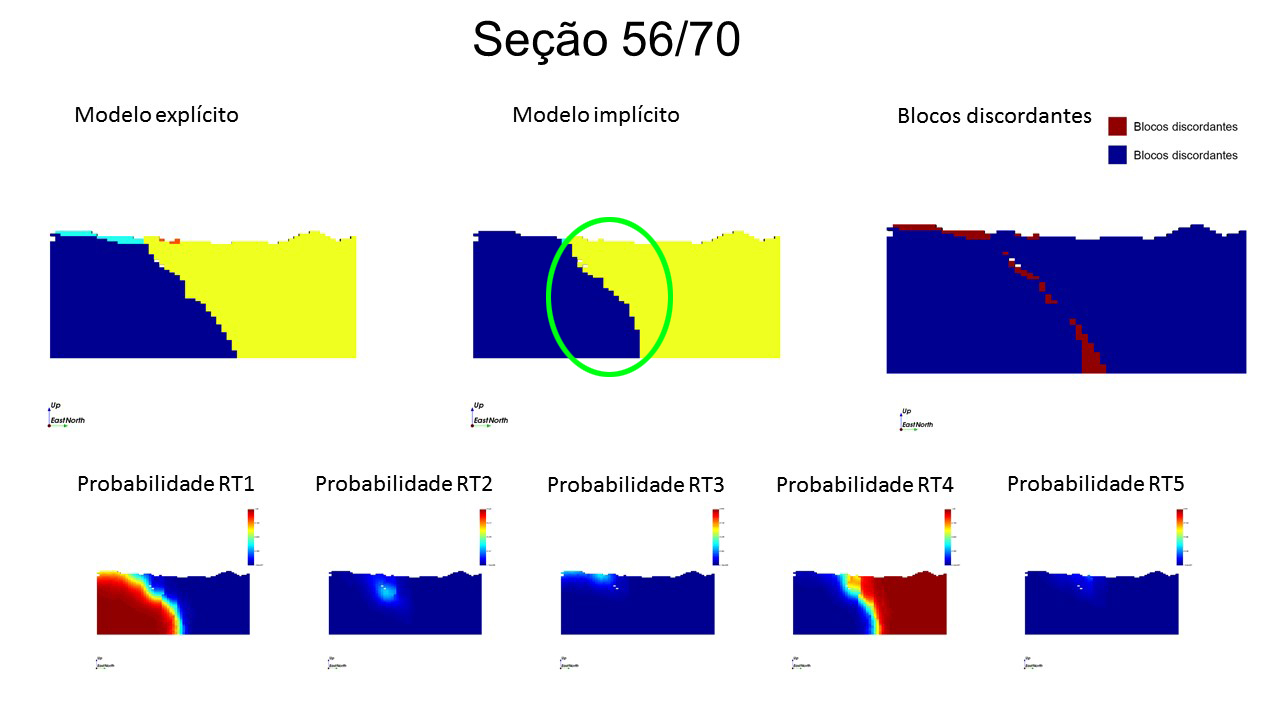
\includegraphics[width=0.9\textwidth]{estudo_de_caso/secaox56}
	\end{center}
	%\legend{Fonte: Modificado de \citeonline{maureira}}
\end{figure}

A seção da \autoref{secaox67}, mostra destacado pela elipse vermelha, uma estrutura que não foi bem reproduzida, o algoritmo deu mais volume à litogia 1 e menos à litologia 2 em relação ao modelo criado explicitamente. 

\begin{figure}[H]
	\caption{\label{secaox67}Seção vertical 67/70 em x.}
	\begin{center}
		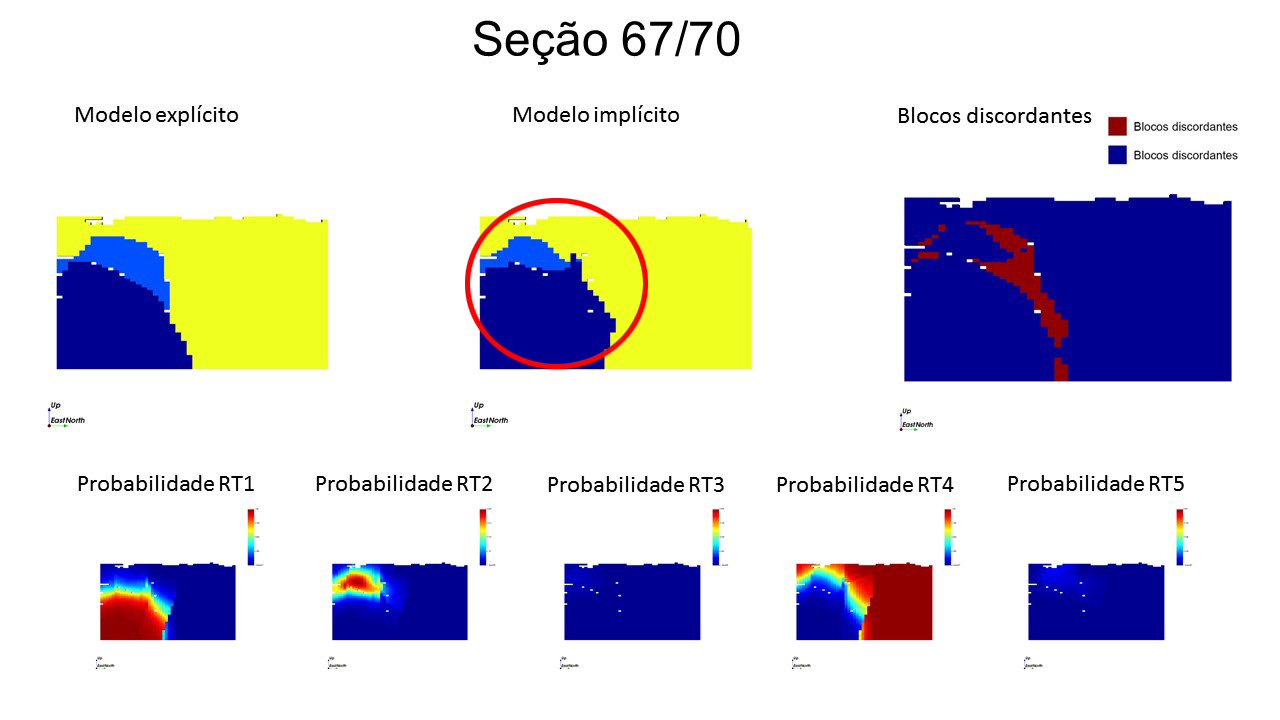
\includegraphics[width=0.9\textwidth]{estudo_de_caso/secaox67}
	\end{center}
	%\legend{Fonte: Modificado de \citeonline{maureira}}
\end{figure}

Na direção y, o modelo apresenta 60 seções. A seção 16 (\autoref{secaoy16}) exibe poucos blocos discordantes, o algoritmo reproduziu satisfatoriamente as estruturas interpretadas pelo geomodelador.

\begin{figure}[H]
	\caption{\label{secaoy16}Seção vertical 16/60 em y.}
	\begin{center}
		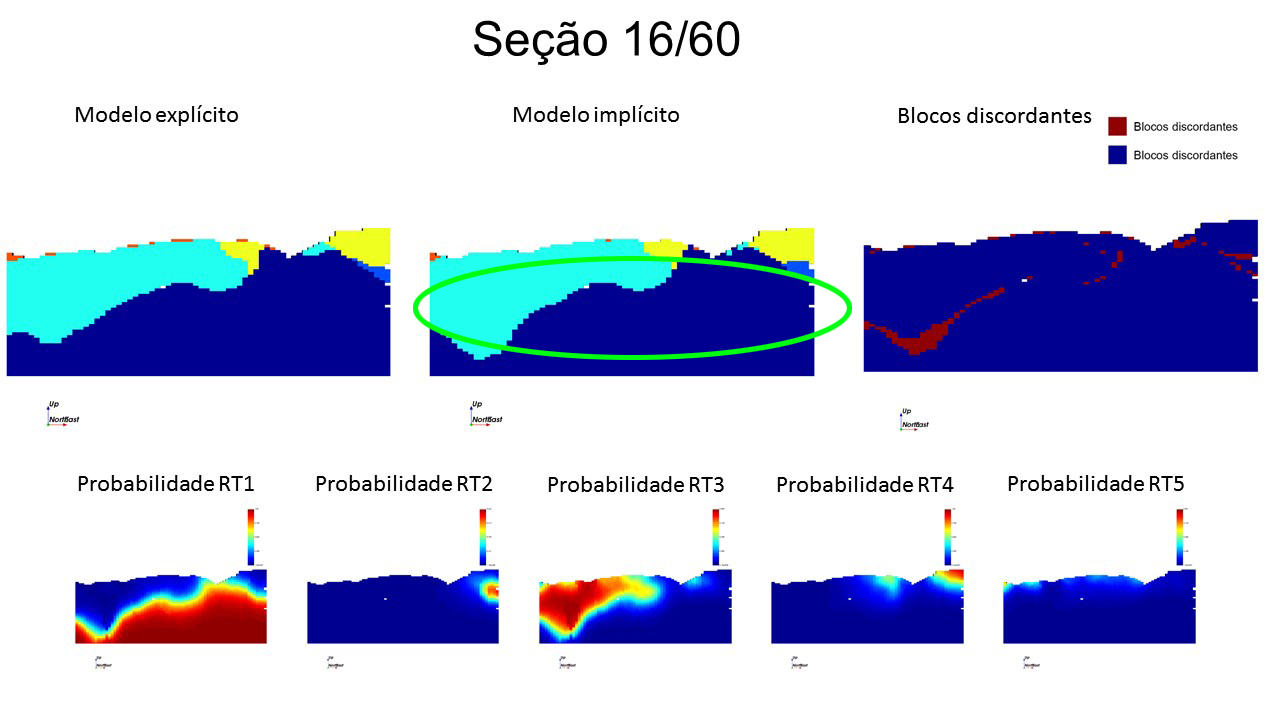
\includegraphics[width=0.9\textwidth]{estudo_de_caso/secaoy16}
	\end{center}
	%\legend{Fonte: Modificado de \citeonline{maureira}}
\end{figure}

Embora as estruturas interpretadas exibidas na \autoref{secaoy27} sejam bastante complexas, o algoritmo as reproduziu de forma razoável. 

\begin{figure}[H]
	\caption{\label{secaoy27}Seção vertical 27/60 em y.}
	\begin{center}
		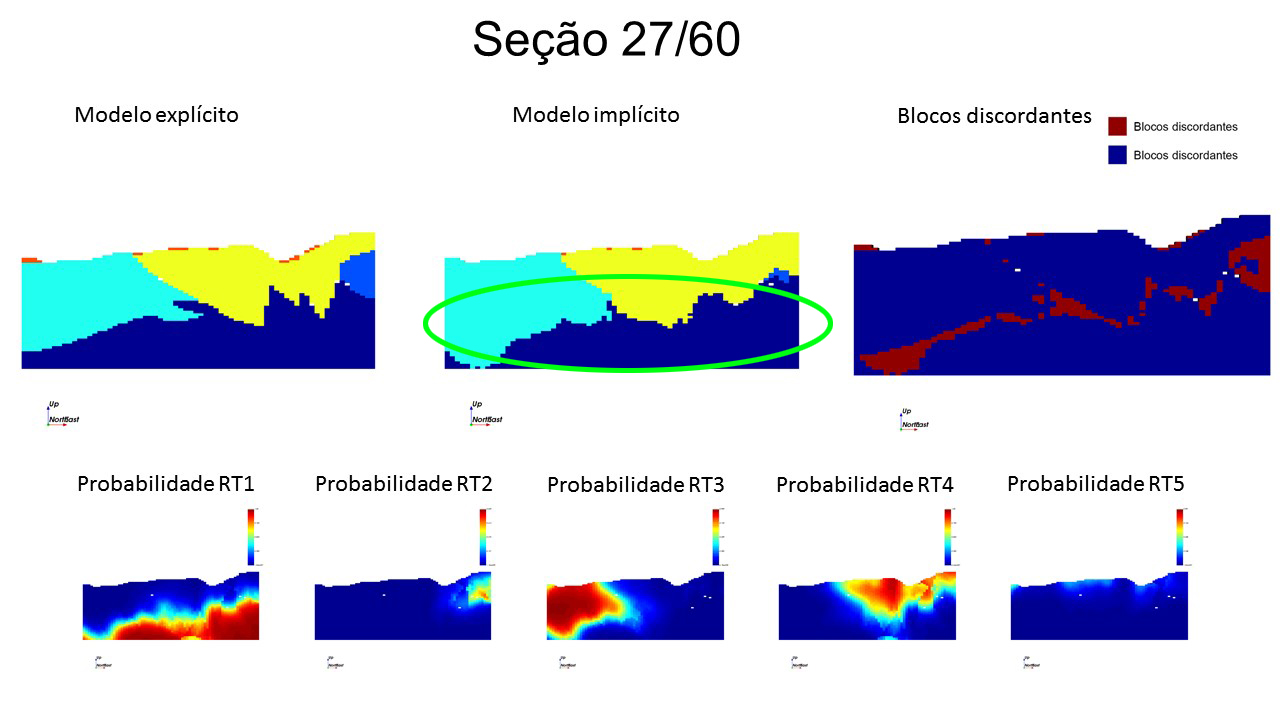
\includegraphics[width=0.9\textwidth]{estudo_de_caso/secaoy27}
	\end{center}
	%\legend{Fonte: Modificado de \citeonline{maureira}}
\end{figure}

Novamente, o método implícito reproduziu de forma satisfatória as estruturas interpretadas na \autoref{secaoy43}. 

\begin{figure}[H]
	\caption{\label{secaoy43}Seção vertical 43/60 em y.}
	\begin{center}
		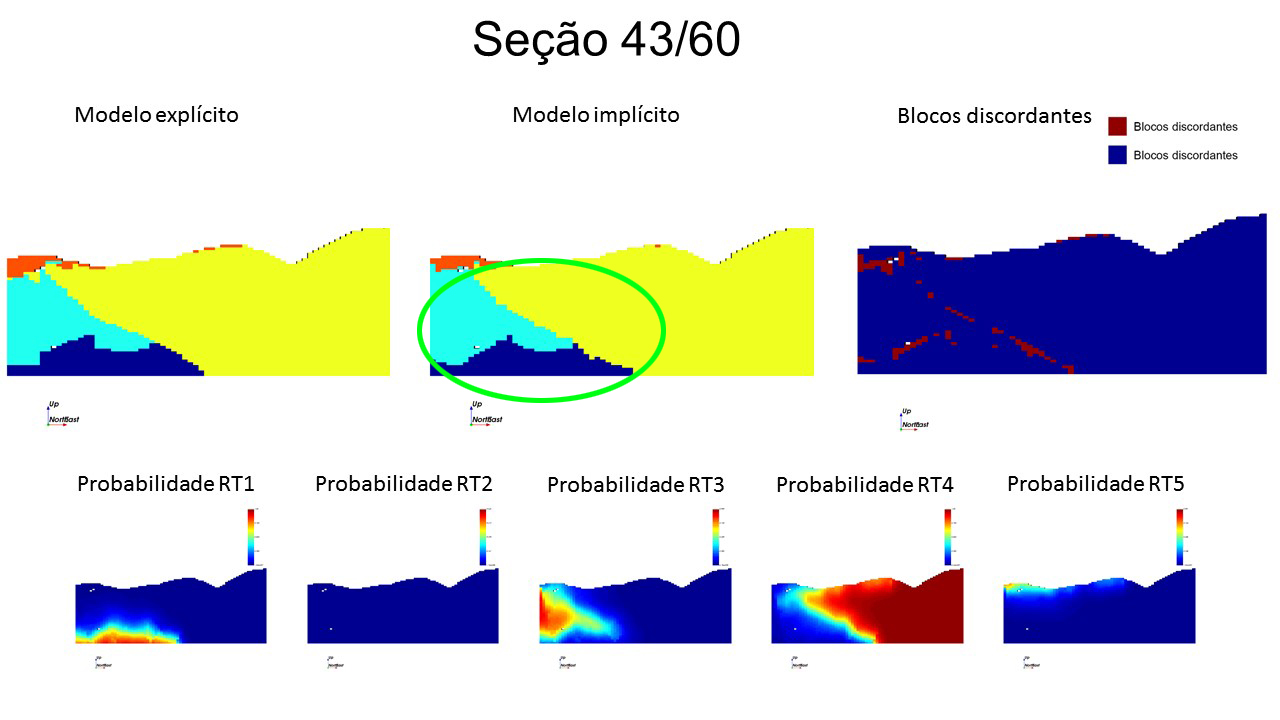
\includegraphics[width=0.9\textwidth]{estudo_de_caso/secaoy43}
	\end{center}
	%\legend{Fonte: Modificado de \citeonline{maureira}}
\end{figure}

A seção da \autoref{secaoy54} mostra, na zona destacada em vermelho, blocos atribuídos com a litologia 1 pelo geomodelador enquanto no modelo implícito esses blocos são atribuídos com a litologia 3. Novamente, essa é uma região sem amostras de litologia 1, o geomodelador, provavelmente, contou com sua experiência ou informação adicional para inferir a litologia desses blocos.

\begin{figure}[H]
	\caption{\label{secaoy54}Seção vertical 54/60 em y.}
	\begin{center}
		\includegraphics[width=0.9\textwidth]{estudo_de_caso/secaoy54}
	\end{center}
	%\legend{Fonte: Modificado de \citeonline{maureira}}
\end{figure}

Nesse estudo de caso, a aplicação do \textit{servo system} torna o modelo mais discordante em relação ao modelo de referência fornecido para comparação. Embora, as proporções dos dados ou dados desagrupados possam ser reproduzidas.

\section{Discussão}

A informação geológica é incorporada ao modelo através, não só do cálculo das distâncias assinaladas anisotrópicas, como também pelas direções de continuidade e efeito pepita dos variogramas. Limites suaves entre as litologias são garantidos pelo emprego da krigagem ordinária. Embora a complexidade geológica de pequena escala não seja bem reproduzida, devido ao efeito de suavização da krigagem, as grandes estruturas são bem representadas pelo algoritmo. A aplicação de um elipsoide de busca grande o suficiente e dados condicionantes em grandes quantidades aproximam os resultados da krigagem ordinária à krigagem global, evitando o surgimento de artefatos nos modelados gerados. O método implementado para múltiplos domínios geológicos evita sobreposição de litologias ou a necessidade de estabelecer qualquer tipo de ordem de prioridade para sua modelagem.

À primeira vista a modelagem dos variogramas para todas as categorias parece uma tarefa laboriosa e tediosa. Todavia, O comportamento contínuo das distâncias assinaladas os torna fáceis de modelar, e em muitos casos são semelhantes entre si, permitindo o uso de um mesmo modelo para todas as litologias. 

Algoritmos de modelagem geológica implícita devem satisfazer seis critérios estabelecidos por \citeonline{mclennan}: simplicidade, velocidade, objetividade, integração de dados, avaliação de incertezas e realismo geológico. O método proposto foi avaliado à luz desses critérios, a partir de observações feitas ao longo desse trabalho e do trabalho de \citeonline{maureira}. Pontos positivos e negativos são aqui apresentados.

\begin{itemize}
\item Simplicidade: O algoritmo é de simples implementação e não envolve nenhuma equação matemática complicada. A ideia de uma distância assinalada para cada domínio é de fácil compreensão;
\item Velocidade: O algoritmo é baseado em krigagem, que são métodos notadamente rápidos. A limitação é quanto ao número máximo de dados condicionantes usados na vizinhança de busca ao estimar cada bloco (acima de 200 tornam a execução bastante demorada);
\item Objetividade: A abordagem implícita surgiu para eliminar a subjetividade dos métodos explícitos de modelagem. É esperado que modelos sejam reproduzidos com exatidão quando os parâmetros envolvidos nos cálculos sejam os mesmos. Os modelos não estão sujeitos à influência individual de cada geomodelador;
\item Integração de dados: O algoritmo é flexível quanto à incorporação de novos dados do mesmo tipo. Entretanto, informação secundária (de outro tipo) não pode ser adicionada;
\item Avaliação de incerteza: O algoritmo não avalia incerteza baseado em múltiplas realizações equiprováveis de modelos geológicos. Contudo, uma forma alternativa de medição heurística da incerteza, baseada na transformação das distâncias estimadas em probabilidades, é implementada no método.
\item Realismo geológico: Modelos são considerados realísticos quando possuem concordância com a interpretação, e evidencias geológicas coletadas pelo geomodelador \cite{maureira}. A comparação da \autoref{comparacao}, mostra que o algoritmo reproduz satisfatoriamente, dadas suas limitações, as estruturas interpretadas. A krigagem ordinária, base do algoritmo, possui efeito de suavização. Então, embora estruturas de larga escala sejam bem reproduzidas, a reprodução da complexidade geológica de pequena escala fica comprometida.
\end{itemize}

Um geomodelador experiente dificilmente será substituído por um código e um computador. Porém, o algoritmo proposto é de grande ajuda, como método complementar à modelagem explícita. Principalmente, em fases iniciais do projeto ou na criação de proto modelos que devem ser refinados, poupando tempo e trabalho. À medida que a densidade amostral aumenta, o modelo implícito se torna mais próximo do modelo explícito.

Por fim, as vantagens e desvantagens da metodologia apresentada são discutidas.

Vantagens:

\begin{itemize}
\item Os modelos podem ser atualizados com facilidade e rapidez conforme novos dados são obtidos. Não há necessidade de nova digitalização manual;
\item Usando os mesmos parâmetros, os modelos são reproduzidos com exatidão, tornando a checagem e auditoria externa simples;
\item Uma variedade de análises de sensibilidade pode ser aplicadas ao modelo, variando parâmetros envolvidos na interpolação e nos variogramas das distâncias assinaladas;
\item O processo é rápido, poupando tempo e trabalho de geomodeladores na tediosa tarefa de construir e digitalizar manualmente seções verticais e horizontais.
\end{itemize}

Desvantagens:

\begin{itemize}
\item A interpolação das distâncias assinaladas pode impedir que um profissional treinado interprete estruturas e tendências da geologia que possam levar a melhores resultados;
\item O algoritmo é baseado em krigagem, então, apenas relações lineares entre domínios são modeladas (caso não existam amostras suficientes). A modelagem de estruturas complexas e curvilíneas depende de outros métodos geoestatísticos. Além disso, a propriedade suavizadora da krigagem compromete a modelagem da geologia de pequena escala;
\item O comportamento não estacionário das distâncias assinaladas torna a inferência do alcance dos variogramas arbitrária e questionável;
\item Não avalia incerteza baseado em múltiplas realizações equiprováveis do modelo;
\item O efeito de borda pode criar estruturas irreais nos limites do modelo.
\end{itemize}

\chapter{Considerações finais}

Essa dissertação propôs como meta investigar a aplicabilidade da modelagem geológica implícita com funções distância assinaladas como método substituto ou auxiliar aos métodos clássicos de modelagem. Para tanto, foram apresentados dois objetivos específicos:

\begin{enumerate}
\item Operacionalizar o método no software geoestatístico de código aberto \textit{SGeMS},
desenvolvendo um \textit{plug-in} funcional em \textit{python}.
\item Conduzir um estudo de caso em um banco de dados real e verificar a qualidade do
modelo gerado pela metodologia proposta, comparando-o a um modelo de referência.
\end{enumerate}

Quanto ao primeiro objetivo, um \textit{plug-in} foi desenvolvido e validado. É intuitivo e de fácil utilização. Uma alternativa mais amigável ao usuário em relação à rotina do \textit{GSLib} desenvolvida por \citeonline{maureira}.

A partir do estudo de caso (\autoref{estudo_de_caso}) foi possível concluir que a modelagem geológica implícita com funções distância assinaladas é um método simples, rápido e de grande auxílio ao geomodelador. Apesar de não substituir completamente os métodos explícitos, o método gerou um modelo geológico bastante semelhante ao modelo criado explicitamente, tomado como referência, em poucos minutos e que pode ser facilmente replicado, permitindo simples checagem e auditoria externa. Ainda é possível avaliar, mesmo que de uma forma heurística, a incerteza associada ao modelo geológico e reproduzir proporções, evitando a introdução de viés.

A modelagem geológica é uma etapa fundamental da avaliação depósitos minerais já que as estimativas e simulações dependem de domínios estacionários. Além disso, um bom modelo geológico pode trazer maior rentabilidade ao empreendimento, ou até mesmo ser crucial para a decisão de investir ou não baseada nos resultados do relatório de viabilidade, uma vez que a maior causa de fracasso nos empreendimentos mineiros é a falta de conhecimento a respeito do corpo mineralizado.

\section{Recomendações para trabalhos futuros}

Como recomendação para trabalhos futuros:

\begin{itemize}
\item Repetir o estudo de caso em banco de dados com menor densidade amostral e em depósitos que apresentem geologia mais complexa;
\item Aprimorar o \textit{plug-in} desenvolvido, se possível, reescrevendo-o em \textit{C++}. Em especial o algoritmo do \textit{servo system}, que pode se tornar muito demorado em banco de dados volumosos. 
\item Investigar outras formas, além da \textit{softmax transformation}, para medir incertezas nos contatos geológicos. \citeonline{mclennan2006implicit} propuseram uma metodologia para quantificar incertezas através da técnica de \textit{bootsrap}, enquanto \citeonline{munroe2012methodology,wildedeutschcalibrate} propuseram calibrar uma banda de incertezas ao longo dos contatos entre os domínios;
\item Investigar a viabilidade de simular as distâncias assinaladas, avaliando assim, a incerteza baseada em múltiplas realizações equiprováveis do modelo geológico;
\item Estudar a possibilidade de agregar ao método informação secundária, usada pelo geomodelador para construir modelos explícitos;
\item Implementar o \textit{plug-in} independentemente de um \textit{grid} de interpolação, permitindo a criação de modelos (\textit{wireframes}) em qualquer resolução;
\item Desenvolver técnicas híbridas de modelagem geológica, considerando as abordagens explícita, implícita e estocástica.
\end{itemize}

% ----------------------------------------------------------
% ELEMENTOS PÓS-TEXTUAIS
% ----------------------------------------------------------
\postextual
% ----------------------------------------------------------

% ----------------------------------------------------------
% Referências bibliográficas
% ----------------------------------------------------------
\bibliography{Ref_bibliografica_dissertacao}

% ----------------------------------------------------------
% Glossário
% ----------------------------------------------------------
%
% Consulte o manual da classe abntex2 para orientações sobre o glossário.
%
%\glossary

% ----------------------------------------------------------
% Apêndices
% ----------------------------------------------------------

% ---
% Inicia os apêndices
% ---
\begin{apendicesenv}

% Imprime uma página indicando o início dos apêndices
\partapendices

% ----------------------------------------------------------
\chapter{Algoritmo em python que calcula as distâncias anisotrópicas assinaladas (\textit{signed distances})}\label{apendicea}
% ----------------------------------------------------------

\includepdf[pages=-]{apendices/signed_distances}

% ----------------------------------------------------------
\chapter{Algoritmo em python que interpola as distancias assinaladas e cria o modelo geológico (\textit{interpolator})}\label{apendiceb}
% ----------------------------------------------------------

\includepdf[pages=-]{apendices/interpolator}

\end{apendicesenv}
% ---


% ----------------------------------------------------------
% Anexos
% ----------------------------------------------------------

% ---
% Inicia os anexos
% ---
\begin{anexosenv}
%
% Imprime uma página indicando o início dos anexos
\partanexos
%
% ---
\chapter{Arquivo de parâmetro usado na validação}\label{anexo}
% ---
\verbatiminput{anexos/dfmod_par_dessert.txt}
%
% ---
%\chapter{Cras non urna sed feugiat cum sociis natoque penatibus et magnis dis
%parturient montes nascetur ridiculus mus}
% ---
%
%\lipsum[31]
%
% ---
%\chapter{Fusce facilisis lacinia dui}
% ---
%
%\lipsum[32]
%
\end{anexosenv}

%---------------------------------------------------------------------
% INDICE REMISSIVO
%---------------------------------------------------------------------
%\phantompart
%\printindex
%---------------------------------------------------------------------

\end{document}
